% !TEX encoding = UTF-8 Unicode
\documentclass[
  12pt,                        % フォントサイズ
  openany,                     % 省の始まりを奇数ページに限定しない
%  draft,                       % 下書き用 画像を読み込まないのでタイプセットが早く済む
]{jsbook}

%====================================================================================================
%===== use package
\usepackage[dvipdfmx]{graphicx}% figure環境:\begin{figure}
\usepackage[top=20mm, bottom=25mm, left=20mm, right=20mm]{geometry}
                               % 余白の設定
\usepackage{amsmath,amssymb}   % 数式環境:\begin{align}
% \usepackage{bm}                % 太字かつイタリックでベクトルを表現:\bm{} 
% \usepackage{lscape}            % 本文を横向きに配置:\begin{landscape}
% \usepackage{ascmac}            % 罫線付きテキスト:\begin{screen}, \begin{itembox}, ...
% \usepackage{fancybox}          % 罫線付きテキスト:\doublebox{}, \ovalbox{}, ...
\usepackage{fancyhdr}          % fancy header環境
% \usepackage{mediabb}           % \includegraphycsでpdfを読み込む, pngとかが読めなくなる副作用あり
% \usepackage{longtable}         % 頁をまたぐ表の作成
% \usepackage{multirow}          % 表のセルを縦に結合
\usepackage[dvipdfmx,          % PDF環境
 bookmarks        =true,       % 目次の作成するか
 bookmarksnumbered=false,      % 節を目次に載せるか
 bookmarkstype    =toc,        % tocはデフォルト
 bookmarksopen    =true,       % ツリー状の目次
 hidelinks,                    % リンクに色や枠をつけない
 colorlinks       =false,      % リンクをカラー表記にするか
 linkbordercolor  ={1 1 0},    % リンクを囲む罫線の色
 citebordercolor  ={0 1 1},    % 参考文献のリンクの色
 urlbordercolor   ={1 0 1},    % URLのリンクの色
 pdfstartview     ={FitH -32768},
                               % PDFを開いた時のビューの初期値
 pdftitle         ={修士論文},
                               % PDF Title
 pdfsubject       ={九州大学大学院 理学府 物理学専攻 粒子物理学分野 素粒子実験研究室 xxxx年度 修士論文},
                               % PDF Subject
 pdfauthor        ={},% PDF Author
 pdfkeywords      ={}          % PDF Keywords
 pdfborder        ={1 1 1},    % PDFのリンクの幅
]{hyperref}                    % ハイパーリンクの使用
\usepackage{pxjahyper}         % pdfで日本語目次を使用
\usepackage{url}               % URL環境:\url{}
\usepackage{dcolumn}           % 表中の任意の位置で揃える D{.}{.}{-1}
\usepackage{mathcomp}          % °=\tcdegree, ℃ = \tccelsius
\usepackage{subcaption}        % 図1.1(a), (b)のように図を並べられる。
% \usepackage{color}             % 文字に色を付けるためのパッケージ
% \usepackage{mathtools}         % \begin{matrix*}[l]で行列要素を左寄せが可能

%===================================================================================================
%===== set length
\setlength { \textheight } { 37 \baselineskip }
\setlength { \textwidth } { \fullwidth }
\setcounter{tocdepth}{3}

%====================================================================================================
%===== set header
\pagestyle{fancy} 
\fancyhead{}
\fancyhead[LO,LE]{\leftmark}
\fancyhead[RO,RE]{\rightmark}
\cfoot{\thepage}

%====================================================================================================
%===== new parameter, new command
\newif\ifabstract
%\newcounter{footnotecounter}
%\setcounter{footnotecounter}{1}

\makeatletter
\def\fiscalyear#1{\def\@fiscalyear{#1}} % 年度
\def\supervisor#1{\def\@supervisor{#1}} % 指導教員
\def\university#1{\def\@university{#1}} % 大学
\def\department#1{\def\@department{#1}} % 所属学部/学府
\def\labolatory#1{\def\@laboratory{#1}} % 所属研究室

\newcommand{\maketitlepage}{% 回覧版/製本版のタイトル
 \begin{titlepage}
  \begin{center}
   {\Large \@fiscalyear{}年度 修士論文}   \\ 
   \vspace*{125pt}
   {\Large \@title{}}                     \\[11pt]
   {\large \@university{} \@department{}} \\
   {\large \@laboratory{}}                \\[15pt]
   \vspace{40pt}
   {\large \@author{}}                    \\[1ex]
   {\large 指導教員\ \@supervisor{}}      \\[1em]
   \@date{}                               \\
   \vspace{100pt}
   
\includegraphics[width=3cm]{./Figure/Introduction/KyushuUniversityLogo.eps}
  \end{center}
 \end{titlepage}
}
\renewcommand{\maketitle}{% 修論概要提出時のタイトル
 \thispagestyle{empty}
 \begin{center}
  {\Large \@title{}}            \\
  \@university{} \@department{} \\
  \@laboratory{}                \\
  \@author{}                    \\[1ex]
  指導教員\ \@supervisor{}      \\
  \mbox{}                       \\
 \end{center}
}
\makeatother

% ベクトル演算子の定義
% \newcommand{\divergence}{\mathrm{div}\,}
% \newcommand{\grad}{\mathrm{grad}\,}
% \newcommand{\rot}{\mathrm{rot}\,}

% 空白ページの挿入
\newcommand{\blackpage}{\newpage\thispagestyle{empty}\mbox{}\newpage}

% 目次の生成
\newcommand{\makeindexpage}{
 \tableofcontents
 \listoffigures
 \listoftables
}

% ヘッダに表示する項目
\renewcommand{\headfont}{\bfseries}
\renewcommand{\chaptermark}[1]{\markboth{第\ \thechapter\ 章~#1}{}}
\renewcommand{\sectionmark}[1]{\markright{\thesection \ \ #1}{}}

%====================================================================================================
%===== タイトルのパラメータ
\fiscalyear{2022}
\title     {電子陽電子ヒッグスファクトリーのための\\ジェット測定技術の研究}
\author    {尾上\ 友紀}
\supervisor{末原\ 大幹\ 川越\ 清以}
\university{九州大学大学院}
\department{理学府 物理学専攻}
\labolatory{粒子物理学分野 素粒子実験研究室}
\date      {\today}

%====================================================================================================
%===== 概要提出時は「\abstracttrue」
%===== 回覧版/製本版は「\abstractfalse」
\abstractfalse

%====================================================================================================
%===== begin document
\begin{document}
\pagestyle{headings}

%----------------------------------------------------------------------------------------------------
%----- タイトル
\ifabstract\else
 \maketitlepage
 \blackpage
\fi

%----------------------------------------------------------------------------------------------------
%----- 概要
% !TEX root = ../MasterThesis_Onoe.tex
% 上記はただのコメントではなく親ファイルの場所を教えているので
% 消してしまうとファイルごとのタイプセットができなくなるので注意。
% 親ファイル名を変更したときはここも変更する。

\begin{center}
%概要集に出すときにはタイトルや氏名が必要なので\iffalseを \ifture にする。
%本文で使用する場合は不要なので \iffalse にする。
\iffalse
\thispagestyle{empty}
{\Large 修士論文テンプレート}\\
九州大学大学院 理学府 物理学専攻 \\ 粒子物理学分野 素粒子実験研究室 \\
素粒子\ 実験 \\[1ex] 指導教員\ 氏\ 名\\   \\
\fi
{\huge 概要}\\
\end{center}

本研究では、電子陽電子ヒッグスファクトリーにおいて衝突により発生するジェット測定技術の研究として、2つの研究を行った。国際リニアコライダー(International Linear Collider:ILC)計画は次世代電子陽電子衝突型加速器であり、その検出器案であるシリコンタングステン電磁カロリメータ Sillicon Tangsten Electromagnetic Calorimeter (SiW-ECAL) の性能評価に関する研究を行った。
ILC は現在建設が検討されている全長約 20 kmの線形加速器で、電子と陽電子の衝突によって生じるジェットの解析により Higgs 粒子の精密測定やダークマターの候補となる新粒子の探索などが可能とされ、標準理論を超える物理を切り拓く足がかりとして期待されている。ILC で重要となるイベントにはジェットが含まれ、ILC の目標感度を達成するためにはおおよそ

\cite{sample}

%----------------------------------------------------------------------------------------------------
%----- 目次
\ifabstract\else
 \blackpage
 \makeindexpage
\fi

%----------------------------------------------------------------------------------------------------
%----- 本章
\ifabstract\else
 % !TEX root = ../MasterThesis_Onoe.tex
% 上記はただのコメントではなく親ファイルの場所を教えているので
% 消してしまうとファイルごとのタイプセットができなくなるので注意。
% 親ファイル名を変更したときはここも変更する。

\chapter{序論} \label{sec:Intruduction}
 本章では、はじめに1.1節で素粒子とそれらに働く相互作用を説明する標準模型(The Standard Model, SM)について述べる。そして1.2節にて将来の電子陽電子ヒッグスファクトリーである、国際リニアコライダー計画(International Linear Collider, ILC)の概要に触れたのち、1.3節でILCが探索する物理、1.4節でILCのについて述べる。
\section{素粒子標準理論}
 素粒子とは、物質を構成している究極要素をさす名称である。そして素粒子物理学は、それら構成要素とその間に働く相互作用の性質を解明する学問である。現代の素粒子物理学では、すべての現象を説明するための基本的な枠組みとして図\ref{sm}のような標準模型を掲げており、これは現時点の実験データと高い精度で一致することが確認されている。\\

\begin{figure}[htbp]
	\begin{center}
 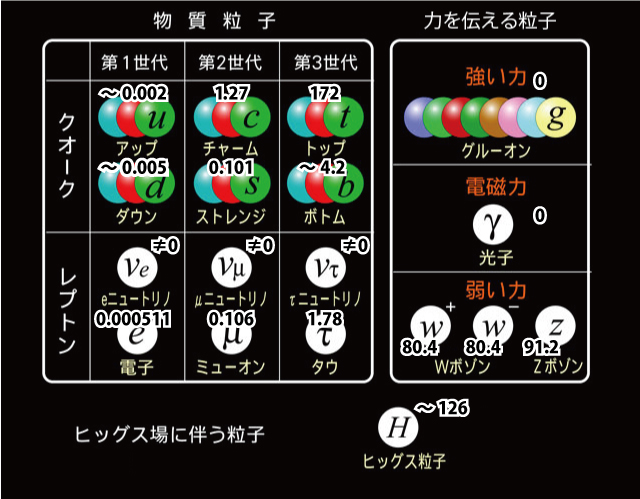
\includegraphics[keepaspectratio, scale=0.4]
 	{Figure/Introduction/sm.jpg}
 		\caption{素粒子の標準模型}
 		\label{sm}
	\end{center}
\end{figure}

 標準理論は、主に次に挙げる2つの公理に沿って記述されている。1つ目に、物質の究極要素である素粒子はクォークとレプトンというスピン1/2のフェルミオンである。2つ目に、素粒子の相互作用はゲージ粒子によって記述され、標準理論における相互作用は電磁相互作用・弱い相互作用・強い相互作用の3つである。\\
 物質の化学的性質を失わない最小単位は分子であり、分子はさらに原子の組み合わせによって構成されている。そして原子は原子核と電子によって構成されており、原子核は陽子と中性子のような核子からなっている。この核子を構成するものがクォークであり、標準模型においては6種類存在する。また同様に素粒子であり、核力のような強い相互作用をしないものをレプトンと呼び、同様に6種類存在する。クォーク・レプトンともに3つの世代と2つの電荷タイプをもっており、世代の高い粒子ほど重いため弱い相互作用により低い世代のクォークへと崩壊する。\\
 素粒子の相互作用を媒介するスピン1のゲージ粒子には、フォトン・Wボソン、Zボソン、グルーオンの4種類がある。このうち電磁相互作用と弱い相互作用は統一され電弱相互作用と呼ばれており、

標準模型は物質を構成する粒子であるフェルミオンと力を媒介する粒子であるボソンから構成される。またフェルミオンは、陽子や中性子を構成する6種類のクォークと電子やニュートリノなどのレプトンに大きく分けられる。クォーク、レプトンはそれぞれ電荷によって2つに分けられ、さらに世代によって3つに分けられる。

\section{国際リニアコライダー計画: ILC}

\section{ILCの物理}

\subsection{新物理探索}

\section{ILCにおける検出器}

\subsection{Particle Flow Algorithm: PFA}

\subsection{International Large Detector: ILD}

\subsubsection{飛跡検出器}

\subsubsection{電磁カロリメータ}

\subsubsection{ハドロンカロリメータ}

\subsubsection{ミューオン検出器}

\section{ILCにおける物理解析}

\subsection{事象再構成}

\section{本研究の目的}
 % !TEX root = ../MasterThesis_Onoe.tex
% 上記はただのコメントではなく親ファイルの場所を教えているので
% 消してしまうとファイルごとのタイプセットができなくなるので注意。
% 親ファイル名を変更したときはここも変更する。

\chapter{シリコンタングステン電磁カロリメータ} \label{sec:1.Siwecal}
本章では、ILDのシリコンタングステン電磁カロリメータについて説明する。まず検出器を理解する上で必要な粒子と物質の相互作用について述べたのち、カロリメータの検出原理やシリコン検出器の検出原理について述べる。そして現在のILDにおけるシリコンタングステン電磁カロリメータの読み出し方法、またASICの設計性能やの読み出し方法、現在の技術プロトタイプについて説明する。
\section{入射粒子と物質の相互作用}
素粒子実験で捉えたい素粒子やハドロンは、粒子と物質との相互作用によって捉えることができる。よって本節では入射粒子の種類ごとに物質との相互作用について述べる。
\subsection{荷電粒子}
荷電粒子のエネルギー損失の要因には、主に電離損失と制動放射が挙げられ、特にエネルギーの低いところでは電離損失の割合が、エネルギーの高いところでは制動放射の割合が高くなる。以下ではそれぞれについて述べる。
\subsubsection{電離損失}
荷電粒子は物質を通過することで、物質中の原子を電離あるいは励起させ電離エネルギー損失を生じる。この電離エネルギー損失は原子中の電子によるクーロン散乱によるものが支配的であり、Bethe-Blochの式に従う。
\begin{equation}
-\frac{dE}{dx} = 4\pi N_A {r_e}^2 m_e c^2 z^2 \frac{Z}{A} \frac{1}{{\beta}^2} \left[ \frac{1}{2} \ln(\frac{2m_e c^2{\beta}^2{\gamma}^2W_{max}}{I^2}) -{\beta}^2 - \frac{\delta(\beta \gamma)}{2} \right]
\end{equation}

\begin{table}[H]
 \label{table:bethe}
 \centering
  \begin{tabular}{clll}
   \hline \hline
   &変数 & 値または単位 \\
   \hline
&$N_A $: アボガドロ定数 & $6.022 \times 10^23 {\si{\mol}}^{-1}$\\
&$r_e$ : 古典電子半径&2.817 fm\\ 
&$m_e$ : 荷電粒子の質量 &0.511MeV\\
&$c$ : 光速 & $2.998 \times 10^8 m/s$\\
&$z$ : 入射粒子の電荷& - \\
&$Z$ : 物質の原子番号 & - \\
&$A$ : 物質の相対原子質量 & g\ ${\si{\mol}}^{-1}$ \\
&$\beta$ : 入射粒子の$v/c$ & - \\
&$\gamma$ : $1\sqrt{1-{\beta}^2}$ & - \\
&$W_{max}$ : 1回の衝突で物質に与える最大エネルギー & MeV\\
&$I$ : 物質の平均イオン化ポテンシャル &eV\\
&$\delta(\beta \gamma)$ : 密度効果による電離エネルギー損失の補正 & $\sqrt{\rho \langle Z/A\rangle } \times 28.816eV$\\
  \end{tabular}
\end{table}
Bethe-Blochの式より、電離エネルギー損失$-dE/dx$は荷電粒子の入射速度に依存する。様々な物質に対する電離エネルギー損失と入射速度の関係を図\ref{dE/dx}に示す。入射速度の小さいとき電離エネルギー損失は$1/{\beta}^2$に比例しており、$\beta \gamma  \approx 3 \sim 4$で電離エネルギー損失は最小値に達する。これを最小電離損失といい、この領域にある粒子をMIP(Minimum Ionization Particle)と呼ぶ。
 \begin{figure}[h]
 \label{dE/dx}
\begin{center}
 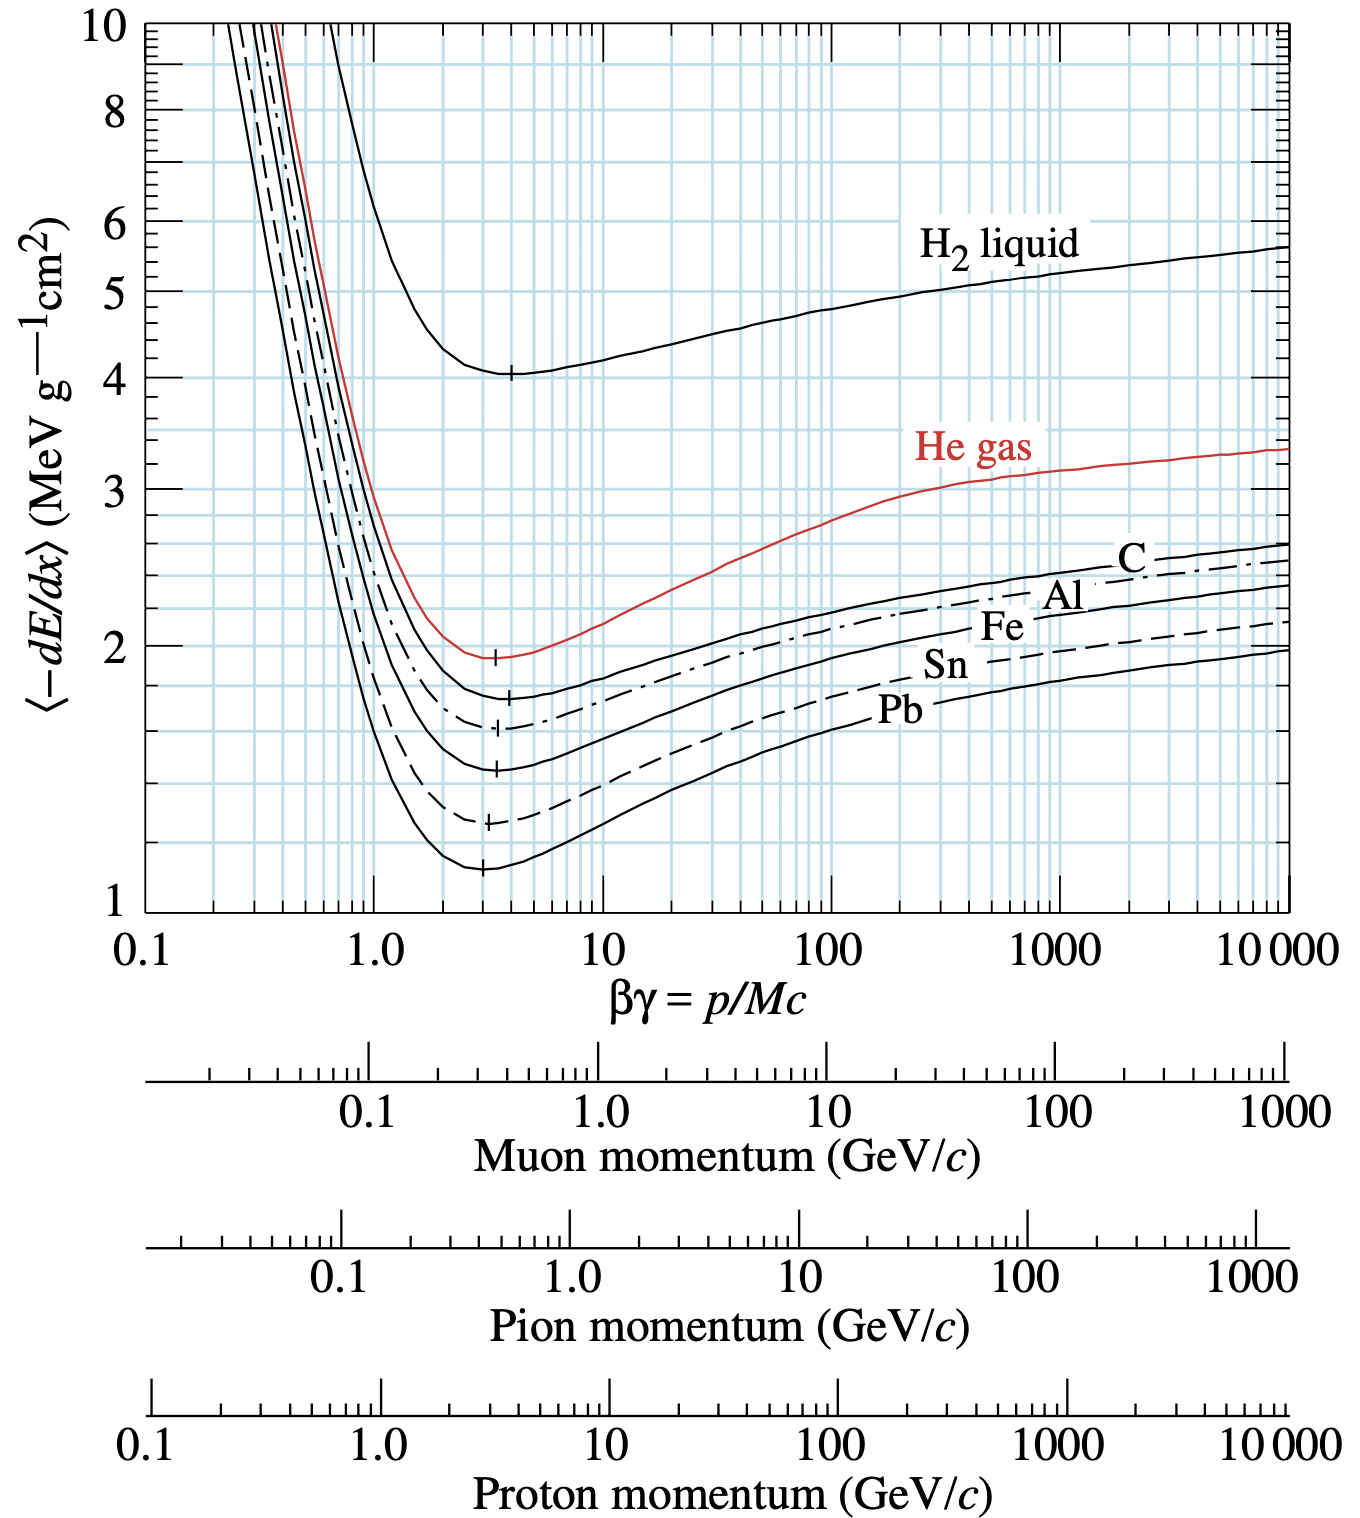
\includegraphics[keepaspectratio, scale=0.4]
 	{Figure/Siwecal/dedx.png}
 		\caption{水素(液体)、ヘリウム(気体)、炭素、アルミニウム、鉄、スズ、および鉛における平均エネルギー損失と、入射粒子(ミューオン、パイ中間子、陽子)の速度の関係。}
	\end{center}
 \end{figure}
\subsubsection{制動放射}
荷電粒子が物質を通過する際には電離の他に、原子核との衝突によって電磁波を放射しエネルギーを失うこともある。物質を構成する原子核はそれぞれ電場を持っており、電場によってRutherford散乱を受けた荷電粒子は加速、減速をされ、光子を放射しエネルギーを失う。これを制動放射(Bremsstrahlung)と呼ぶ。制動放射によって荷電粒子が失うエネルギー損失率は、
\begin{equation}
	\label{energyloss}
	- { \frac{dE}{dx} } = \frac{E}{L_R}
\end{equation}
$L_R$は放射長(Radiation Length)と呼ばれており、平均エネルギーがeの因子だけ小さくなる平均の長さを指す。$L_R$は以下のように与えられる。
\begin{align}
\frac{1}{L_R} = 4 {\left( \frac{\hbar}{mc} \right)}^2 Z (Z+1) {\alpha}^3 n_{\alpha} \ln(\frac{183}{Z^{1/3}})
\end{align}
式(\ref{energyloss})を積分することで、初期エネルギー$E_0$を持った荷電粒子が物質を$x$だけ進むときのエネルギー損失は以下のようになる。
\begin{equation}
E = E_0 \exp{-x/L_R}
\end{equation}
電離エネルギーと制動放射によって失うエネルギーの大きさが同じになる入射電子のエネルギーを臨界エネルギー$E_c$と呼び、この値よりもエネルギーが小さい場合はエネルギー損失がBethe-Blochの式に従い、大きい場合は制動放射によって主にエネルギーを失う。(臨界エネルギーは物質によって異なるがおおよそ$E_c \simeq 500[MeV] / Z$と表される。)荷電粒子の制動放射によって失われるエネルギーは質量の二乗に反比例するが、電離エネルギー損失は質量に強く依らない (図\ref{dE/dx})ため、ほとんどの粒子に対しては制動放射よりも電離損失が支配的となる。 一方で電子においては制動放射によるエネルギー損失が支配的であり、$E_c$は電磁カロリメータなどの設計において重要なパラメータとなる。
\subsection{光子}
電荷を持たない光子は物質中で電離は起こさず、主に図\ref{photon}に示す光電効果、コンプトン散乱、電子陽電子対生成の 3 つの過程で相互作用する。
\begin{figure}[H]
	\begin{center}
 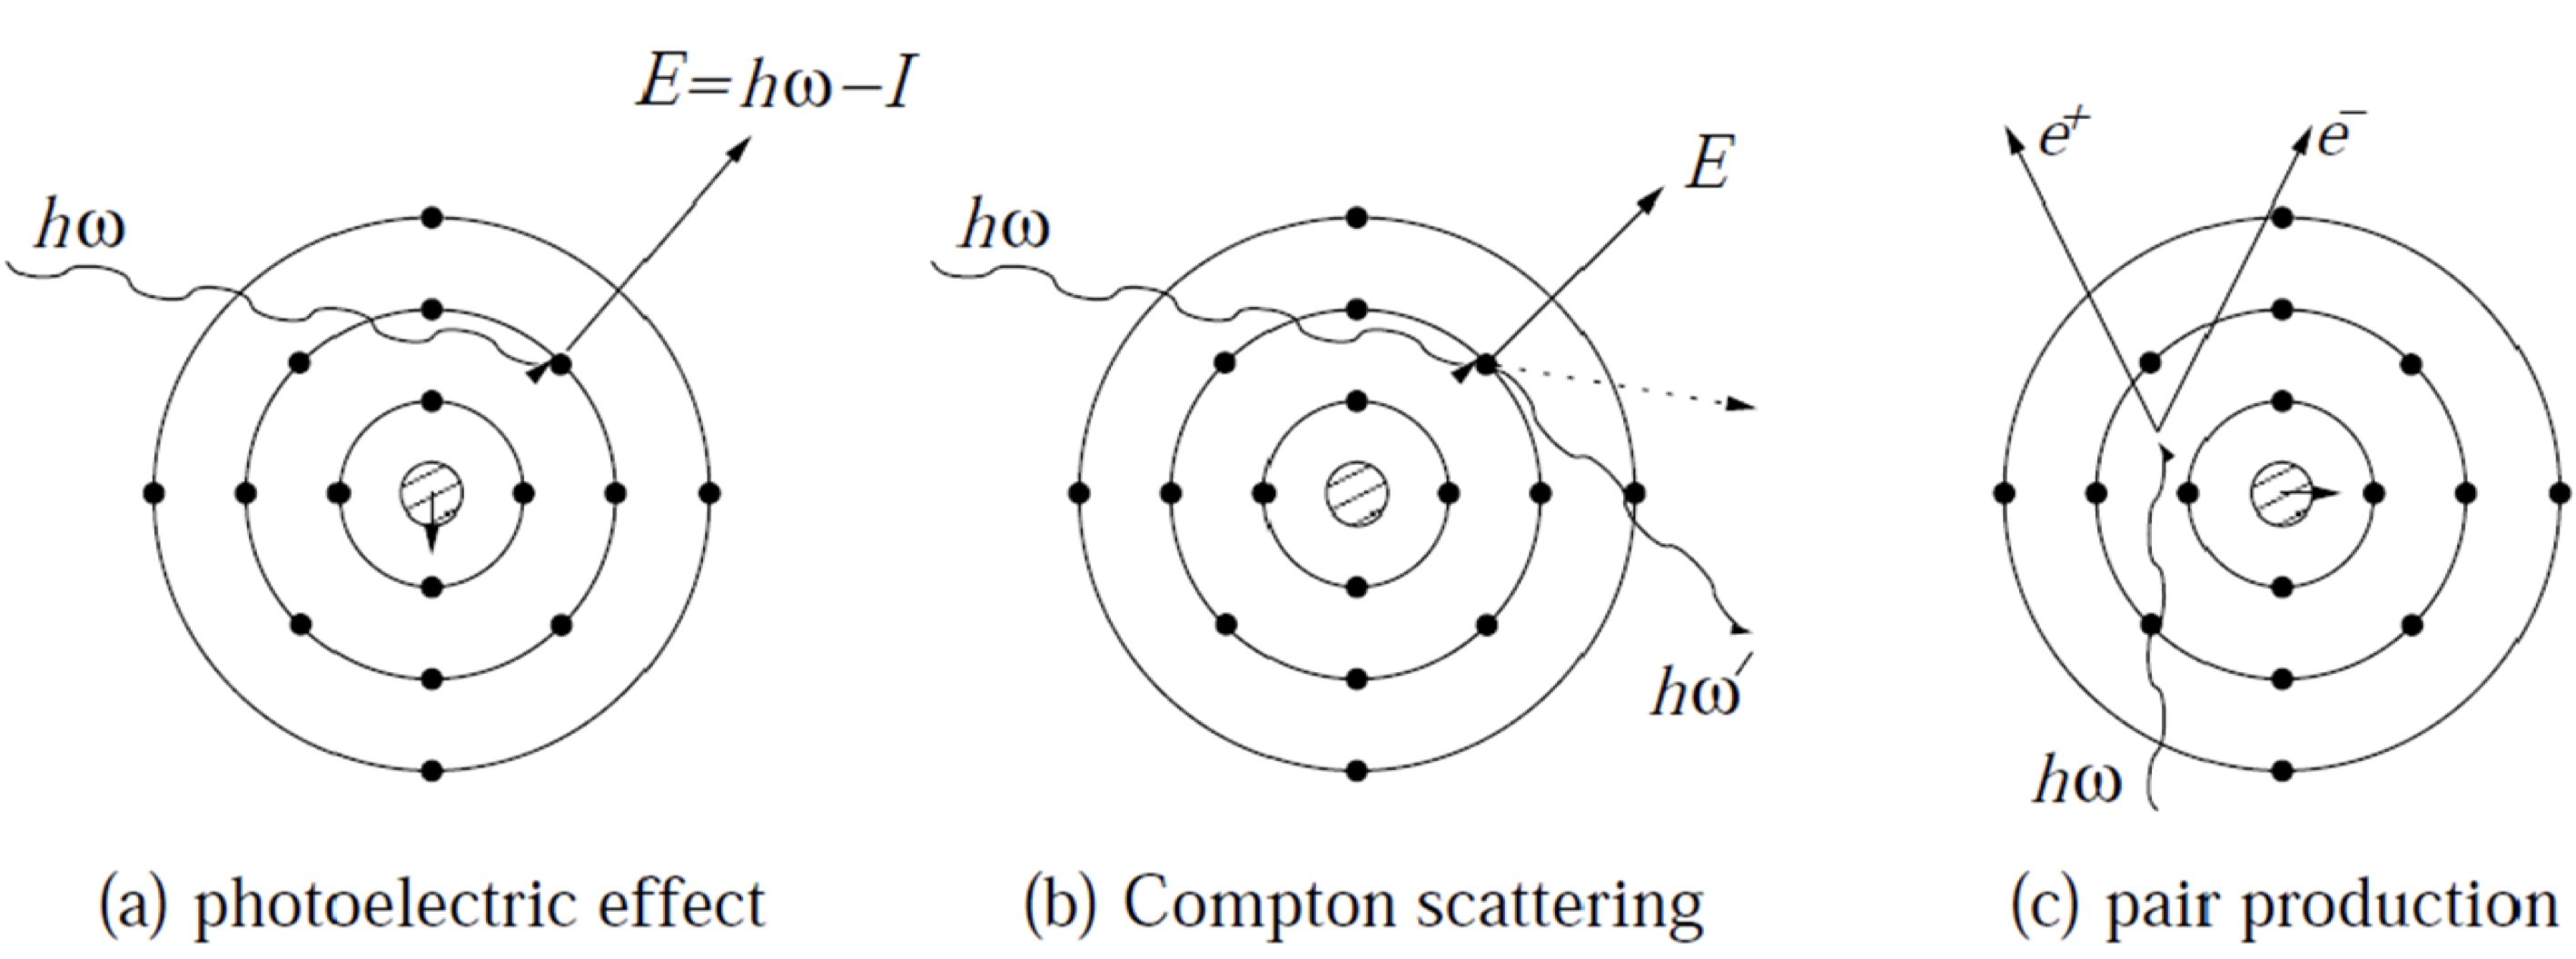
\includegraphics[keepaspectratio, scale =0.2]
 	{Figure/Siwecal/photon.png}
 		\caption{光子と物質の相互作用}
 		\label{photon}
	\end{center}
 \end{figure}
\begin{itemize}
 \item 光電効果 (Photoelectric effect): 入射光子が物質に当たることで光子の持っていたエネルギー$h\nu$が物質の電子に与えられる。これによって励起された電子が$h\nu - I$の運動エネルギーで飛び出す現象。($I$はイオン化エネルギー)
 \item コンプトン散乱 (Compton scattering): 入射光子と原子核に束縛されている1つの電子との弾性散乱。光電効果よりも光子のエネルギーが大きく、電子陽電子対生成反応よりも小さい時に支配的な反応である。
 \item 電子陽電子対生成 (Pair production): 入射光子が原子核のつくるクーロン場において消滅し、電子陽電子の対を生成する反応。この反応では、光子のエネルギーが電子陽電子の静止質量の和(およそ1.02MeV)よりも大きい必要がある。
\end{itemize} 
 光子のエネルギーによってこれらの反応確率は異なり、図\ref{photon_cs}に光子のエネルギーに対する各反応の確率を示す。中でも数MeV 以上の光子においては電子陽電子生成反応が主要なプロセスであり、ILCのような高エネルギーにおいては電子陽電子対生成が重要である。 物質に入射した光子は電子陽電子を生成し、さらに制動放射によって光子を放出する。これを繰り返すことで電子陽電子と光子の数が指数関数的に増加していき、この現象が電磁シャワーと呼ばれている。この時、電子陽電子対生成過程の断面積は$E_\gamma \gg mc^2/ \alpha Z^{1/3}$において
 \begin{align}
 \sigma_{pair} = \frac{7}{9}\frac{1}{n_a L_R}
 \end{align}
 と近似することができ、光子の飛程はおよそ$9/7L_R$となる。電磁シャワーは発展するにつれてエネルギーが下がり、臨界エネルギー(ILCの検出器ではおよそ10 MeV)に到達すると電子陽電子生成過程が起こらなくなり収束する。粒子のエネルギーを測定する場合には、シャワー内の荷電粒子をMIPとみなし、それらの粒子数が初めの光子のエネルギーに比例すると考えることで、検出器のセンサーに残したエネルギー損失の和をとることで測定する。\\
 また電磁シャワーは進行方向だけでなく垂直方向にも広がり、モリエール半径$R_M$によって広がりが測られる。モリエール半径とは、エネルギーの90$\%$が入るシャワーの半径を指し、以下の式で表される。
\begin{equation}
 \label{moliere}
 R_M \sim \frac{21 (\mathrm{MeV}) L_R}{臨界エネルギー (\mathrm{MeV})}  (\mathrm{g}/\mathrm{{cm}^2})
\end{equation}
\begin{figure}[h]
	\begin{center}
 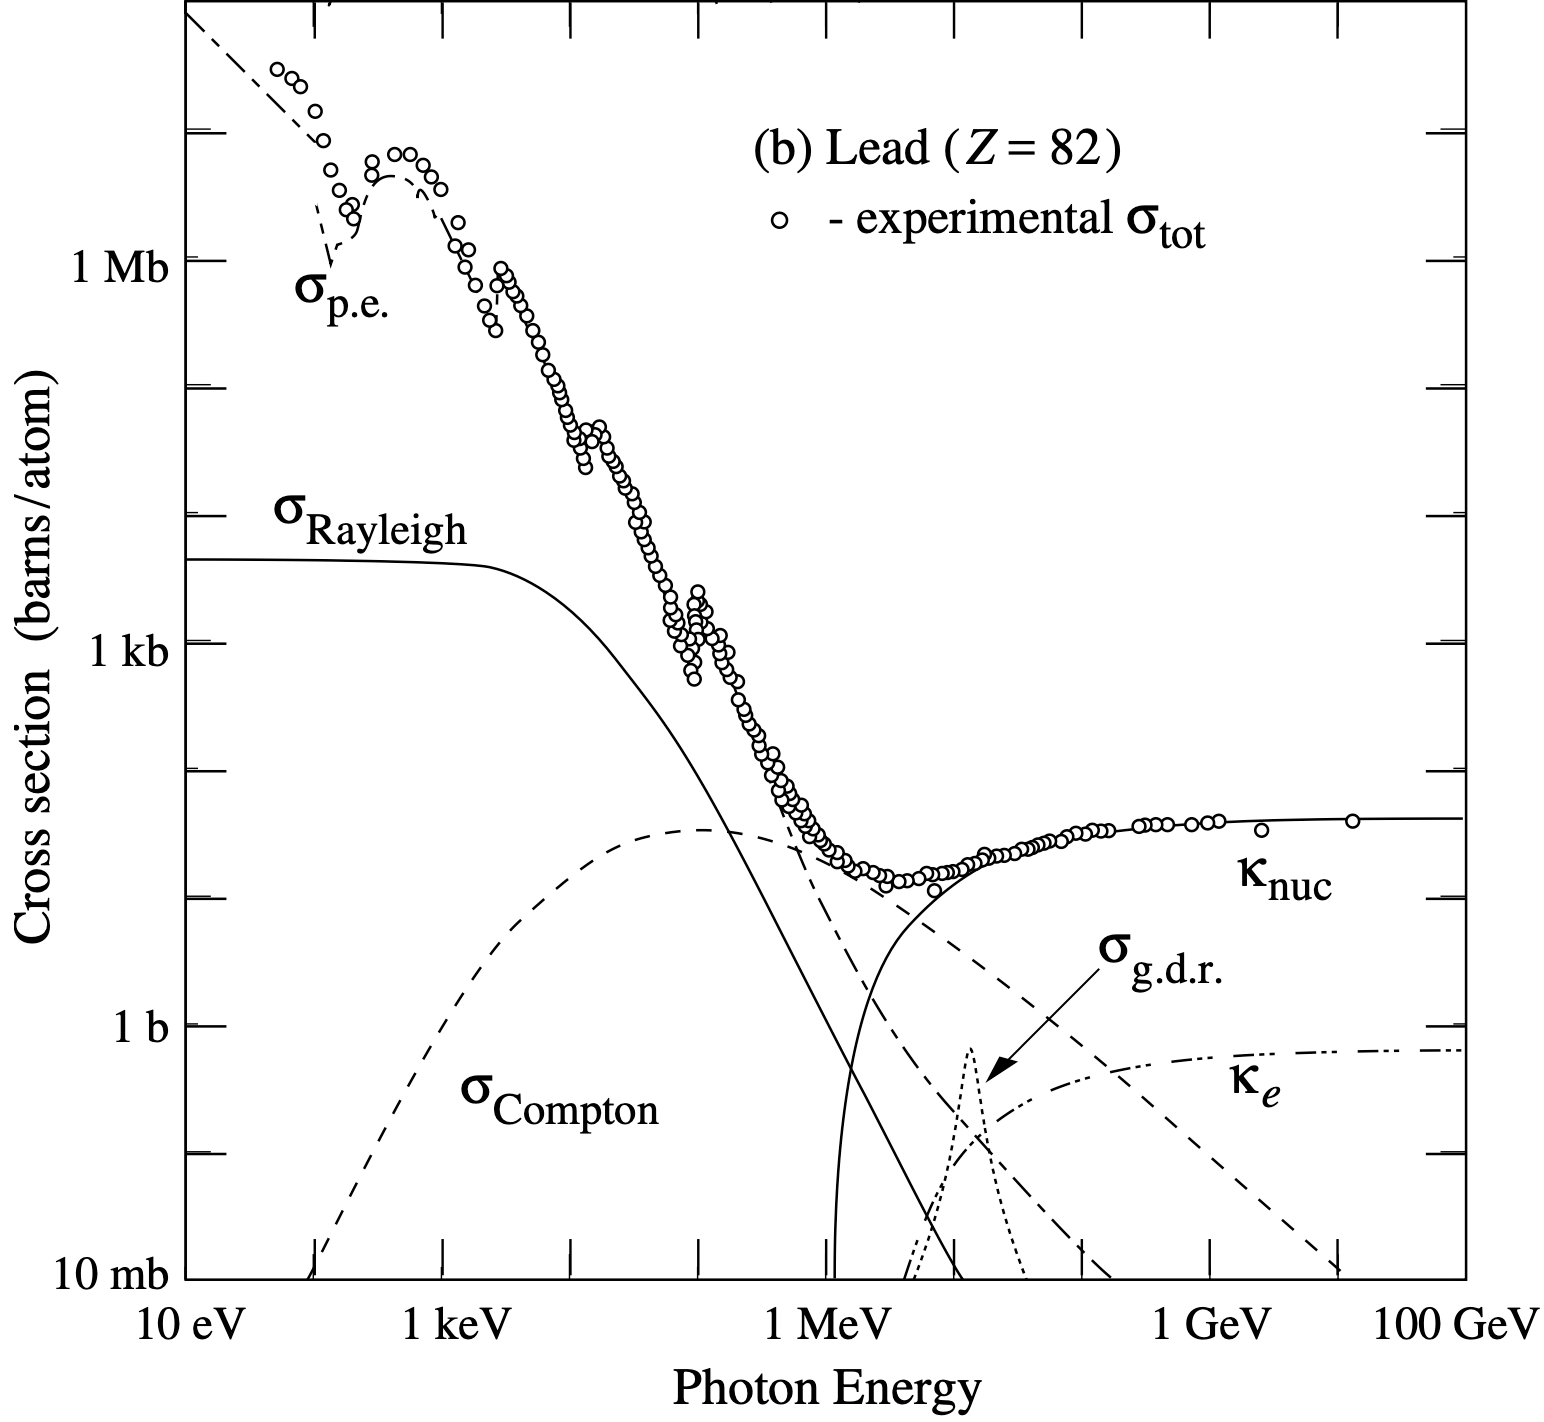
\includegraphics[keepaspectratio, scale=0.4]
 	{Figure/Siwecal/photon_crosssection.png}
 		\caption{光子と鉛の相互作用における断面積と光子のエネルギーの関係。${\sigma}_{p.e.}$は光電効果を、${\sigma}_{Compton}$はコンプトン散乱を、${\kappa}_{e}, {\kappa}_{nuc}$は電子陽電子対生成を指す。}
 		\label{photon_cs}
	\end{center}
 \end{figure}
\subsection{ハドロン}
$\pi$中間子やK中間子などのハドロンは物質を構成する原子核と衝突し、非弾性散乱を繰り返すことでハドロンシャワーを生成する。ハドロンの相互作用長は典型的に放射長よりも大きく、ハドロンをカロリメータで測定する場合には非常に多くの物質を必要とする。相互作用長は以下のように表される。
\begin{align}
\lambda = \frac{A}{N_a \rho} \sigma_{total}
\end{align}
ここで、$\rho$は物質の密度を、$ \sigma_{total}$は反応断面積の総和を表す。ハドロンシャワーには${\pi}^0 \rightarrow \gamma \gamma$崩壊によって発生する電磁シャワーが混ざってしまっており、検出器のエネルギー応答が異なることから、ハドロンシャワーのエネルギー分解能は電磁シャワーと比較して非常に悪くなってしまう。
\section{粒子検出器の動作原理}
 素粒子実験では、前節の相互作用を用いて粒子を検出する。粒子の検出には、事象を区別するために十分な時間分解能と位置分解能を持つ必要があり、また各粒子を識別するために、エネルギーと運動量を十分な精度で測定する必要がある。以下では、測定器を構成する検出器のうち特に重要なものを取り上げる。
\subsection{ガス検出器}
 ガス検出器は、主にアルゴンのような活性の低いガスを検出器内に充填した検出器である。荷電粒子がガス中を通過することで電離反応を起こし、生成される電子と陽イオンを電極に集める、あるいは電離の軌跡を可視化することで荷電粒子を検出することができる。主な検出器としては、電極への印加電圧が小さい領域では電離箱が、大きい領域ではワイヤーチェンバーや抵抗板チェンバー(RPC)などが挙げられる。
\subsection{半導体検出器}
 半導体検出器とは半導体材料を使用した検出器を指し、光や電子をはじめとして様々な粒子を検出するものがある。半導体材料には主にシリコンやゲルマニウムが用いられ、接合ダイオードの原理を使用して製造される。以下では、シリコン検出器の構造と動作原理について説明する。まず基本構造としては、検出器の一方に正孔の多いp型半導体、もう一方の面に自由電子が多いn型半導体のp-n接合が作られてある。それぞれに対して逆バイアス電圧(p型に負、n型に正)を印加することで、p型とn型との間で正孔と自由電子の結合が進み、空乏層と呼ばれる安定化した領域が検出器の接合面を中心に広がる。この空乏層を通過した荷電粒子は、検出器内のシリコン原子を励起し、電子正孔対を生成する。飛跡に沿って生成された電子正孔対は、空乏層内の電場によって両印加極板までドリフトされ、パルス電流として測定される。また、シリコンなど半導体のバンドギャップは1eV程度であり、電子正孔対を生成するために必要なエネルギーはおよそ$3,4$eVとなっている。この信号の小ささから、半導体検出器では読み出しにおいて増幅を必要とするため、増幅回路が近傍(あるいは半導体内部)に存在している。半導体検出器は、電極が平面構造のピクセル検出器や帯状のストリップ検出器、検出器基板上に増幅回路を形成するモノリシック検出器など、電極や増幅回路の実装によって様々な構造が存在する。
\subsection{シンチレーション検出器}
 励起エネルギーの一部が、より低いエネルギー準位へ遷移する際に可視光として表れる物質をシンチーレタという。シンチレータ検出器は、荷電粒子の通過によって発生した蛍光(シンチレーション光)を光検出器によって測定することで動作する検出器である。シンチレーション光は非常に弱い光信号であるため、検出においては光電子増倍管を用いて信号を増幅し検出する。
 
\section{シリコンタングステン電磁カロリメータ SiW-ECAL}
\subsection{SiW-ECALの全体構造}
ILDのSiW-ECALは、図\ref{SiW-ECAL}のようにタングステンの吸収層とシリコンパッドセンサーの検出層が、30層サンドウィッチ状に交互に重なったサンプリング型カロリメータである。1つのモジュールが10ほどのサブモジュールに分かれており、サブモジュールにはそれぞれ4枚のシリコン半導体センサーが貼り付けられる。
\begin{figure}[h]
 \begin{minipage}[h]{.45\linewidth}
	\begin{center}
 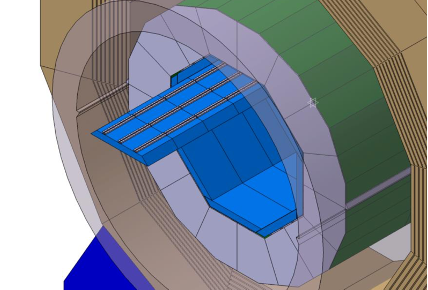
\includegraphics[keepaspectratio, scale=0.8]
 	{Figure/Siwecal/ECAL.png}
 		\caption{ILDおよびECALの全体図}
 		\label{ECAL}
	\end{center}
\end{minipage}
\hfill
\begin{minipage}[h]{.45\linewidth}
	\begin{center}
 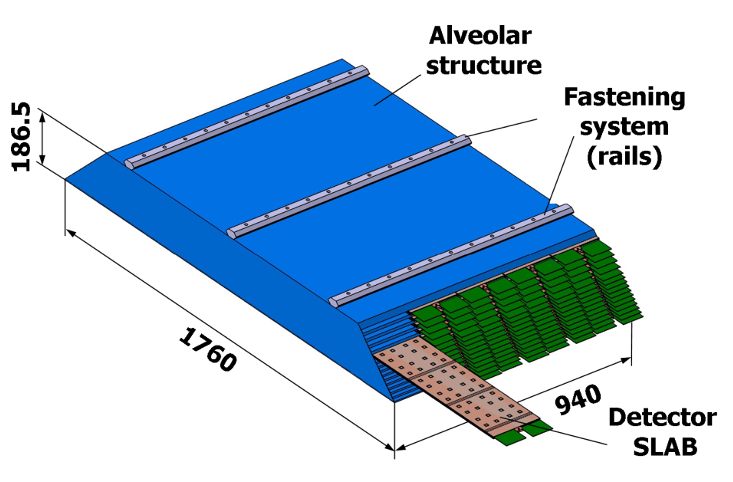
\includegraphics[keepaspectratio, scale=0.8]
 	{Figure/Siwecal/SiW-ECAL.png}
 		\caption{SiW-ECALの構造}
 		\label{SiW-ECAL}
	\end{center}
\end{minipage}
\end{figure}

\subsection{シリコン半導体検出器}
SiW-ECALでは検出層にシリコン半導体検出器を用いる。センサーの大きさは1枚あたり$9 \times 9 {cm}^2$で、1枚に$5.5 \times 5.5 {mm}^2$のピクセルが$16 \times 16$個並んでおり、1つサブモジュールあたり1024チャンネル読み出しが可能となっている。またシリコンセンサーには、電極としてアルミニウム ($Al$) 、絶縁層に二酸化ケイ素 ($SiO_2$)が使用される。 厚さ320$\mu m$のセンサーでは、1MIPあたり86.8keVのエネルギー損失が起こり、臨界エネルギーに達するまでに生成される電子正孔対はおよそ24,000、電荷にして4fCとなる。シリコンセンサーは、常温硬化型導電性接着剤によって回路基板(PCB)と接着されており、PCBを通して信号の読み出しが行われる。以下にセンサーの仕様と1枚のシリコンセンサーパッドを示す。
\begin{figure}[H]
 \begin{minipage}[h]{.45\linewidth}
 \def\@captype{table}
   \centering
   \caption{シリコンセンサーの仕様}
   \begin{tabular}{|c|c|}
         \hline
   	制作会社 & 浜松ホトニクス株式会社\\
	サイズ & 89.7 $\times$ 89.7 $\mathrm{{mm}^2}$ \\
	セルサイズ & 5 $\times$ 5 $\mathrm{{mm}^2}$\\
	セル数 & 16 $\times$ 16 = 256\\
	厚さ & 320/500/650$\mu m$\\
	完全空乏化電圧 & 40/70/110 V\\
        \hline
  \end{tabular}
\end{minipage}
\hfill
\begin{minipage}[h]{.45\linewidth}
	\begin{center}
 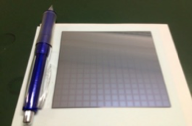
\includegraphics[keepaspectratio, scale=0.8]
 	{Figure/Siwecal/si_sensor.png}
 		\caption{シリコンパッドセンサー}
 		\label{sensor}
	\end{center}
\end{minipage}
\end{figure}
\subsection{読み出しシステム}
 SiW-ECALは高精細であることから読み出しチャンネル数が非常に多くなっており、30層のECAL全体ではおよそ1億にもおよぶ。そのため、シリコンセンサーからの信号読み出しをコンパクトにする必要があり、読み出し専用のASIC(Application Specific Integrated Circuit)が開発された。現在の技術プロトタイプに実装されているASICには、フランスのOmegaグループが開発したSKIROC(Sillicon Kalorimeter Integrated ReadOut Chip)シリーズの第二バージョンであるSKIROC2Aを用いている。\\
 まず、読み出しに用いるASICに求められる性能には次に挙げる項目が求められる。
 \begin{itemize}
	\item 自動トリガー:\\
		信号に対してASIC自身でトリガーをかける。
	\item 完全デジタル出力:\\
		 シリコン半導体検出器からのアナログ情報をすべてデジタル変換し、DAQへ送信する。データ量を圧縮し、またデータの劣化を防ぐことができる。
	\item 発熱量の抑制 :\\
		電力消費によって発生するジュール熱を、1チャンネルあたり25$\mu W$ 以下に抑える。
	\item 1 MIP 相当の信号を識別できる高い Signal to Noise 比 (S/N 比):\\
		PFAにおいてジェットエネルギー分解能を向上させるために、高い精度で粒子を識別する必要がある。
 \end{itemize}
 続いて、SKIROC2Aの基本的な仕様を以下に示す。
 \begin{itemize}
 	\item Austria Micro Systems社製 0.35 $\mu m$ SiGe
	\item 7.5 $\times$ 8.5 ${mm}^2 /1チップ$
	\item 1チップあたり64チャンネル読み出し可能
	\item 2種類のダイナミックレンジをもつADC (Analog to Digital Converter) mode :\\
		電磁シャワー内の粒子が1つのチャンネルに大量に入射したときに全エネルギーを測定出来るよう、幅広いゲインのレンジを持つ。
		\begin{itemize}
			\item High gain \ldots \ 0.5 $\sim$ 150 MIP 相当の信号に対応
			\item Low gain \ldots \ 150 $\sim$ 2500 MIP 相当の信号に対応
		\end{itemize}
	\item TDC (Time to Digital Converter) mode : 1ns程の時間分解能で時間情報を保存
	\item 1チャンネルあたり15イベント保持可能なAnalog memory cell\\
		ビームバンチ構造に対応するため、200nsの間イベントを保持することが可能。1つのMemory cellでは、High gain ADC、Low gain ADCを、時間情報であるBCID (Bunch crossing ID) と紐づけて保存。
	\item 数珠つなぎ型読み出し : 順番に読み出すことで読み出していないチップの電源を必要とせず、消費電力を減らす
	\item 0.5 MIPでの自動トリガー
	\item 全64チャンネルの閾値を個別で同時設定可能な10 bit DAC threshold
	\item Power pulsing mode
 \end{itemize}
データ収集の手順は、以下のとおりである。まずシリコンセンサーからのアナログ信号が各チャンネルに入力され、前置増幅器によって前段増幅を行う。ここでの増幅率は、前置増幅器のfeedback capacitanceによって変更可能となっており、増幅率が最大となる0pFから6.0pFまで0.4pF刻みで決定することができる。前段増幅を経た信号は、Fast shaperと2つのSlow shaper(Low/High gain)の3つに分割される。Fast shaperに入った信号は、CRRC shaperによって信号をさらに増幅したのち、discriminatorにて閾値を超えた場合のみトリガー信号を出し、同時に入ってきたSlow shaperの信号電圧をMemory cellに保持する。ここで、CRRC shaperとは微分回路と積分回路を組み合わせた回路であり、信号増幅率と立ち上がり時間を調整している。Memory cell に保持されたchargeは、読み出し時間が経過、あるいはMemory cellが満たされたタイミングでマルチプレクサー(MUX)に送られる。一方、Slow shaperにおいても信号がCRRC shaperによって増幅率1、10倍に増幅され、トリガー信号によってMUXに送られる。MUXでは、Slow shaper(Low or High)とTDCの組み合わせを決定し、wilkinson型12bit ADCによってアナログ信号をデジタル化し、メモリに保存されたのち外部へ転送される。図\ref{skiroc2a}にSKIROC2Aのアナログ部の回路図を示す。
\begin{figure}[H]
	\begin{center}
	\includegraphics[keepaspectratio, scale=0.7]
% 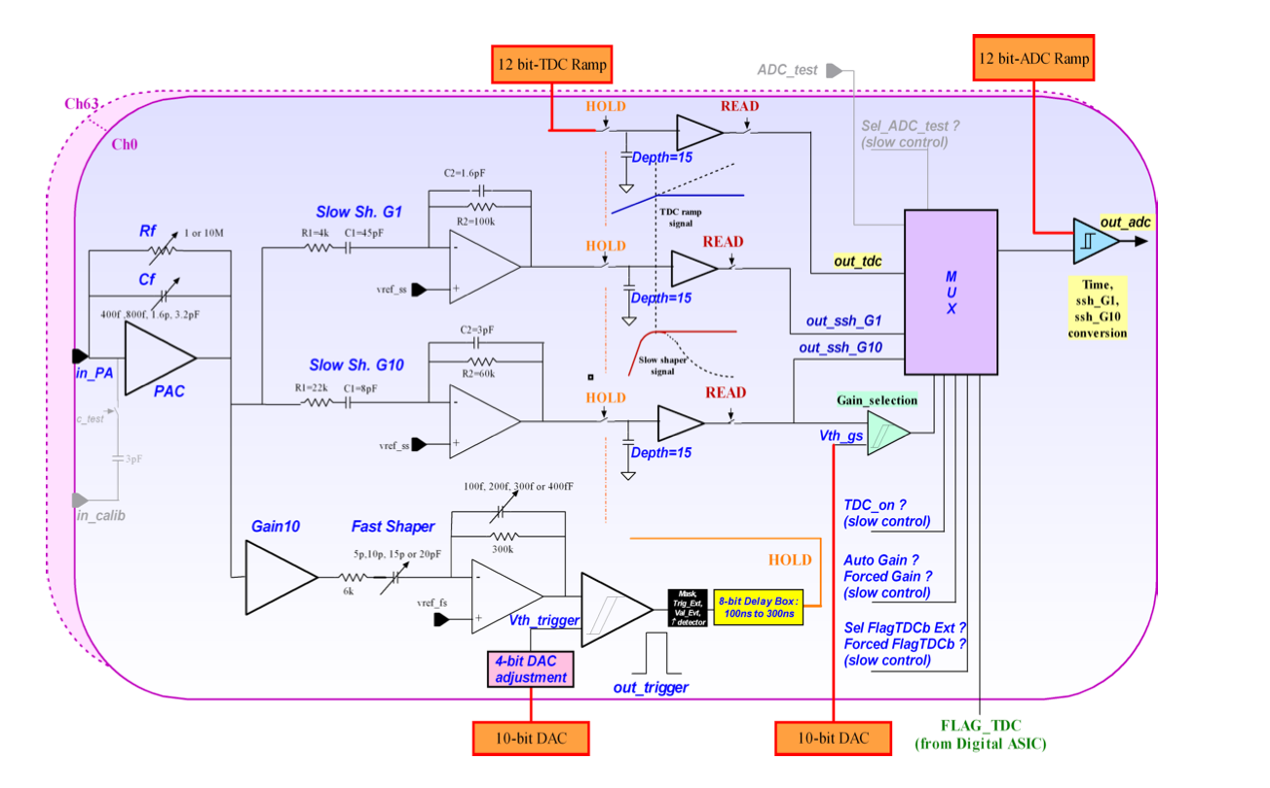
\includegraphics[width=\linewidth,angle=90, scale=1.5]
 	{Figure/Siwecal/skiroc2A.png}
 		\caption{SKIROC2Aのアナログ部の回路図}
 		\label{skiroc2a}
	\end{center}
 \end{figure}

\subsection{タングステン吸収層}
ILDのSiW-ECALの吸収層ではPFAの要件を満たすために、相互作用長が長く放射長の短い物質でシャワーの広がりを小さく抑える物質を採用する必要がある。そのため、モリエール半径が小さく、放射長に比べ相互作用長が大きいタングステンが採用されている。表\ref{metal}に物質量が大きく吸収層の候補となる物質の性質について示す。
\begin{table}[h]
 \centering
  \begin{tabular}{c||ccc}
   \hline
   物質 & $\lambda/cm$ & $L_R/cm$ & $R_M/cm$ \\
   \hline \hline
	鉄 & 16.8 & 1.76 & 1.69\\
	銅 & 15.1 & 1.43 & 1.52\\
	タングステン& 9.6 & 0.35 & 0.93\\
	鉛 & 17.1 & 0.56 & 1.00\\
   \hline
  \end{tabular}
   \caption{物質量の大きい吸収層の候補物質($\lambda$は相互作用長、$L_R$は放射長、$R_M$はモリエール半径を示す。)}
   \label{metal}
\end{table}
\subsection{技術プロトタイプ}
SiW-ECALの技術プロトタイプとして、図\ref{shortslab}のような構造が考えられている。図\ref{shortslab}は、1層の検出器 (Slab) の一部として作製されたShort slabである。図の上から構造体として炭素繊維強化プラスチック (CFRP) の板があり、その下に読み出し基板(FEV)やASICの制御基板があり、基板下にはセンサーに接触し電荷を印加する導電性シートがあり、さらにカーボンの板で挟まれている。1層あたり、FEVにはPCB上にSKIROC2Aが16チップ実装されており、裏面にはシリコンパッドセンサー4枚が導電性接着剤で接着されている。また、ASICはFPGAを通して制御されており、さらに図\ref{core}のようなモジュールを通して、複数のSlabからの信号を同時に読み出している。この技術プロトタイプの開発は、フランスと日本を中心にCALICEグループによって国際協力で行われており、国内においてもモジュールの生産・組み立ては可能となっている。
\begin{figure}[h]
	\begin{center}
	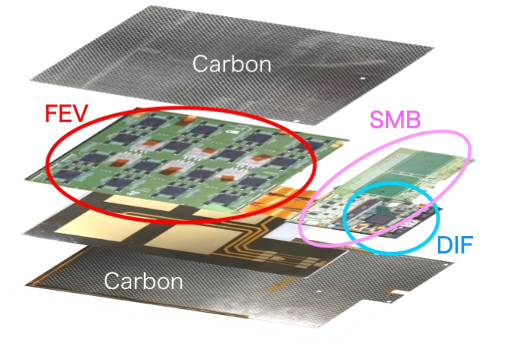
\includegraphics[keepaspectratio, scale=0.7]
 	{Figure/Siwecal/shortslab.png}
 		\caption{short slabの構造}
 		\label{shortslab}
	\end{center}
 \end{figure}
 \begin{figure}[h]
	\begin{center}
	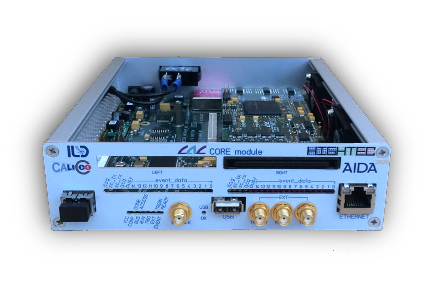
\includegraphics[keepaspectratio, scale=0.7]
 	{Figure/Siwecal/core.png}
 		\caption{多層読み出しのためのCOREモジュール}
 		\label{core}
	\end{center}
 \end{figure}
 % !TEX root = ../MasterThesis_Onoe.tex
% 上記はただのコメントではなく親ファイルの場所を教えているので
% 消してしまうとファイルごとのタイプセットができなくなるので注意。
% 親ファイル名を変更したときはここも変更する。

\chapter{ビームテストによる評価試験} \label{sec:Beamtest}
これまでに作成されたSiW-ECALの技術プロトタイプ(FEVおよびCOB)の性能評価実験を、2023年6月7日から2023年6月22日の期間にCERN SPS加速器のビームラインにて行った。本実験の主な目的は、電磁カロリメータとハドロンカロリメータの技術プロトタイプを同じビーム軸上に設置し、同時に運転を行いデータを取得すること、またこれまでの評価実験の中でも最高エネルギーのハドロンビームを用いて15層のSiW-ECALの評価を行うことの2点であった。また本実験におけるハドロンカロリメータは、同じくCALICEグループにおいてドイツやチェコが中心となって開発を進めているAHCALを用いた。以下では実験の詳細と、結果について述べる。
\section{ビームライン}
ビームテストは、フランスとスイスの国境付近に位置するCERNのSPS 加速器のビームラインを用いて行った。SPSは、現在 LHC の前段加速器として利用されており、陽子シンクロトロンから来た$\SI{26}{GeV}$の陽子を、周長7kmの加速器によって$400\sim \SI{450}{GeV}$まで加速している。SPSのビームラインでは、陽子ビームを固定ターゲットに入射することで、電子、ミューオン/パイ中間子の2次ビームを運動量$10\sim \SI{400}{GeV}$で得ることができる。本実験ではこれらのビームを用いて、NorthエリアにあるH2Aビームラインで実験を行った。実験に用いたビームパラメータを表 3.1に示す。\\
\begin{figure}[H]
	\begin{center}
 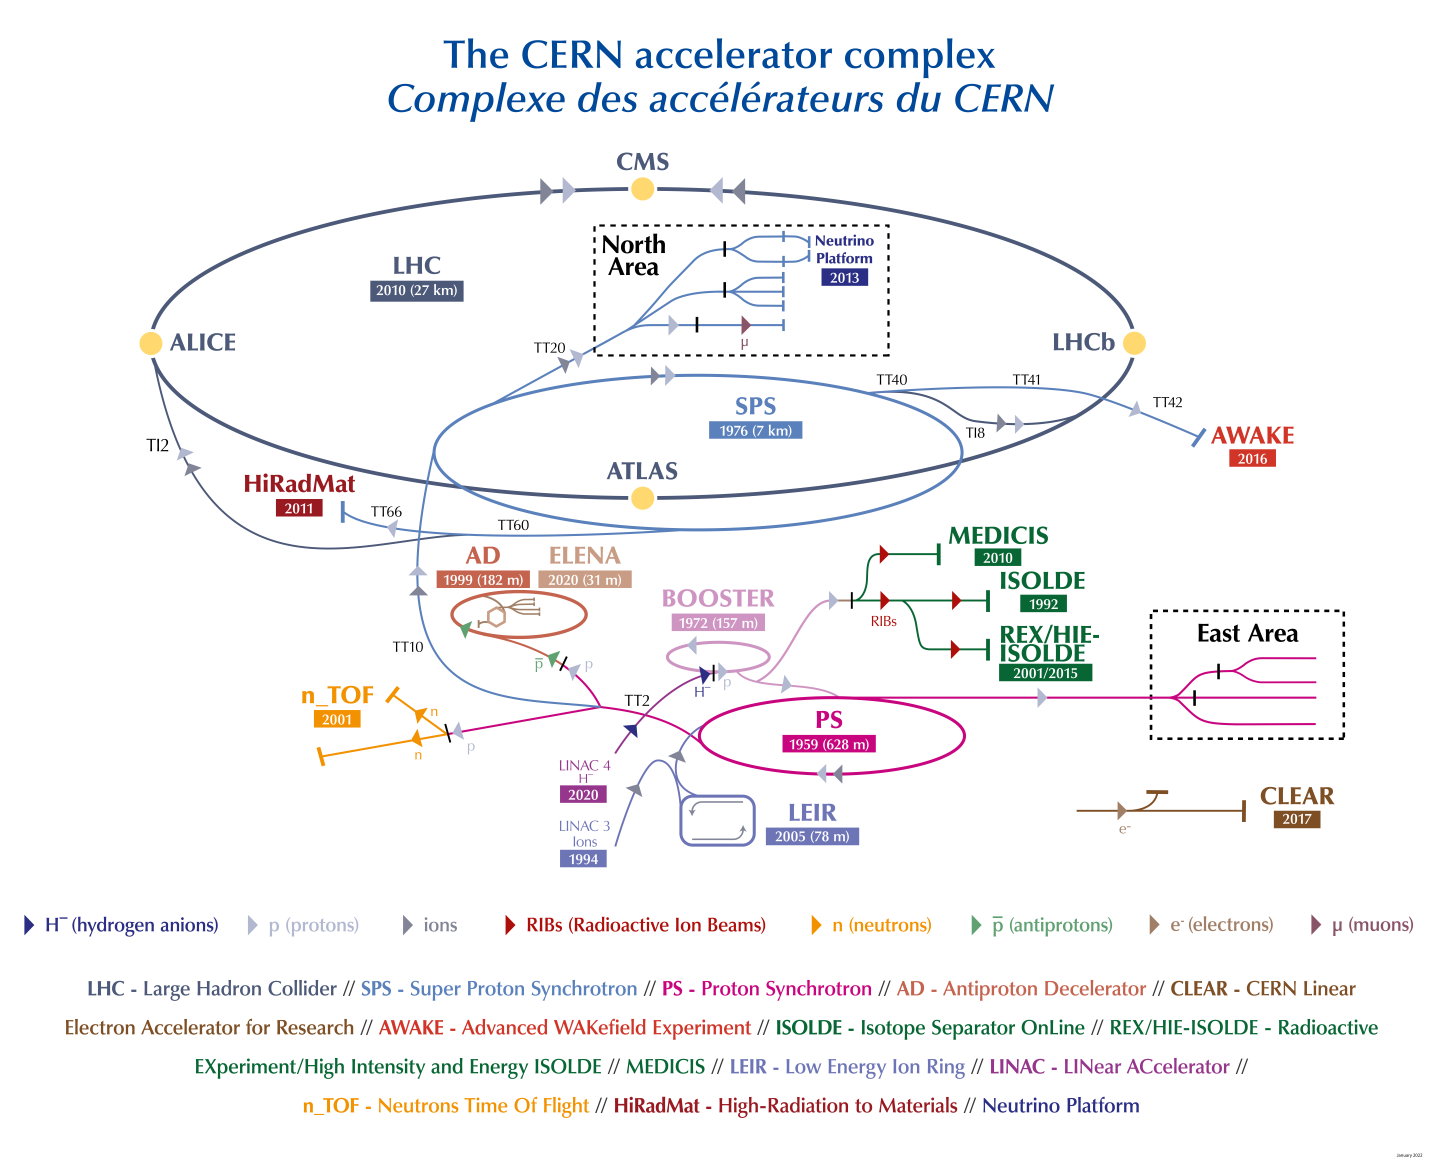
\includegraphics[keepaspectratio, scale=0.7]
 	{Figure/Beamtest/cern.png}
 		\caption{CERNの全体図}
	\end{center}
\end{figure}
\begin{table}[H]
 \centering
 \begin{tabular}{c c}
 \hline
運動量 & 10-200$[ \mathrm{GeV}/ c ]$\\
電子のpurity & 10-99.5\%\\
Max $\delta p / p$  & $2\%$\\
ビームの高さ & 2460$[ \mathrm{mm}]$\\
 \hline
 \end{tabular}
 \caption{H2Aビームラインにおけるビームパラメータ}
\end{table}

\section{実験セットアップ}
\subsection{測定機器のセットアップ}
本実験でのセットアップの概観を図\ref{setup1}に示す。図中右手からビームが照射され、ILDの構成と同様に上流側にSiW-ECALが、下流側にAHCALを設置した。SiW-ECALのプロトタイプは、FEVが13層(うちFEV10が1層、FEV11が3層、FEV12が2層、FEV13が7層)COBが2層を組み合わせた計15層からなる検出層と鉛板15層の吸収層からなるモジュールを組み立てた。今回のビームテストの検出層は、最も良い性能が期待できるFEV13を前方に設置し、性能比較のためにCOBを加えた構成となった。15層の検出層において、センサーと読み出しボードに供給する電源は、15層に対して図\ref{setup2}左のように並列で印加した。また、信号はカプトンケーブルを通して15層分の信号を一括してCOREモジュールに送り、PCで読み出しを行った。また、AHCALもサンプリング型ハドロンカロリメータであり、鉄の吸収層とシンチレータ検出層によって構成されていて、読み出しはシンチレータに統合されたエレクトロニクスによって行われる。
\begin{figure}[H]
\begin{center}
 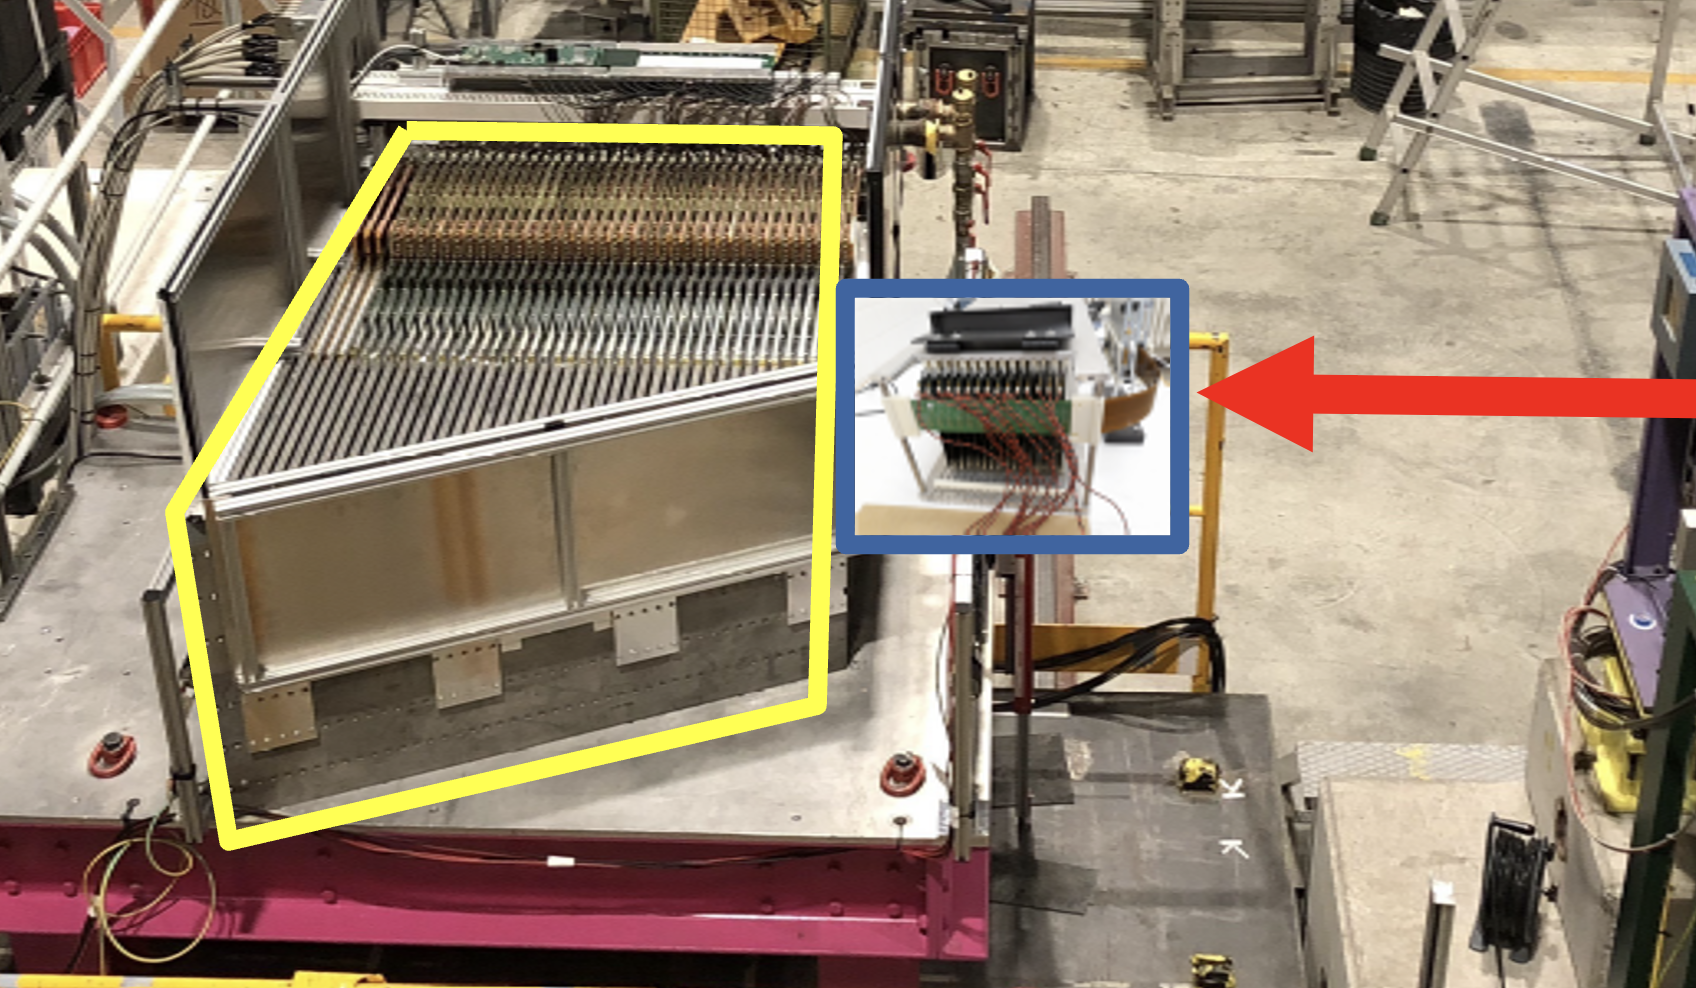
\includegraphics[keepaspectratio, scale=0.3]
 	{Figure/Beamtest/setup1.png}
 		\caption{セットアップの全体図。黄枠:AHCAL、青枠:SiW-ECAL、赤:ビーム位置}
		\label{setup1}
		\end{center}
\end{figure}

\begin{figure}[H]
\begin{center}
 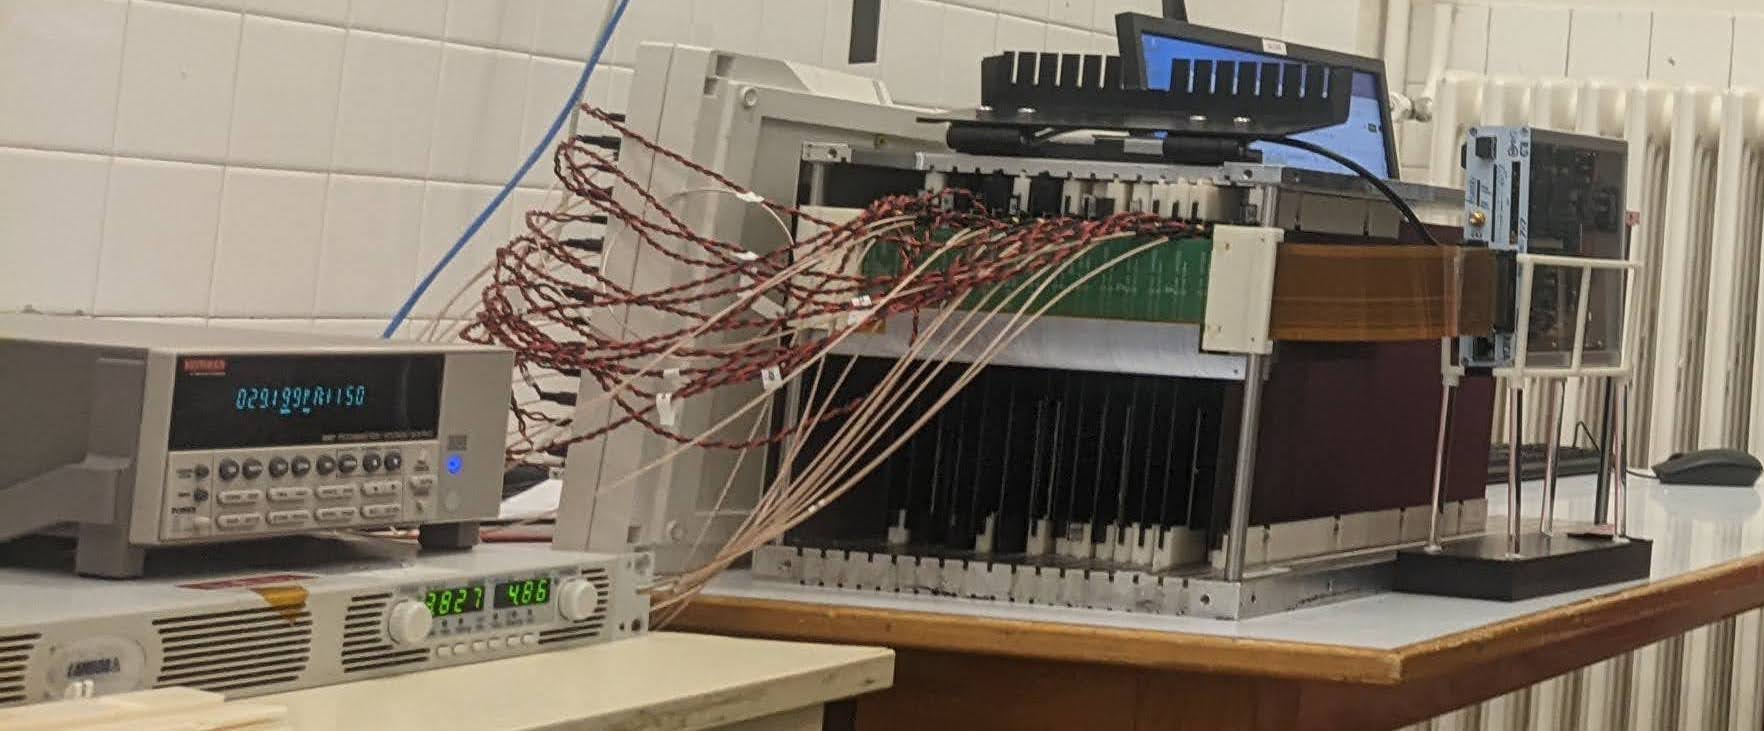
\includegraphics[keepaspectratio, scale=0.2]
 	{Figure/Beamtest/setup2.png}
 		\caption{SiW-ECALのプロトタイプモジュールと電源供給、読み出しシステム}
		\label{setup2}
\end{center}
\end{figure}

\begin{table}[H]
 \centering
 \begin{tabular}{|c|c|c|c|}
 \hline
層数 & ボードの種類 & ウェハー厚み$[\mu m]$ & タングステン厚み[mm]\\
 \hline
 \hline
0 & FEV13 & 650 & 4.2\\
1 & FEV13 & 650 & 4.2\\
2 & FEV13 & 650 & 4.2\\
3 & FEV13 & 650 & 4.2\\
4 & FEV13 & 500 & 4.2\\
5 & FEV13 & 500 & 4.2\\
6 & COB & 500 & 4.2\\
7 & FEV12 & 500 & 4.2\\
8 & COB & 500 & 5.6\\
9 & FEV12 & 500 & 5.6\\
10 & FEV11 & 320 & 5.6\\
11 & FEV11 & 320 & 5.6\\
12 & FEV10 & 320 & 5.6\\
13 & FEV13 & 320 & 5.6\\
14 & FEV11 & 320 & 5.6\\
 \hline
 \end{tabular}
 \label{layer}
 \caption{SiW-ECALのレイヤー構成 (0層目がビーム上流側) }
\end{table}
\subsection{信号読み出し}
ECALとHCALは独立にDAQを行うが、本実験ではEUDAQという読み出しフレームワークによってHCALと同期した読み出しを行った。EUDAQでは、ECALとHCALの間でClock and Control Card (CCC) を同期させており、CCCではクロック、スタート、ストップ信号をPCへ送っているため、PC上で時間情報である Bunch Crossing ID (BCID) が同じイベントを収集することができる。\\
また、ECALでは専用のDAQソフトウェア\cite{ecalsoft}が稼働しており、DAQのみでなくチャンネル単位での閾値の設定やイベントのモニター (図\ref{monitor}) が可能となっている。データはraw形式で保存され、解析用のソフトウェアを通してツリー形式にデータを保存したrootファイルへ変換し解析に利用することができる。
\begin{figure}[H]
\begin{center}
 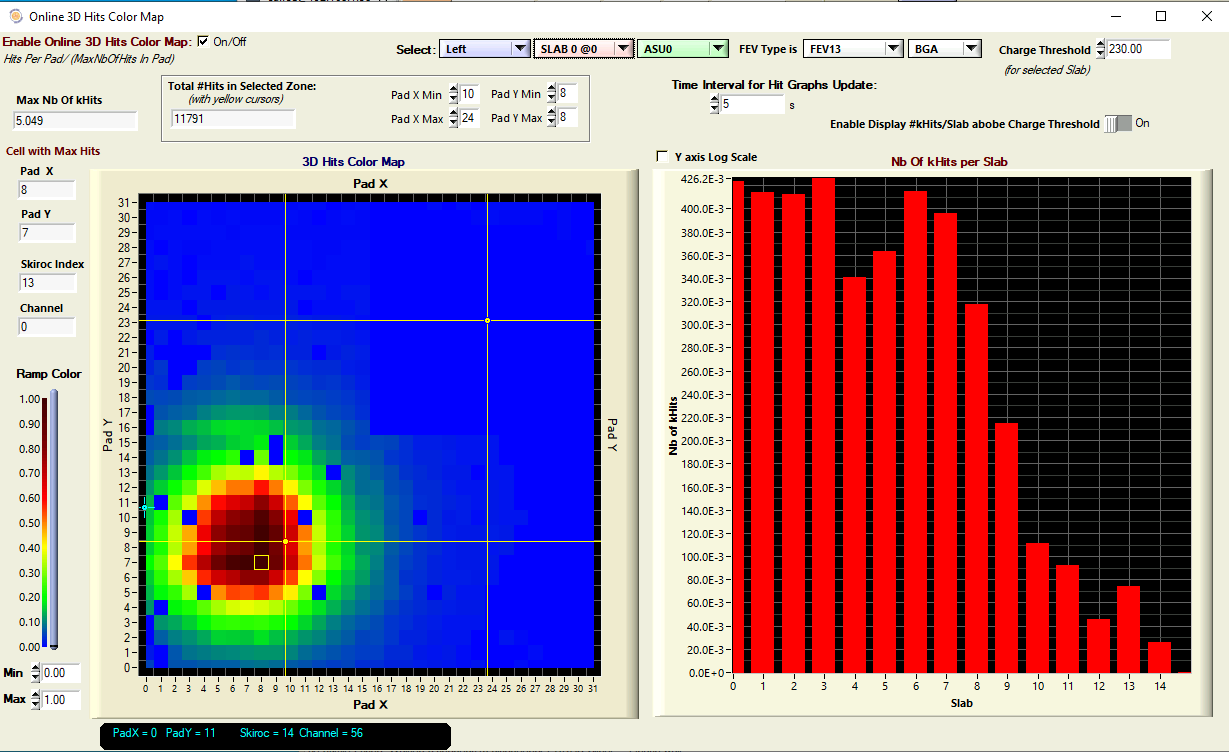
\includegraphics[keepaspectratio, scale=0.2]
 	{Figure/Beamtest/monitor.png}
 		\caption{SiW-ECAL読み出しソフトウェアにおけるイベントモニター (左) ヒットマップ (右) 各層あたりのヒット数}
		\label{monitor}
\end{center}
\end{figure}
\section{実験結果}
\subsection{検出器応答}
各runに対して層ごとのヒットマップを作成し、各層の応答を確認した。作成したヒットマップが図\ref{hitmap}である。ビームはヒットマップ左下のセンサーを中心に照射を行った。\\
電子ビームは相互作用を起こし電磁シャワーを形成するため、ヒット領域が大きくなっていることが確認できる。またミューオンビームは、電子ビームと比較して相互作用を起こさず、ビームサイズが小さい。また白く抜けている箇所はノイズが多いためマスクしている、あるいは信号がないチャンネルであるが、ビームの種類によらず全体を通して4つほど四角く抜けている部分が確認できる。これは1枚のセンサーの場所と対応しており、実験後に確認したところセンサーとPCBの間の導電性接着剤が剥がれていたことが発覚した。\\
さらにビームのエネルギーを上げていくと、$\SI{80}{GeV}$以上のエネルギーで図\ref{hitmap} (b)第6層のような、1センサー全体にヒットが集中してしまう現象が確認された。エネルギーが大きくなった場合にはセンサーに入ってくる信号が多くなることから、センサー周辺での放電等が原因として考えられるが、現在調査を行なっている。
\begin{figure}[H]
  \begin{minipage}[b]{0.45\linewidth}
    \centering
    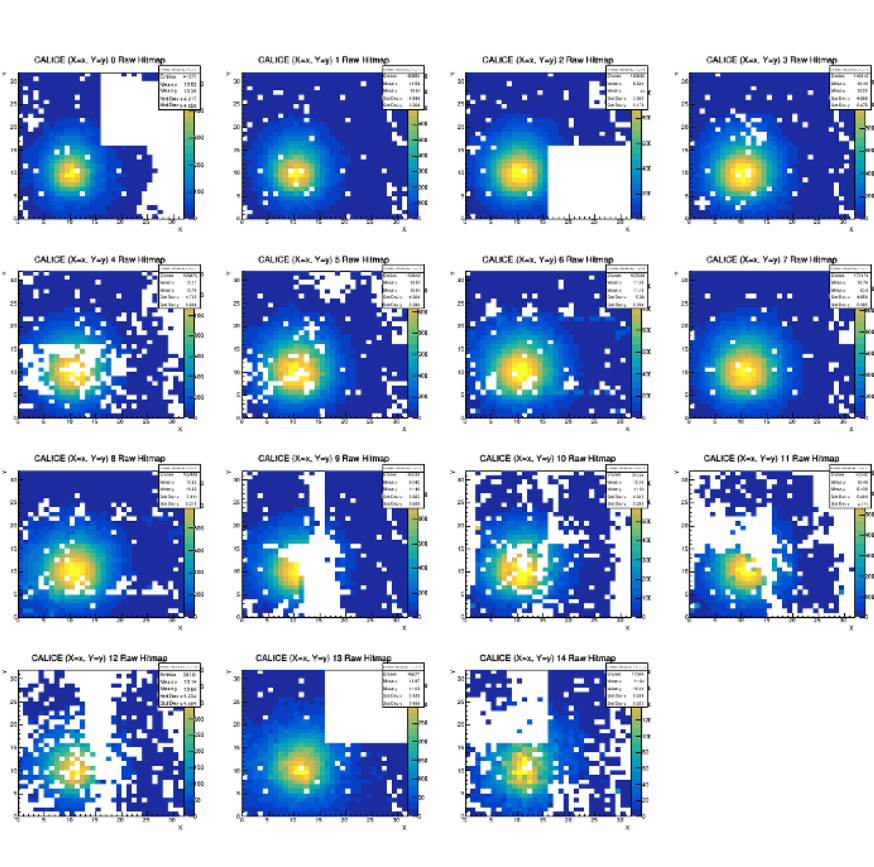
\includegraphics[keepaspectratio, scale=0.2]{Figure/Beamtest/hitmap_e20.png}
    \subcaption{$\SI{20}{GeV}$電子ビーム}
  \end{minipage}
    \begin{minipage}[b]{0.45\linewidth}
    \centering
    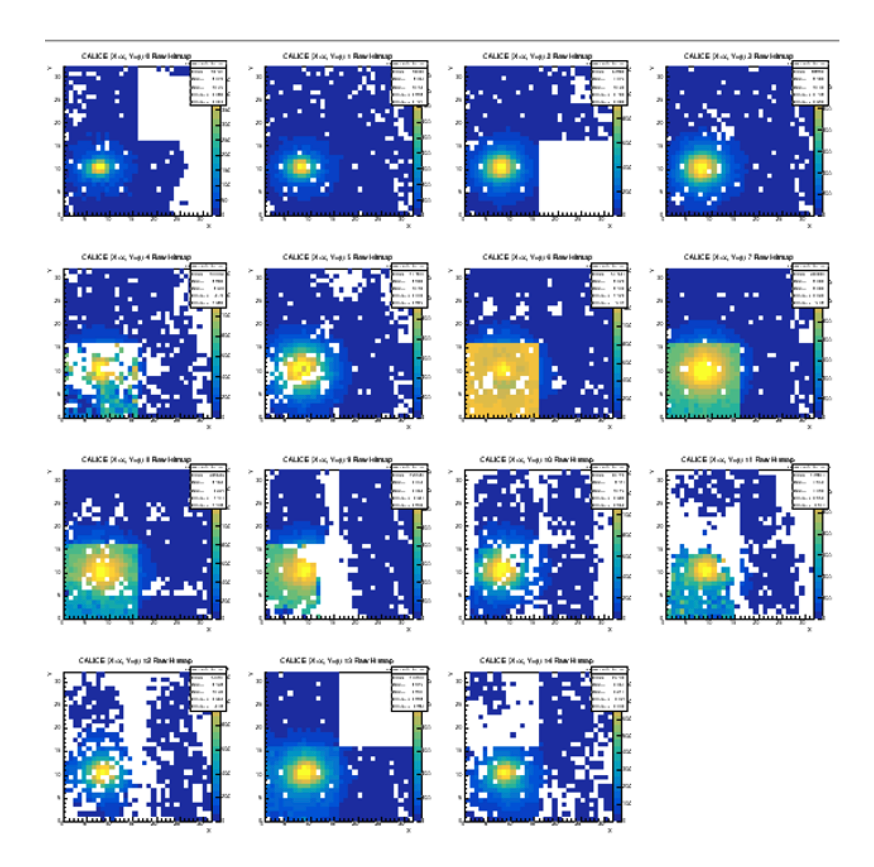
\includegraphics[keepaspectratio, scale=0.2]{Figure/Beamtest/hitmap_e150.png}
    \subcaption{$\SI{150}{GeV}$電子ビーム}
  \end{minipage}
  \begin{minipage}[b]{0.45\linewidth}
    \centering
    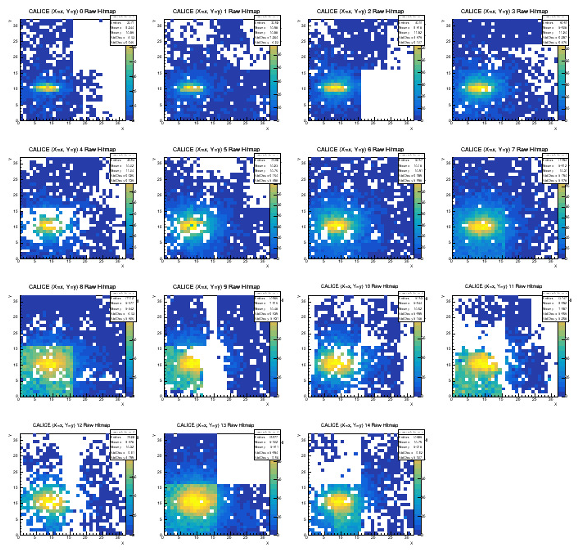
\includegraphics[keepaspectratio, scale=0.2]{Figure/Beamtest/hitmap_mu150.png}
    \subcaption{$\SI{150}{GeV}$ミューオンビーム}
   \end{minipage}
   \hfill
  \begin{minipage}[b]{0.45\linewidth}
    \centering
    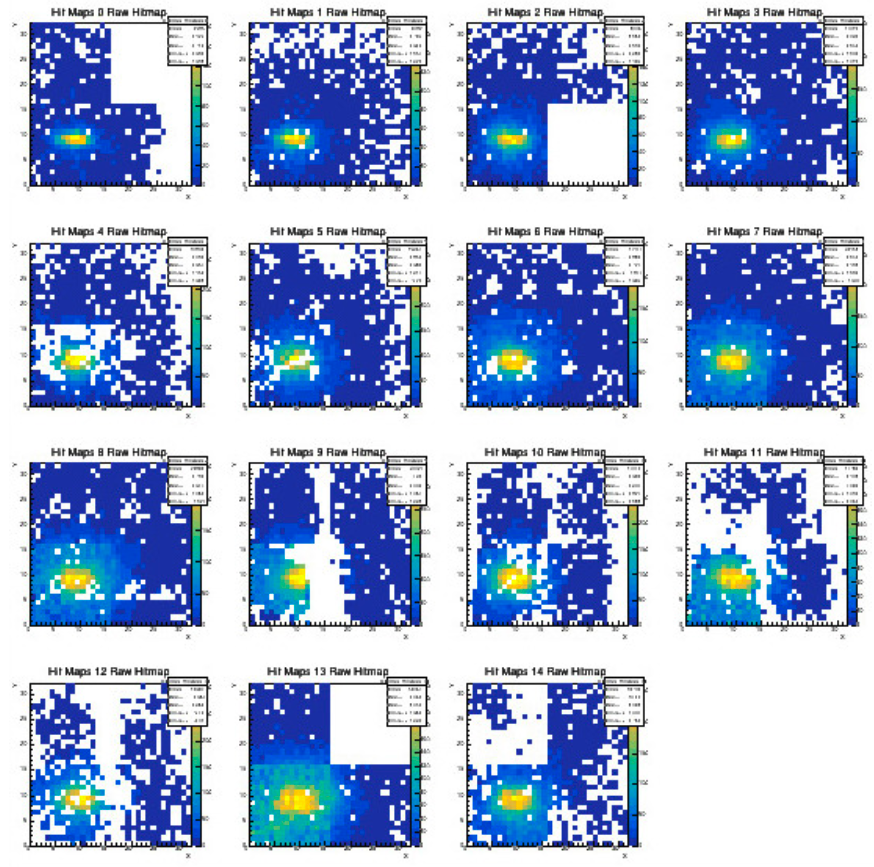
\includegraphics[keepaspectratio, scale=0.2]{Figure/Beamtest/hitmap_pi150.png}
    \subcaption{$\SI{150}{GeV}$パイ中間子ビーム}
  \end{minipage}
  \caption{各ビーム種類におけるヒットマップ。左上から0層右上が3層、右下が14層と順に並んでいる。}
  \label{hitmap}
\end{figure}
\subsection{ペデスタル}
続いて、ペデスタルの解析を行った。ペデスタルとはトリガーが入っていない時の信号の大きさで、エレクトロニクス由来のノイズ等によってその値の幅は変化する。実際のヒットによる信号の大きさは、得られたすべての値からペデスタルの値を引いた値になるため、ペデスタルについて十分に解析を行うことは重要となる。一般的にぺデスタルはガウス関数でフィッティングすることができ、その中央値はペデスタル信号の大きさを、標準偏差はその揺らぎの大きさ (ノイズ) に相当する。図\ref{pedestal}に各エネルギーの電子ビームのrunにおける同じチャンネルのペデスタルを示した。\\
\begin{figure}[H]
\begin{center}
 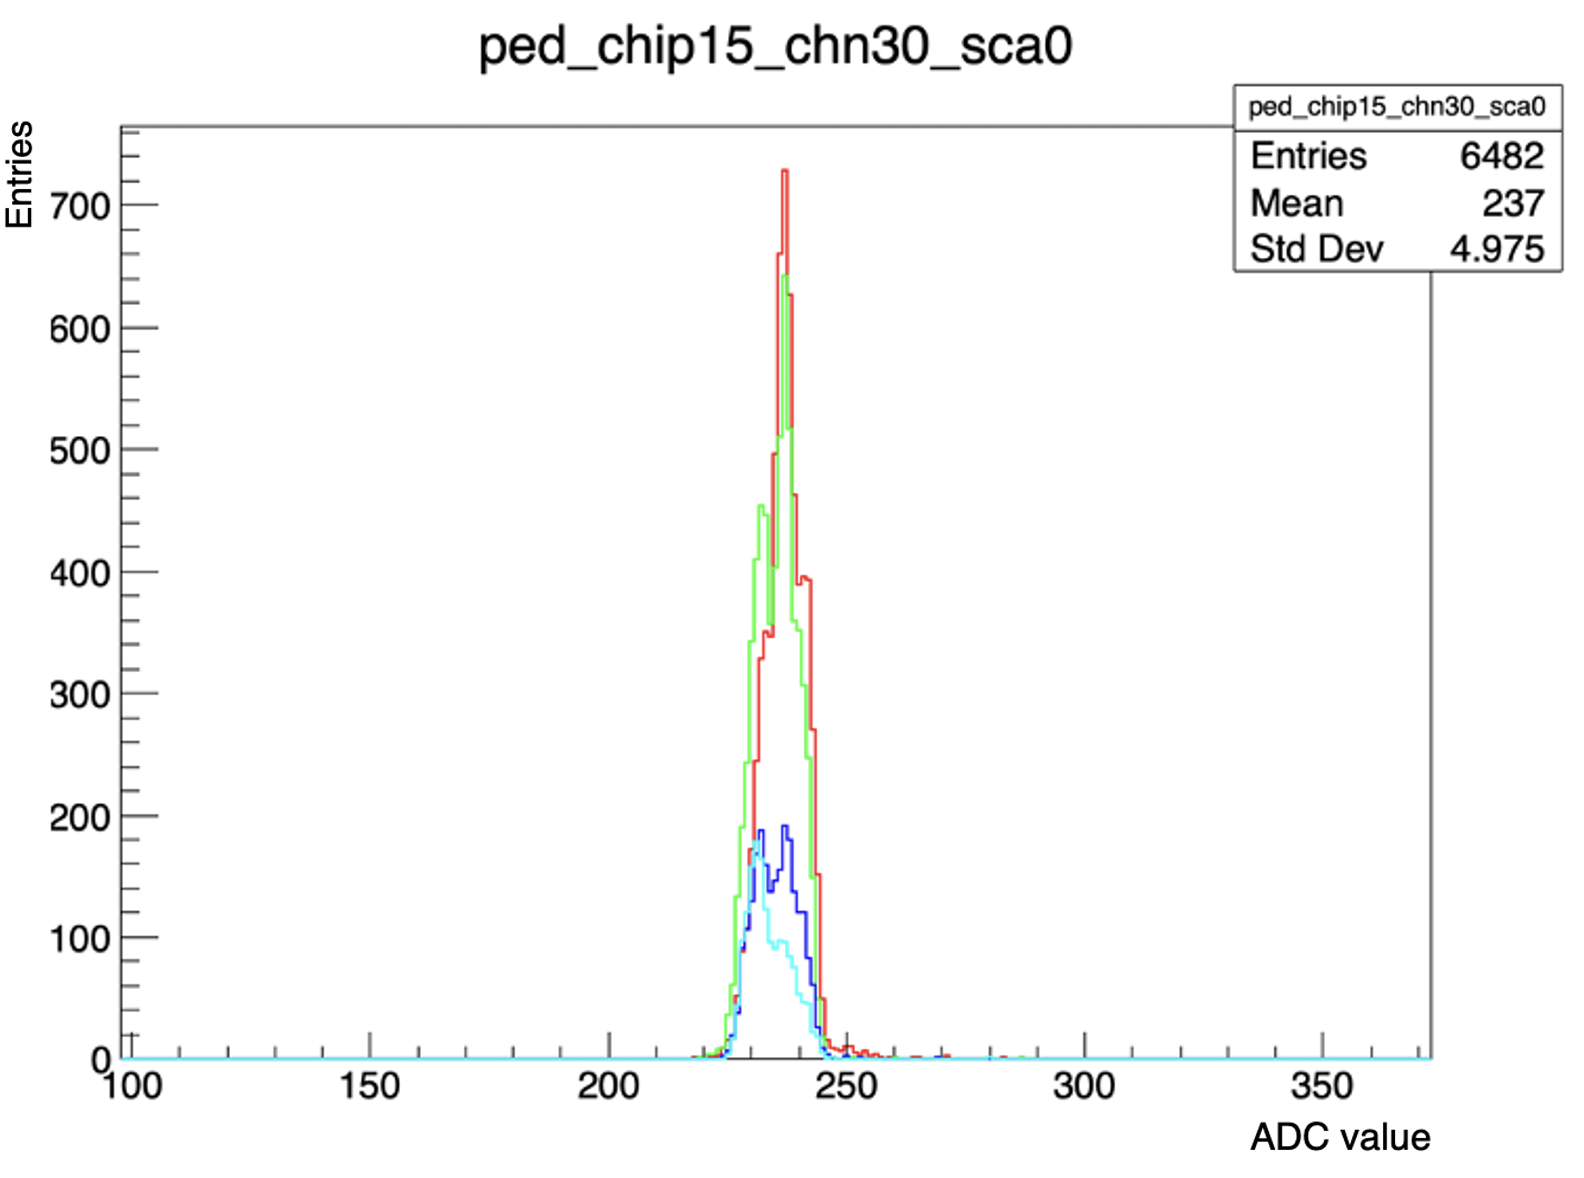
\includegraphics[keepaspectratio, scale=0.5]
 	{Figure/Beamtest/pedestal.png}
 		\caption{40/60/100/150$\mathrm{GeV}$の電子ビームにおけるペデスタル}
		\label{pedestal}
\end{center}
\end{figure}
\begin{figure}[H]
\begin{center}
 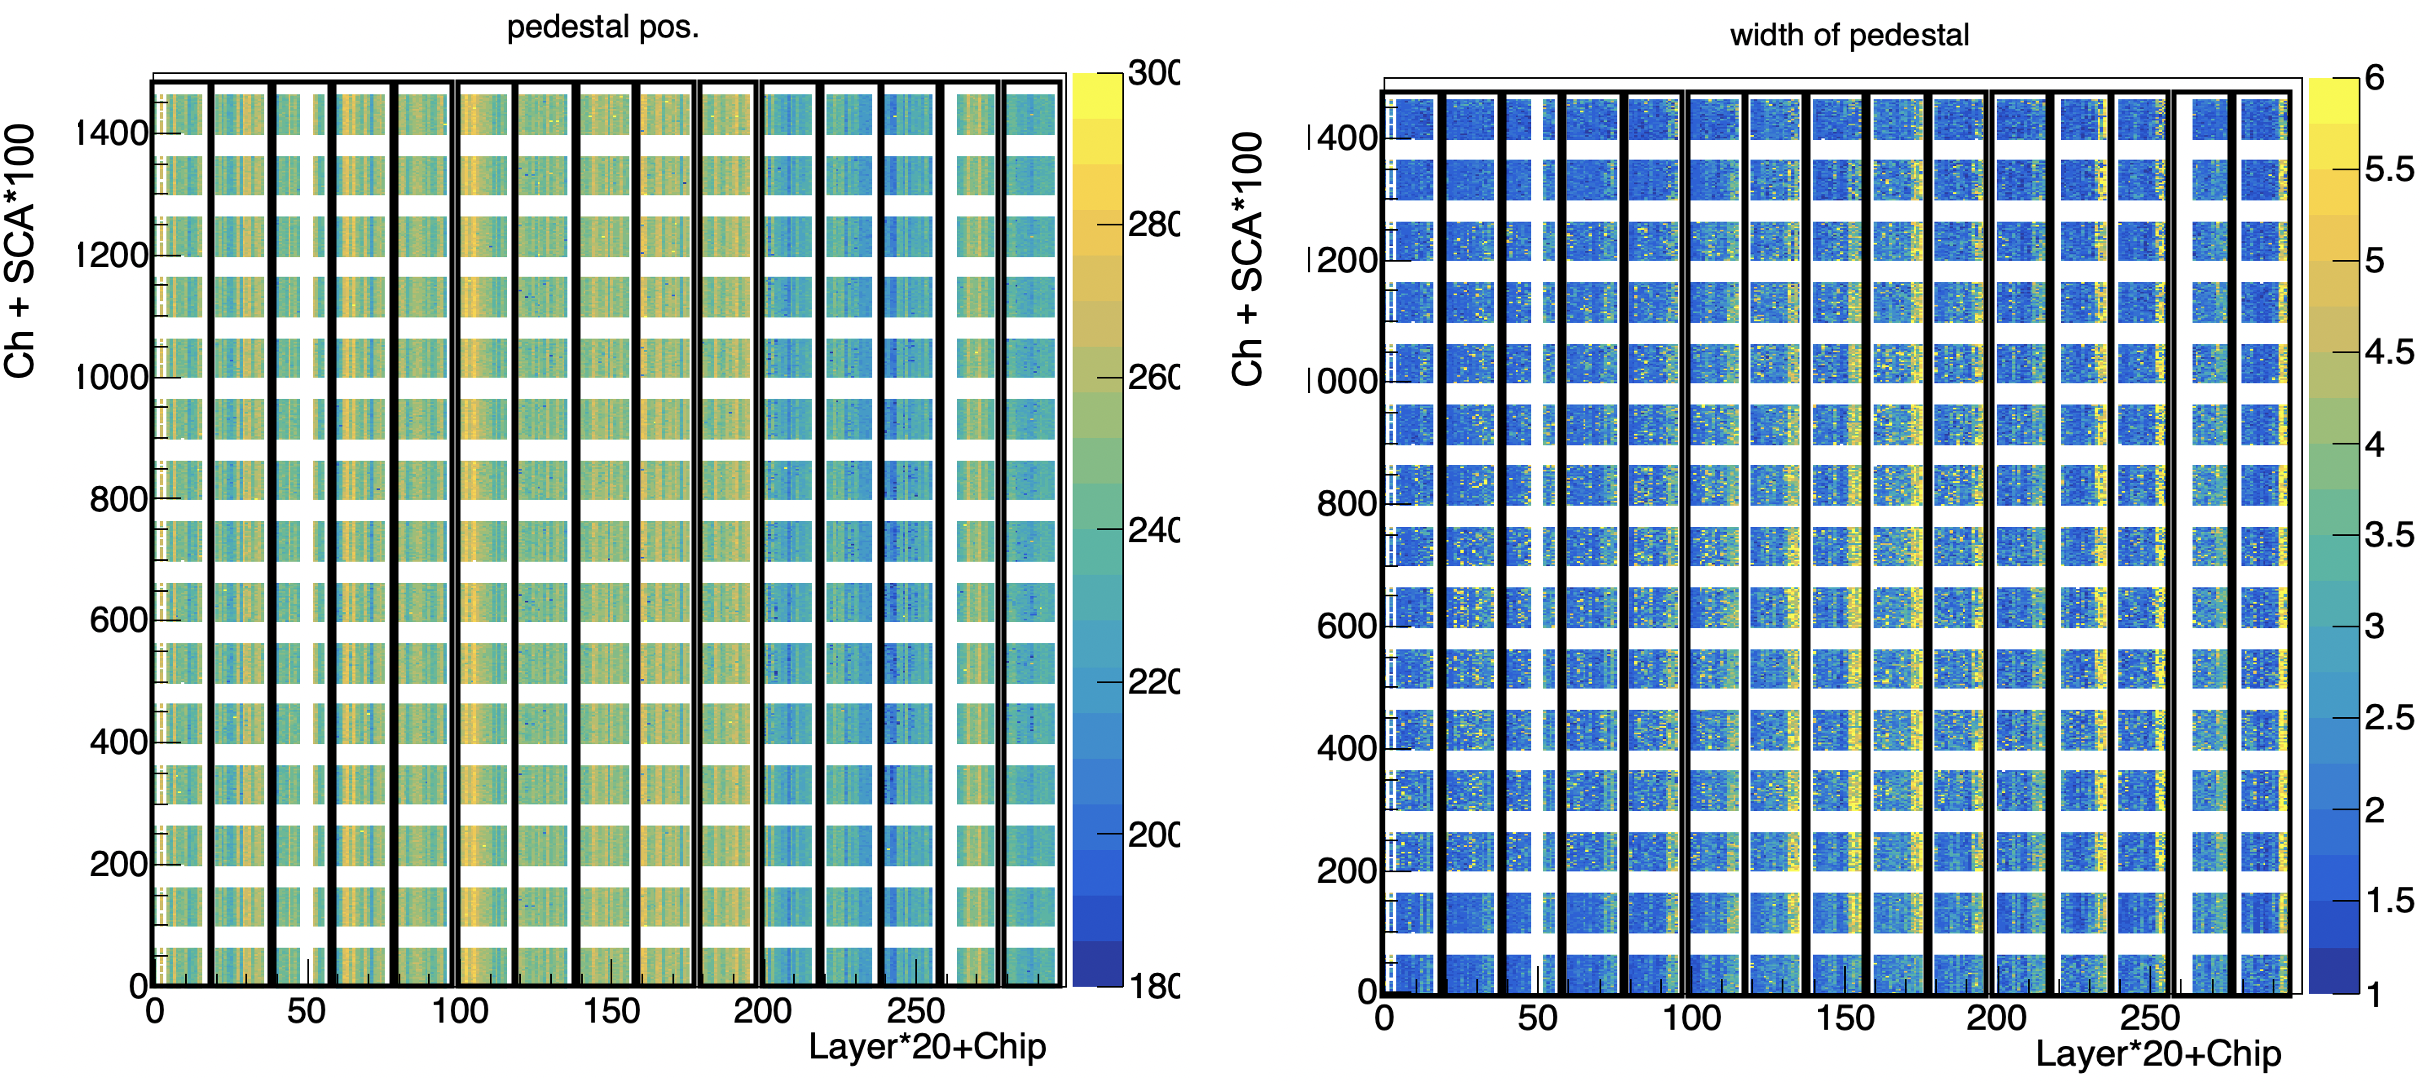
\includegraphics[keepaspectratio, scale=0.3]
 	{Figure/Beamtest/ped_pos.png}
 		\caption{ペデスタルをガウス関数フィットした際のパラメータ。横軸がチップを、縦軸がチャンネル番号を表しており、それぞれ全層、全SCAでの可視化のため、層数やSCAをかけた値となっている。(左) ガウス関数の中央値 (右) ガウス関数の幅の大きさ}
		\label{monitor}
\end{center}
\end{figure}

また、チャンネルによって図\ref{dp}に示すような2つのピークを持つペデスタルが確認された。このペデスタルピークが2つ見える現象をダブルぺデスタルと呼んで調査を行なった。
\begin{figure}[H]
\begin{center}
 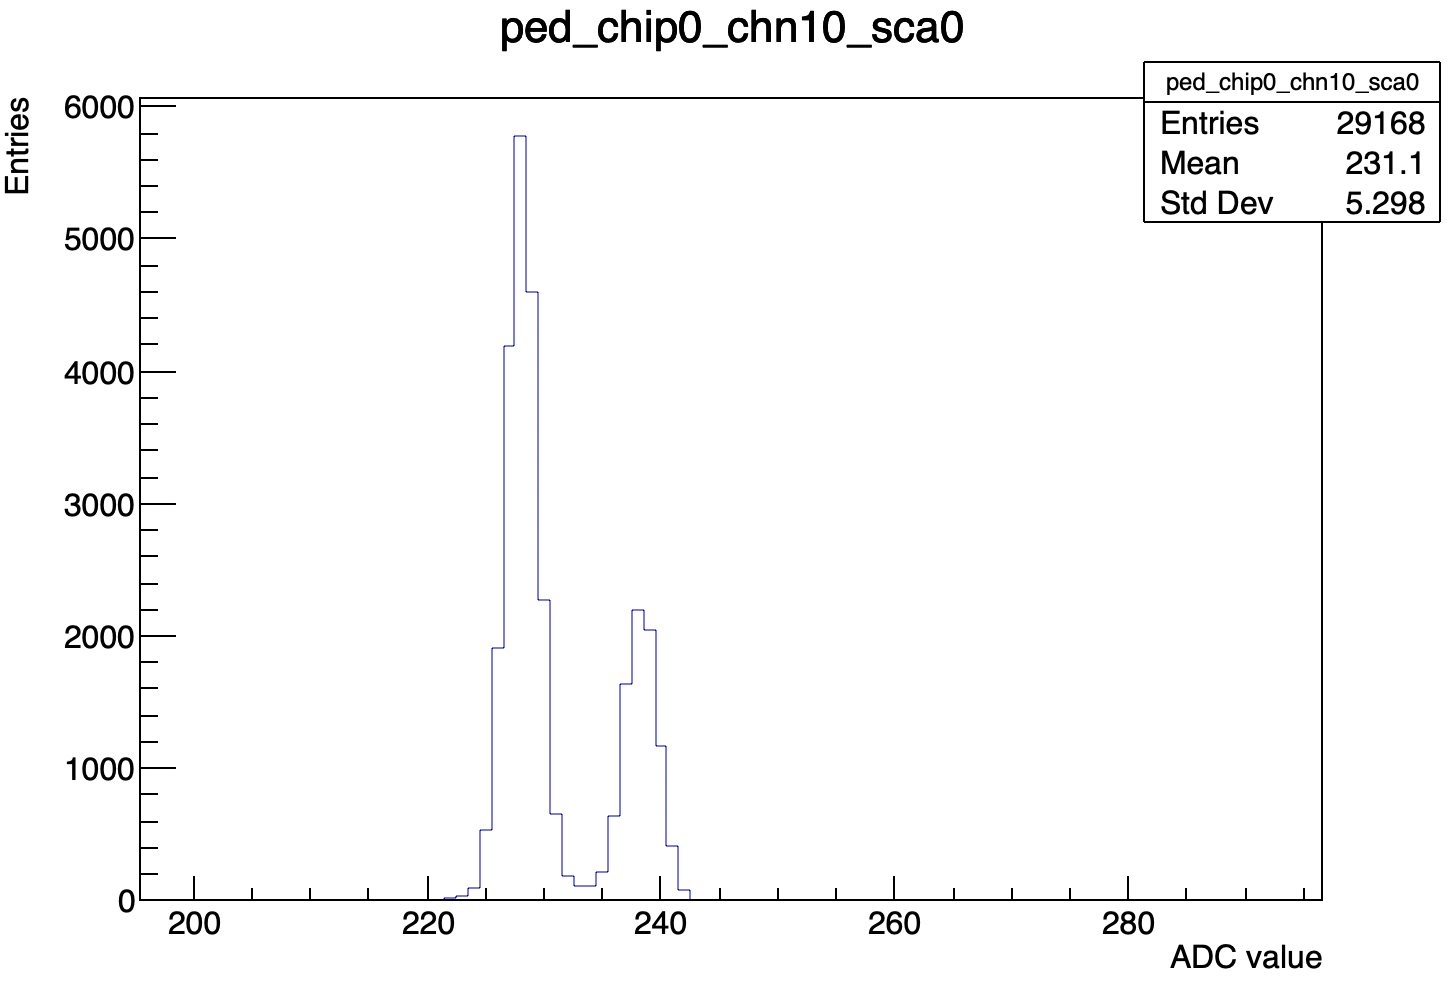
\includegraphics[keepaspectratio, scale=0.5]
 	{Figure/Beamtest/dp.png}
 		\caption{ダブルペデスタルの例}
		\label{dp}
\end{center}
\end{figure}
%\subsection{スクエアイベント}
\section{まとめと考察}
記入予定
(メモ:各Slabは実験前にモジュールへのインストールと動作確認を行い、緩衝材で梱包して輸送した。)
 % !TEX root = ../MasterThesis_Onoe.tex
% 上記はただのコメントではなく親ファイルの場所を教えているので
% 消してしまうとファイルごとのタイプセットができなくなるので注意。
% 親ファイル名を変更したときはここも変更する。

\chapter{深層学習} \label{sec:Deeplearning}
本章では、本研究で提案する手法である深層学習の理論を述べる。初めに、深層学習の基礎技術であるパーセプトロンについて説明する。そしてパーセプトロンを多層にしたニューラルネットの構造と計算技術について説明する。最後に深層学習のネットワークについて、特にグラフ構造のデータを扱うグラフニューラルネットワークについて紹介する。
\section{ニューラルネットワーク}
\subsection{パーセプトロン(単層ニューラルネットワーク)}
ニューラルネットワークの基礎となるパーセプトロンは、ローゼンブラットにより1957年に考案された。パーセプトロンの基本構造は、信号を入力として受け取り論理回路を通して出力信号を出すものである。図\ref{perceptron}に最も基本的なパーセプトロンの例を示す。\cite{dnnbook}\\
\begin{figure}[H]
	\begin{center}
 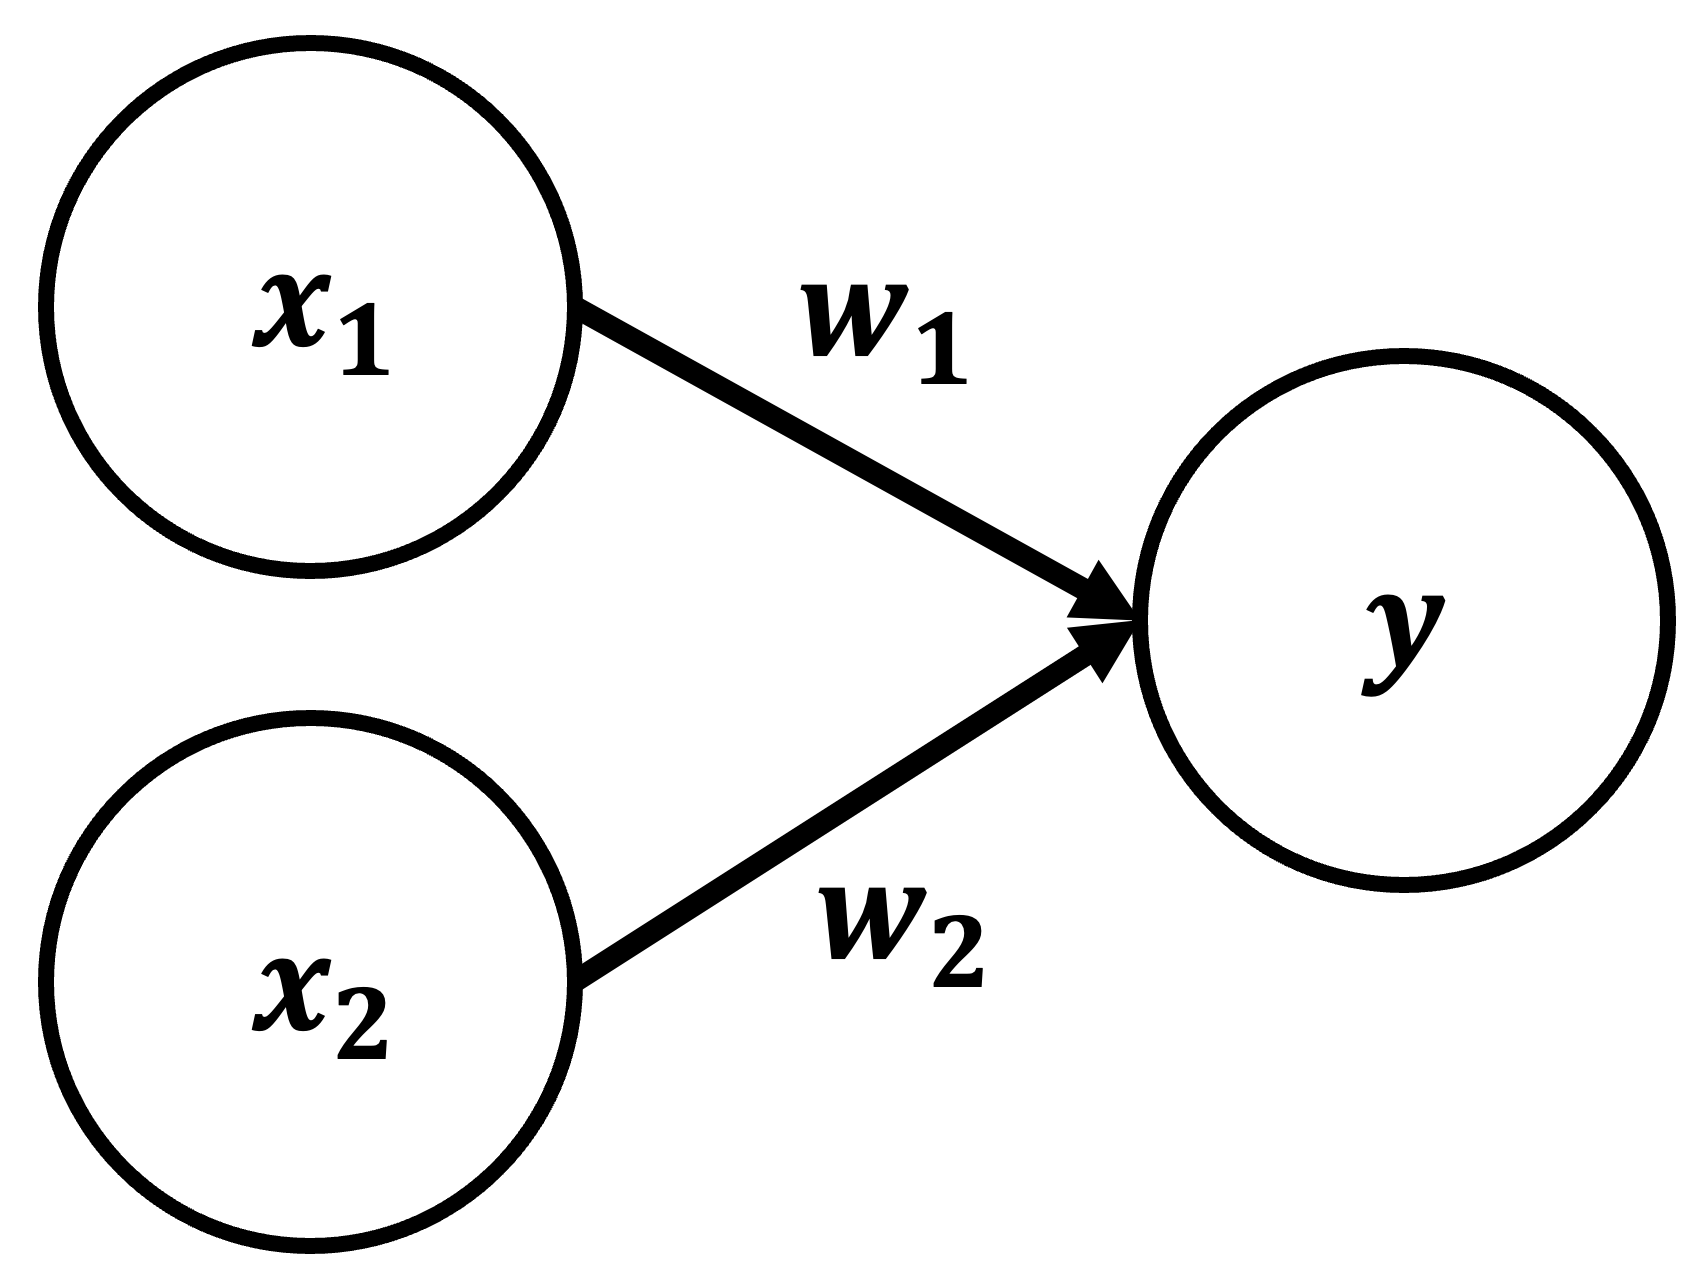
\includegraphics[keepaspectratio, scale=0.15]
 	{Figure/Deeplearning/perceptron.png}
 		\caption{パーセプトロン}
 		\label{perceptron}
	\end{center}
\end{figure}
$x_1, x_2$は入力信号、$y$が出力信号であり、$w_1,w_2$がそれぞれの入力信号にかかる重みを表す。また、図中における$\bigcirc$はノードと呼ぶ。入力信号はノードに送られる前に重みが掛けられ、出力ノードにてそれらの総和をとる。出力ノードでの演算(活性化関数)をステップ関数(階段関数)とすると、その総和が閾値$\theta$を超えている場合のみ出力信号は1を出力することになる。数式で示すと以下のようになる。\\
\begin{align}
 y =
 \begin{cases}
 0 & (w_1x_1 + w_2x_2 ) \leq \theta\\
 1 & (w_1x_1 + w_2x_2 ) > \theta \\
 \end{cases}
\end{align}
 パーセプトロンにおいて重要となるのは入力信号に対する固有の重みであり、重みは各信号の重要性を操作する要素として働く。すなわち重みが大きいほど、対応する信号の全体における重要性が高くなる。この重みを更新する操作を学習と呼び、ニューラルネットワークでは学習を繰り返すことで重みパラメータを理想とする値に近づけていく。\\
 また、入力信号が3つ以上の場合についても考えることができ、以下のような式で表される。入力信号$x = \{ x_1, x_2, \ldots x_n \}$、重みパラメータ$w = \{ w_1, w_2, \ldots w_n \}$、活性化関数(ここではステップ関数)を$h(x)$とすると、出力ベクトルyは以下のようになる。
\begin{align}
y = h(w^T x) =
 \begin{cases}
 0 & (w_1x_1 + w_2x_2 + \ldots + w_nx_n) \leq \theta\\
 1 & (w_1x_1 + w_2x_2 + \ldots + w_nx_n) > \theta \\
 \end{cases}
\end{align}
\subsection{多層パーセプトロン(多層ニューラルネットワーク)}
パーセプトロンの演算では線形領域のみしか表現できず、非線形領域においても扱えるよう入力層と出力層の間に中間層(隠れ層)を加えるニューラルネットワークに改良された。このような中間層を複数重ねたパーセプトロンを多層パーセプトロン(Multi Layer Perceptron, MLP)と呼ぶ。多層パーセプトロンの簡単な例を図\ref{mlp}に示す。\\
\begin{figure}[H]
	\begin{center}
 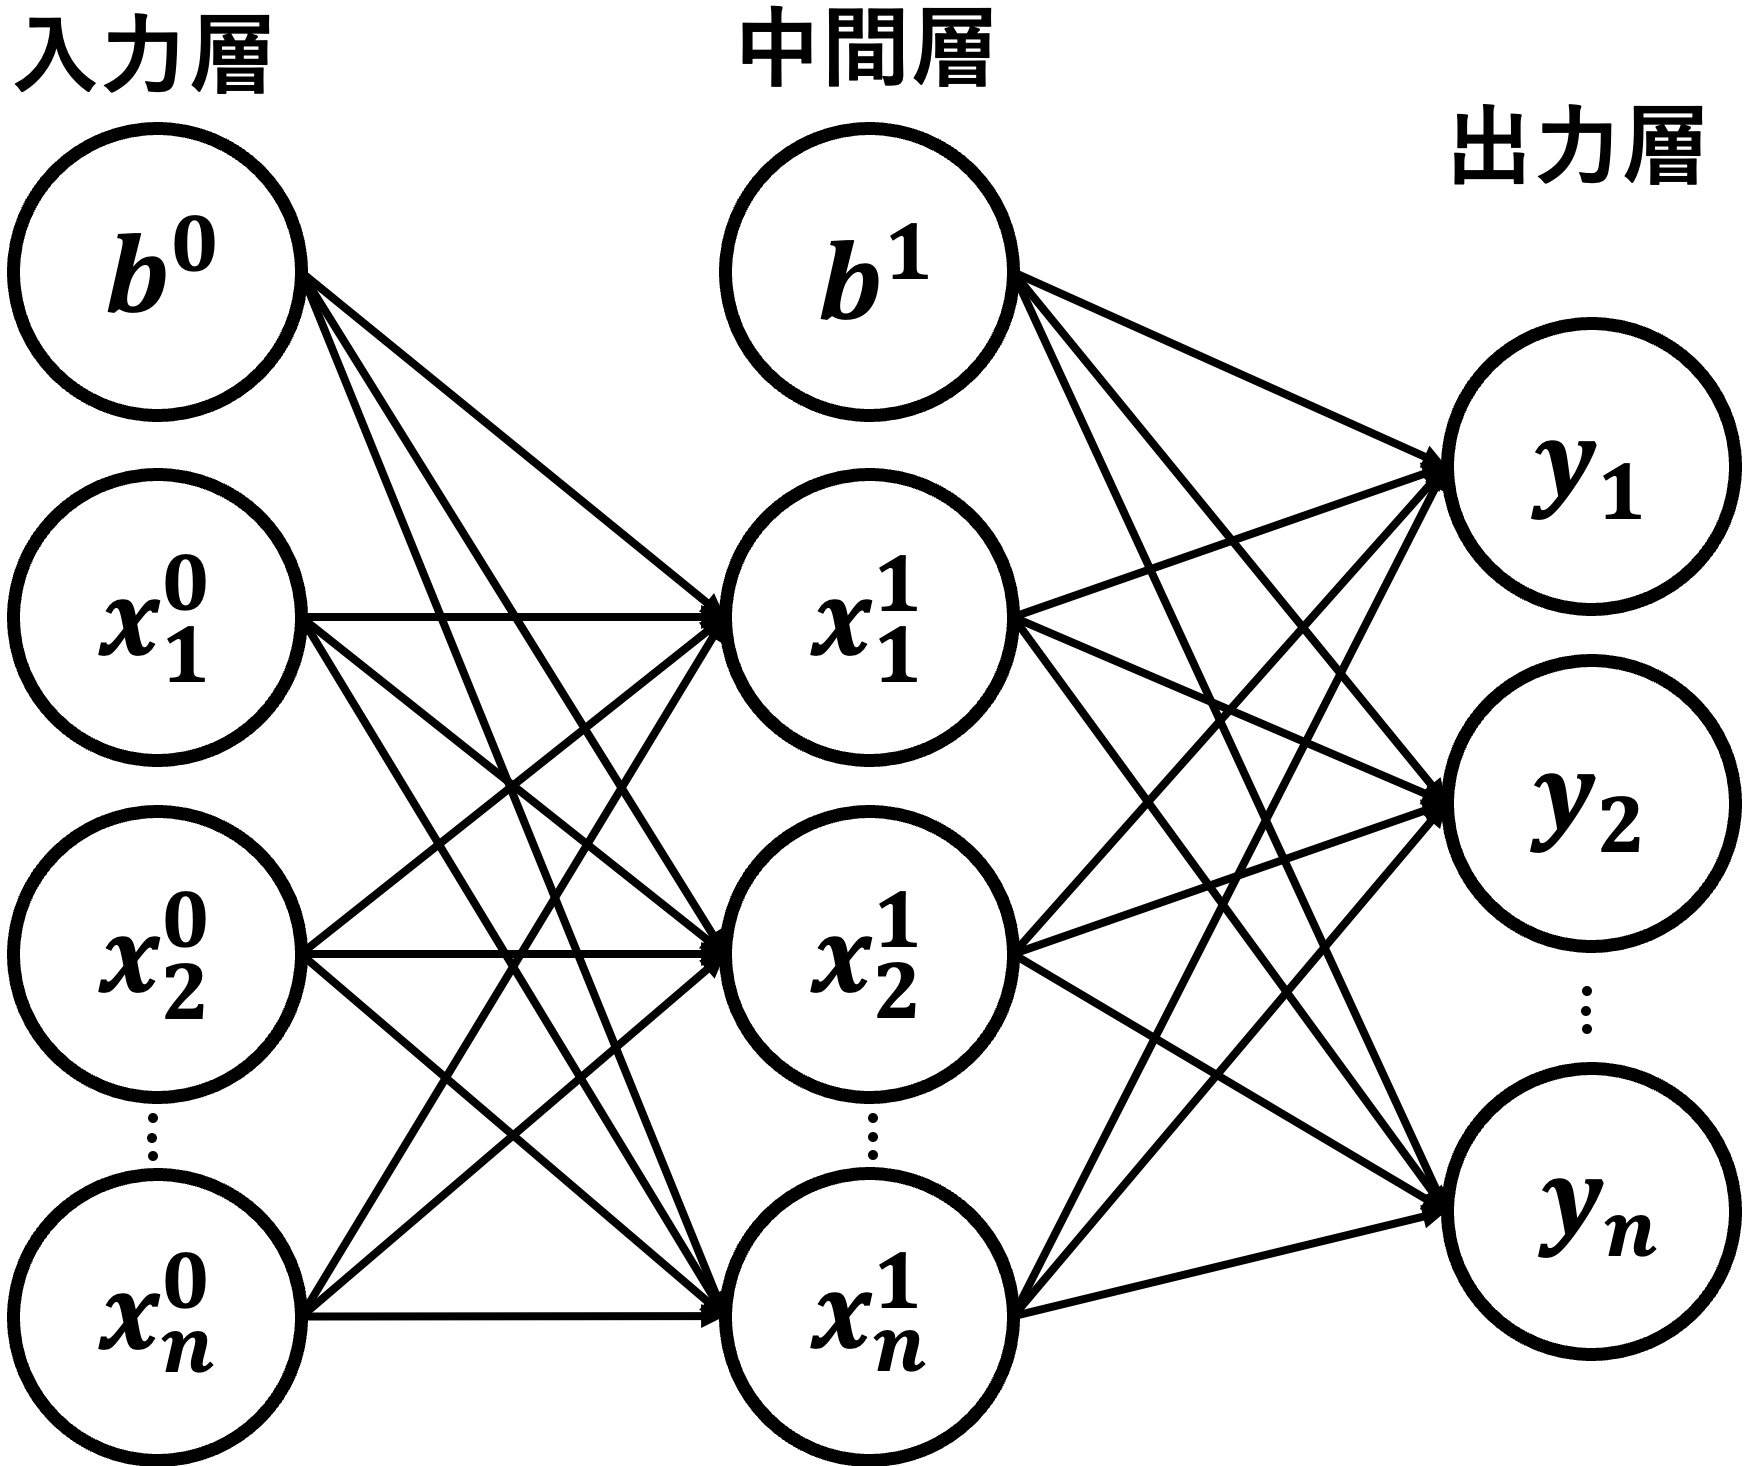
\includegraphics[keepaspectratio, scale=0.2]
 	{Figure/Deeplearning/mlp.png}
 		\caption{多層パーセプトロン(ニューラルネットワーク)}
 		\label{mlp}
	\end{center}
\end{figure}
最も左のノード列を入力層、真ん中のノード列を中間層、一番右のノード列を出力層とすると、以下のような数式で表される。入力信号$x^0 = \{ x_1^0, x_2^0, \ldots x_n^0 \}$、中間層の各ノードに入ってくる信号$x^1 = \{ x_1^1, x_2^1, \ldots x_n^1 \}$、入力層と中間層の信号にかかる重みパラメータがそれぞれ$w^0 = \{ w_1^0, w_2^0, \ldots w_n^0 \}, w^1 = \{ w_1^1, w_2^1, \ldots w_n^1 \}$、活性化関数を$h(x)$とすると、出力ベクトル$y_n$は
\begin{align}
x_1^1 = h(w_1^0 x_1^0 + w_2^0 x_2^0 + w_3^0 x_3^0 + \cdots + w_n^0 x_n^0 + b^0)\\
y_n = h(w_1^1 x_1^1 + w_2^1 x_2^1 + w_3^1 x_3^1 + \cdots + w_n^1 x_n^1 + b^1)
\end{align}
となる。ここで、$b^n$としてより学習にパラメータを加えるため、各層に実数値のバイアスを導入した。重みと信号の積の和を$a$として、上式に行列を用いると簡略に表現できる。\\
\begin{align}
\mathbf{y} = h(\mathbf{a})\\
\mathbf{a} = \mathbf{W} \mathbf{x} + \mathbf{b}
\end{align}
 以下ではニューラルネットワークの学習における、学習の仕組みや重要な技術について取り上げる。
\subsubsection{活性化関数}
活性化関数はニューラルネットワークにおける入力の重み線形和から、出力を決定するための関数である。活性化関数には、非線形演算によって表現力を高めるために非線形関数が用いられることが多く、以下に主なものについて示す。中でもReLU関数は、勾配の最大値が1であることから勾配消失を起こしにくく、計算の安定性の理由から多くのモデルにおいて用いられている。(sigmoid関数の場合$x=0$でピークを持ち、それ以外で急速に小さくなってしまう)
\begin{itemize}
	\item ステップ(階段)関数
		\begin{align}
			h(a) =
			\begin{cases}
			0 & (a \leq \theta)\\
			1 & (a > \theta)
			\end{cases}
		\end{align}
	\item sigmoid関数
		\begin{equation}
			h(a) = \frac{1}{1+\exp(-a)}
		\end{equation}
	\item $\tanh$関数
		\begin{equation}
			h(a) = \tanh(a)
	\end{equation}
	\item ReLU関数(ランプ関数)
		\begin{align}
			h(a) =
			\begin{cases}
			0 & (a \leq \theta)\\
			a & (a > \theta)
			\end{cases}
		\end{align}
	\item LeakyReLU関数 (s=0.01が多い)
		\begin{align}
			h(a) =
			\begin{cases}
			sa & (a \leq \theta)\\
			a & (a > \theta)
			\end{cases}
		\end{align}
\end{itemize}
\begin{figure}[H]
  \begin{minipage}[b]{0.45\linewidth}
    \centering
    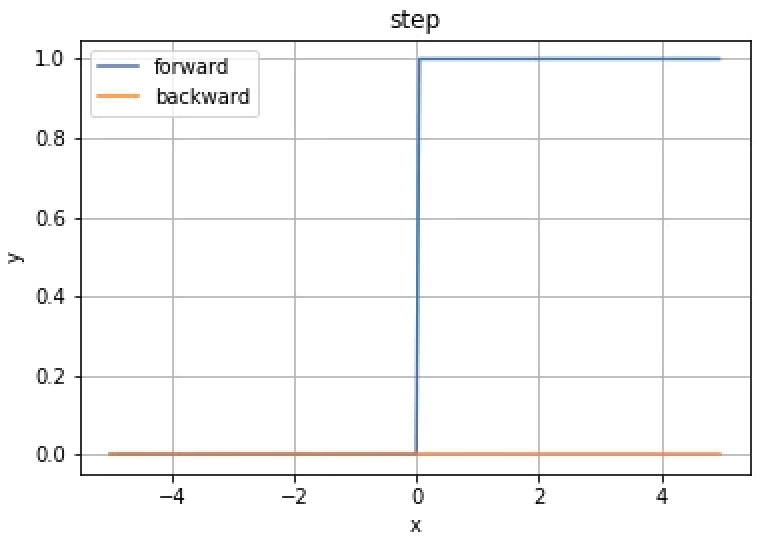
\includegraphics[keepaspectratio, scale=0.25]{Figure/Deeplearning/step.png}
    \subcaption{ステップ関数}
  \end{minipage}
    \begin{minipage}[b]{0.45\linewidth}
    \centering
    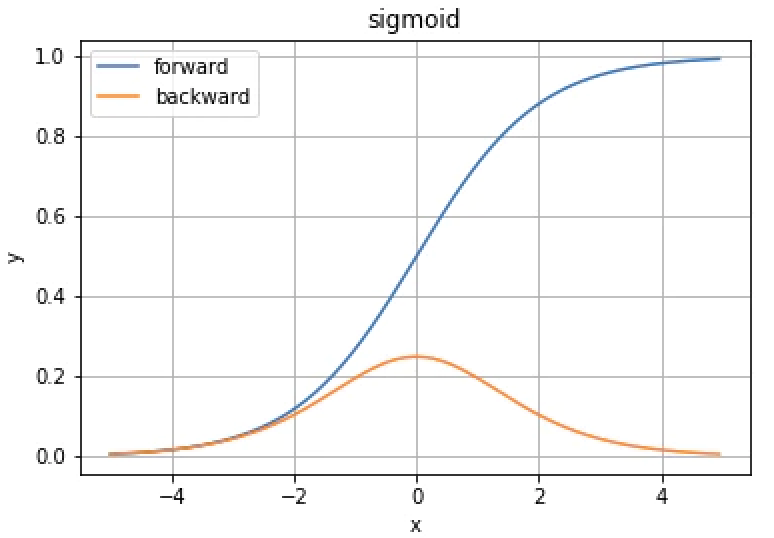
\includegraphics[keepaspectratio, scale=0.25]{Figure/Deeplearning/sigmoid.png}
    \subcaption{sigmoid関数}
  \end{minipage}
  \begin{minipage}[b]{0.45\linewidth}
    \centering
    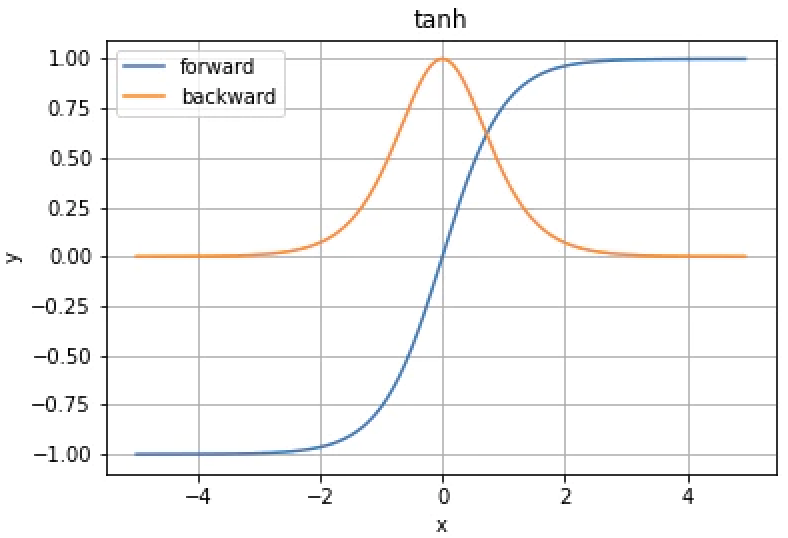
\includegraphics[keepaspectratio, scale=0.25]{Figure/Deeplearning/tanh.png}
    \subcaption{$tanh$関数}
   \end{minipage}
  \begin{minipage}[b]{0.45\linewidth}
    \centering
    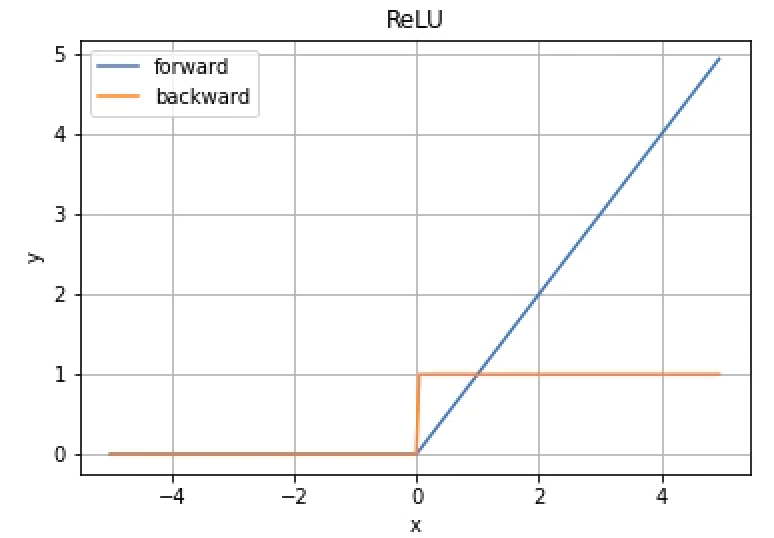
\includegraphics[keepaspectratio, scale=0.25]{Figure/Deeplearning/ReLU.png}
    \subcaption{ReLU関数}
  \end{minipage}
  \begin{minipage}[b]{0.45\linewidth}
    \centering
    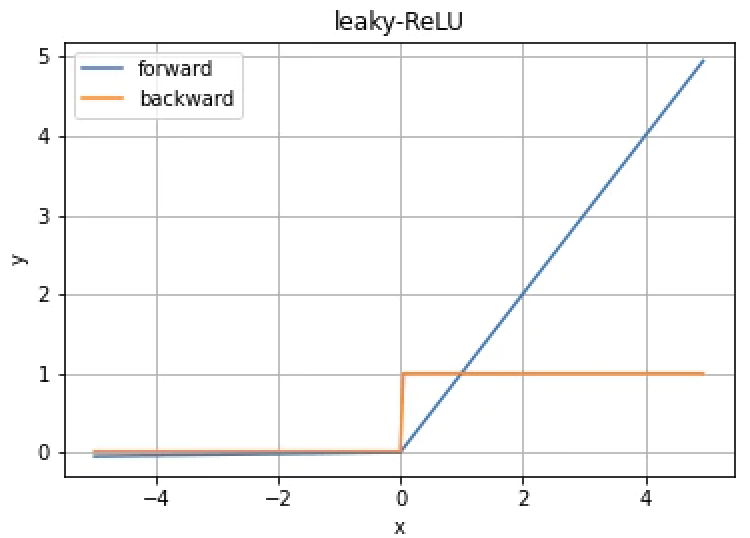
\includegraphics[keepaspectratio, scale=0.25]{Figure/Deeplearning/LeakyReLU.png}
    \subcaption{LeakyReLU関数}
  \end{minipage}
  \caption{活性化関数のグラフ。Forwardは順方向、backwardは逆方向 (後に誤差逆伝播法で説明) の際の演算を表す。}
  \label{hitmap}
\end{figure}
\subsubsection{出力層の設計}
ニューラルネットワークで扱える問題は、主に回帰問題と分類問題に分けられる。それぞれの問題によって出力層の設計が異なり、回帰問題においては恒等関数が、分類問題においてはソフトマックス関数が用いられる。恒等関数では入力された値をそのまま出力する。ソフトマックス関数は以下の式\ref{softmax}のように、0から1までの値を出力する関数であり、それぞれのカテゴリに分類される確率を表す。ここで$y_k$はニューラルネットワークの出力、$x_k$は出力層へ入ってくる信号を表す。また、出力層のノード数は問題に合わせて適宜調整する必要があり、分類問題であればカテゴリ数だけノードを設計する必要がある。
\begin{align}
\label{softmax}
y_k = \frac{\exp(x_k)}{\sum_{i=1}^n \exp(x_i)}
\end{align}

\subsubsection{損失関数}
先述の通り、ニューラルネットワークでは学習によって重みを更新するが、その際に学習結果を正しい答えと照らし合わせて評価し、その評価値を最小にするように重みを更新する。この評価関数を損失関数 (Loss function) と呼ぶ。損失関数には主に以下の2つが用いられる。
\begin{itemize}
	\item 二乗和誤差関数  (Mean Squared Error) \\
		二乗和誤差関数は、以下の式\ref{mse}で定義される関数である。ここで、$y_k$はニューラルネットワークの出力、$t_k$は正解ラベルを表し、kはデータの次元数を表す。二乗和誤差関数の微分値はyの一次関数となっていることから、出力・正解ラベルが共に連続値であり恒等関数を出力層に持つ回帰問題で採用される。
		\begin{align}
			\label{mse}
			L = \frac{1}{2}\sum_k {(y_k-t_k)}^2
		\end{align}
	\item 交差エントロピー誤差 (Cross Entropy Error) 
		交差エントロピー誤差は、以下の式\ref{cee}で定義される関数である。ここで、$y_k$はニューラルネットワークの出力で、$t_k$はone-hot表現の正解ラベルを表す。交差エントロピー誤差は主にソフトマックス関数を出力層に用いる分類問題において採用される。
		\begin{align}
			\label{cee}
			L = - \sum_k t_k \log(y_k)
		\end{align}
\end{itemize}

\subsubsection{誤差逆伝播法}
これまではニューラルネットワークの順方向の伝播(forward propagation)について見てきたが、出力層において学習結果と正解ラベルを比較し、逆方向に信号を伝播させ重みを更新するアルゴリズムを誤差逆伝播法 (back propagation) という。誤差逆伝播法では、次のような処理を行う。
\begin{enumerate}
	\item ニューラルネットワークにおいて順方向に学習を行い、出力層で損失関数によって正解ラベルとの誤差を求める。
	\item 誤差から各出力層ノードについて期待される出力と重要度、誤差を計算する。(局所誤差)
	\item 特に重要度の高い前層の入力が、局所誤差に影響を及ぼしているとして重みを調整する。
	\item 合成関数の微分によって、さらに前層へと処理を繰り返す。
\end{enumerate}
これによって重みを修正していく学習が可能になっており、また勾配の計算には活性化関数の偏微分が積をとって含まれているため、ネットワークの演算は全体を通して微分可能となっている。
\subsubsection{前処理}
ニューラルネットワークでは、前処理を行うことで識別性能の向上や学習の高速化を見込むことができる。前処理の手法には以下にあげるようなものがあり、データ全体の分布を考慮して適応する必要がある。
\begin{itemize}
 \item 正規化:最小値を0、最大値を1とするスケーリング
 \begin{align}x'_i = \frac{(x_i - min(x))}{max(x)-min(x)}\end{align}
 \item 標準化:平均を0、分散を1とするスケーリング
 \begin{align}x'_i = \frac{(x_i - \bar{x})}{\sigma}\end{align}
 \item 対数変換:外れ値による分散を小さくし、0付近の値を区別しやすくする。
 \begin{align}x'_i = \ln(x_i)\end{align}
\end{itemize}
\subsubsection{ミニバッチ処理}
ニューラルネットワークを学習させるにあたって、データを1つ1つ学習させるわけではない。実際にはミニバッチと呼ばれる、学習データをいくつかまとめて束としたものを一度に学習させる。この束をミニバッチという。また、このミニバッチのサイズ、つまりいくつのデータをまとめて束にするかという値のことをバッチサイズという。数値計算を扱うライブラリの多くは、大きな配列の計算を効率よく処理できるよう最適化がなされており、ミニバッチによる学習を行うことで、処理時間を短縮することができる。一方で、ミニバッチのデータは誤差逆伝播においてバッチ内で損失関数の和を用いているため、バッチサイズによって学習結果が異なり、サイズが大きい場合には学習精度が悪くなってしまう可能性もある。
\subsubsection{最適化アルゴリズム}
ニューラルネットワークの学習では、損失関数の値が最小となるような最適なパラメータを探索する。しかし損失関数のパラメータ空間は非常に複雑であることから、最適化は難しい。以下では、勾配降下法をはじめとする最適化手法について述べる。また、一度の学習で更新するパラメータの度合いを学習率 (learning rate) と呼んでおり、ネットワークの重みなどのパラメータとは異なり、学習率のような人の手で設定する必要のあるパラメータをハイパーパラメータと呼ぶ。
\begin{itemize}
\item \textbf{勾配降下法}\\
現在のネットワークのパラメータの微分 (勾配) を計算し、その微分の値を手がかりにパラメータの値を徐々に更新する方法を、勾配降下法 (gradient descent method) という。勾配降下法は以下の式\ref{gd}のように表される。ここで、$\mathbf{W}$は更新する重みパラメータを、$L$は損失関数を、$\eta$は学習率を表す。
\begin{align}
 \label{gd}
 \mathbf{W} \leftarrow \mathbf{W} - \eta \frac{\partial L}{\partial \mathbf{W}}
\end{align}
 また、ミニバッチ学習を用いた勾配降下法は特に、確率的勾配降下法 (stocastic gradient descent, SGD) と呼ばれており、現在のニューラルネットワークの最適化法は主にSGDに基づいて設計されている。しかし、SDGには関数の形状が等方的でない場合、勾配の方向が最終的な最小値と異なるため探索が非効率になるという欠点があり、単純に勾配方向へ進む以外の方法としてさまざまな最適化手法が考案されている。
\item \textbf{モーメンタム}\\
モーメンタム (Momentum) は、それまでの学習における損失関数上で更新ステップの動きを考慮することでSGDの振動を抑えるアルゴリズムである。モーメンタムにおける更新方法は、物理学の速度にあたる変数$\mathbf{v}$を加え、以下の式のように表される。
\begin{align}
\mathbf{v} \leftarrow \alpha \mathbf{v} - \eta \frac{\partial L}{\partial \mathbf{W}}\\
\mathbf{W} \leftarrow \mathbf{W} + \mathbf{v}
\end{align}
上式における$\alpha \mathbf{v}$が、Uの字の斜傾を転がるボールが徐々に減速する運動のような役割を果たし、振動を抑えている。
\item \textbf{AdaGrad}\\
AdaGradでは、モーメンタムと同様にSGDの振動を抑えるが、学習率を減衰させることによってこれを達成するアルゴリズムである。AdaGradの更新方法は次のような式で表される。
\begin{align}
\mathbf{h} \leftarrow \mathbf{h} + \frac{\partial L}{\partial \mathbf{W}} \odot \frac{\partial L}{\partial \mathbf{W}} \\
\mathbf{W} \leftarrow \mathbf{W} - \eta \frac{1}{\sqrt{h}} \frac{\partial L}{\partial \mathbf{W}}
\end{align}
ここで、$\mathbf{h}$はこれまでの勾配の値を二乗和として保持する役割を持つ。そして$\eta \frac{1}{\sqrt{h}}$によって学習率のスケールを調整することができる。これによって動いた大きさに合わせてパラメータ毎に学習率の減衰を行うことができる。
\item \textbf{Adam}\\
Adamはモーメントの考えとAdaGradの考えを融合させた手法であり、モーメントの変数2つと前のステップまでの学習係数を表す変数1つの3つをハイパーパラメータにもつ。これによって効率的にパラメータ空間を探索することができる。
\item \textbf{RAdam}\\
RAdamはAdamにWarmupによる改良を行った最適化手法であり、これまで挙げた手法では、学習の初期段階ではサンプル数が少ないために、適応学習率の分散が極めて大きくなり粗悪な局所的最適解に陥ってしまうという課題があった。それに対して学習初段階の学習率を下げるWarmup手法によって、学習率の分散を自動的に抑えられるようなパラメータ空間を探索することができる。
\end{itemize}
\subsubsection{過学習}
深層学習には、ネットワークモデルが学習用データに過度に適合し過ぎてしまい、新しいデータに対する性能が低下してしまう、過学習 (Overfitting) という状態が発生する場合がある。これはデータがパラメータを大量に持ち、表現力が極めて高いモデルである場合や、学習用データの数が少ない場合に多く見られ、モデルがトレーニングデータに含まれるノイズ、または特異的な特徴に過度に適合するために起きてしまうものとされている。そのため、深層学習の実装においては過学習を防止するいくつかの方法を用いることが多く、以下に代表的なものを挙げる。
\begin{itemize}
\item ドロップアウト (Dropout)\\
ニューラルネットワークでは全てのノード同士が繋がっており演算を行っていたが、ニューロンをランダムに消去することで表現力が高すぎることによる過学習を抑制するというアプローチがあり、ドロップアウトという。これは機械学習におけるアンサンブル学習に近く、各epochの学習でそれぞれ違うモデルを学習させていると解釈することができる。
\item 荷重減衰 (Weight Decay)\\
適合しすぎる学習では、重みパラメータが極端に大きい値をとってしまっている場合が多く存在する。そのため重みに制限をかけることで重みが大きくなることを抑制する荷重減衰 (Weight Decay) という手法が存在する。具体例として、重みの二乗ノルム (L2) を損失関数$\mathrm{L}$に加算する場合には、以下のような制限がかかる。
\begin{align}
\mathrm{L} = E + \frac{1}{2}\lambda \sum_k {(w_k)}^2
\end{align}
ここで、Eは通常の誤差関数(損失関数)、$\lambda$は正則化の強さを表す正則化パラメータ、$w$が重みパラメータを表す。またL2正則化の他にも、重みの絶対値の和をとるL1正則化や絶対値最大の成分の絶対値に$\lambda$をかけるL$\infty$などが存在する。これらによって重みパラメータに強いペナルティが課せられた上で損失関数の値を最小にする学習を行うことができる。
\item 重み初期化\\
荷重減衰と同様に重みを大きくしないための手法として、重みの初期値を定める手法も存在する。重みは小さければ良いというものではなく、0の場合には誤差逆伝播法において全ての重みの値が同じように更新されてしまうため、正しくは重みを対称的な構造を持たないものにすることが重要となる。その手法にはランダムな重みを振る手法など様々なものがあり、中でもXavier Glorotによる手法が一般的に用いられる。この手法では、ニューラルネットにおいて入力層と出力層の重みが、ノード数を$n$とした時$\frac{1}{\sqrt{n}}$の標準偏差を持つガウシアンになるという初期化を行う。
\item 正規化 (Batch Normalization)\\
ミニバッチ毎の入力特徴量をスケール1、平均0の分布に正規化を行う手法が存在する。これによって学習の高速化と各層で活性化関数の値が正規化されることで、活性化関数の値のスケールが統一され、勾配消失問題を抑止することができる。
\end{itemize}
\subsection{ディープニューラルネットワーク}
多層ニューラルネットワークにおいて、特に図\ref{dnn}のように層の数を多数持つモデルに対しては深い(ディープな)ことからディープニューラルネットワーク(Deep Neural Network, DNN, 深層学習)と呼ぶ。ディープニューラルネットワークの演算には過去に勾配消失のような技術的課題が存在していたが、計算機性能の向上に加え以下に挙げる計算技術の工夫などによって学習が可能となった。
\begin{figure}[H]
	\begin{center}
 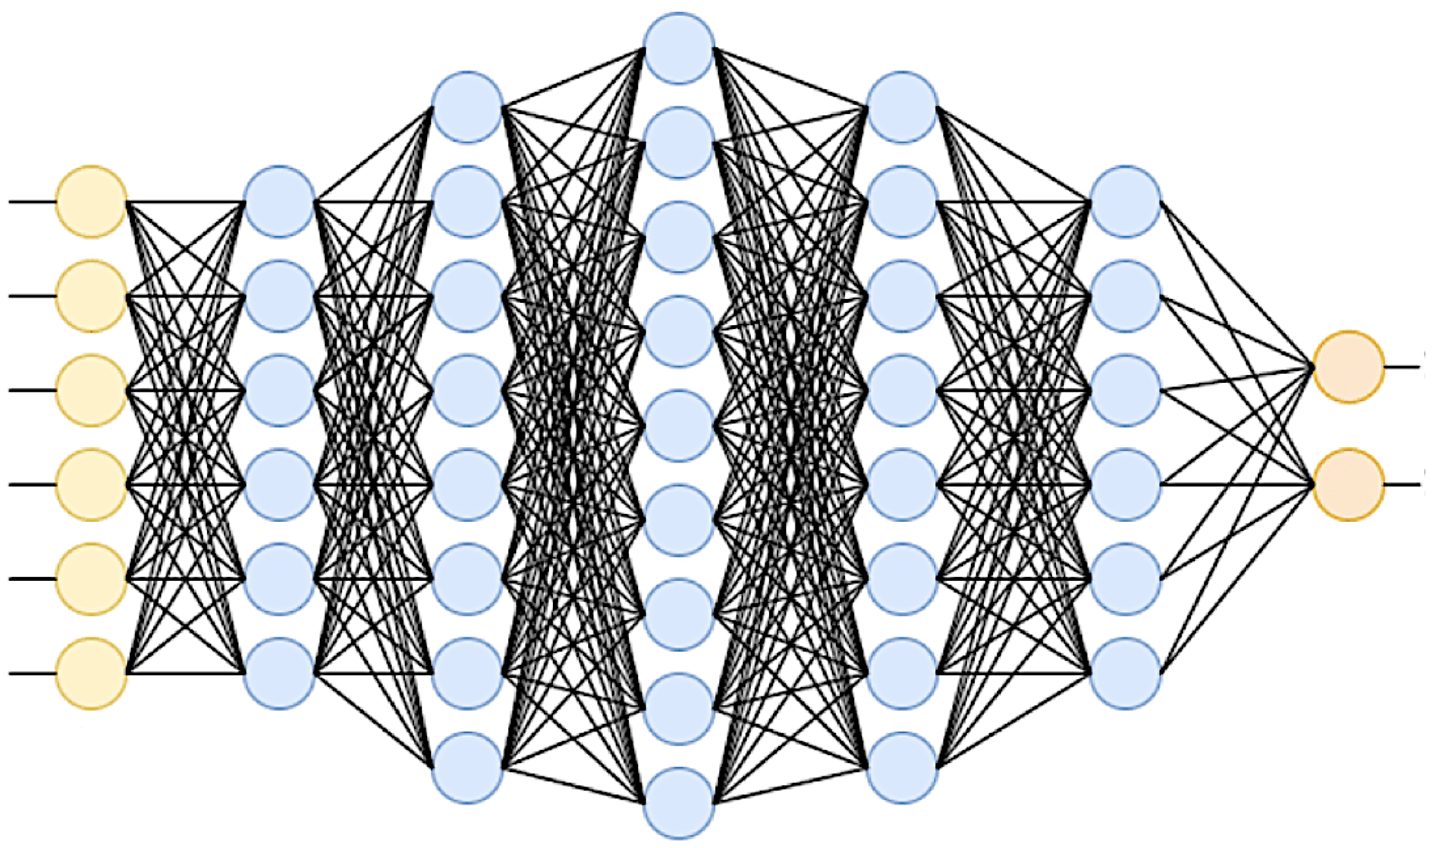
\includegraphics[keepaspectratio, scale=0.4]
 	{Figure/Deeplearning/dnn.png}
 		\caption{ディープニューラルネットワーク}
 		\label{dnn}
	\end{center}
\end{figure}
\section{グラフニューラルネットワーク}
深層学習では数値データのみでなく、画像認識や自然言語処理など様々なデータに対して目覚ましい成果を挙げている。その中で特に近年、グラフで表される構造データに対する研究が非常に盛んになっており、本研究において取り上げるグラフニューラルネットワーク\cite{gnnreview}もその一つである。グラフ構造データとは、オブジェクトの集合(ノード)を関係(エッジ)で結んだデータのことで、ノードのみが特徴量を持つ場合と、ノードとエッジの両方が特徴量を持つ場合がある。代表的には友人関係や論文の引用関係、化学化合物などをグラフデータとして構築することは有用であるとされており、データ間の相互関係を用いたモデリング・学習が可能であるため、高い表現力を持つことを強みとしている。グラフの種類は大きく分けてノードの次元が同じ同種グラフと、異なる次元のデータを扱う異種グラフの2種類に分けられる。更に、エッジが方向性を持っている有向グラフと無向グラフ、データが時系列で変化する動的グラフと変化しない静的グラフに分けられる。そしてこのようなグラフデータを扱うニューラルネットをグラフニューラルネットワーク(Graph Neural Network, GNN)という。グラフ構造や演算技術、目的とする課題によってGNNのネットワークモデルの種類は多岐にわたっており、以下では基本的なグラフでの演算や本論文に関連した幾つかの種類のモデルを取り上げる。\\
\subsection{メッセージパッシング}
GNNのアーキテクチャにおいて、グラフは集合$\mathcal{G} = (\mathcal{V}, \mathcal{E})$で構成されており、$\mathcal{V}$はノードの集合、$\mathcal{E}$はエッジの集合を表す。ニューラルネットワークの場合と同様にノードは特徴量を持っており、エッジも特徴量を持つことができる。図\ref{messagepass}にGNNにおける一般的な演算処理の流れ(メッセージパッシング)を示す。各ノードを$\mathbf{h}_i$とすると、隣接しているノードおよびその間のエッジの特徴量を集約し、ノードを更新$\mathbf{h}'_1$する。これによってエッジによって関連づけられたノード間で特徴量を更新していくことができる。エッジが特徴量を持つ場合は、エッジについても更新を行う。これらを数式にまとめると次のようになる。
\begin{align}
\mathbf{h}_{(i,j)} &= f_{edge}(\mathbf{h}_i, \mathbf{h}_j, x_{(i, j)})\\
\mathbf{h}'_i &= f_{node}(\mathbf{h}_i, \sum_{j\in \mathcal{N}_i}, \mathbf{h}_{(j, i)}, x_i)
\label{gnnm}
\end{align}
ここで、$\mathbf{h}_{(i,j)}$はエッジを、$x_i$はノードの特徴量を、$\mathcal{N}_i$は隣接しているノードの集合を表す。
\begin{figure}[H]
	\begin{center}
 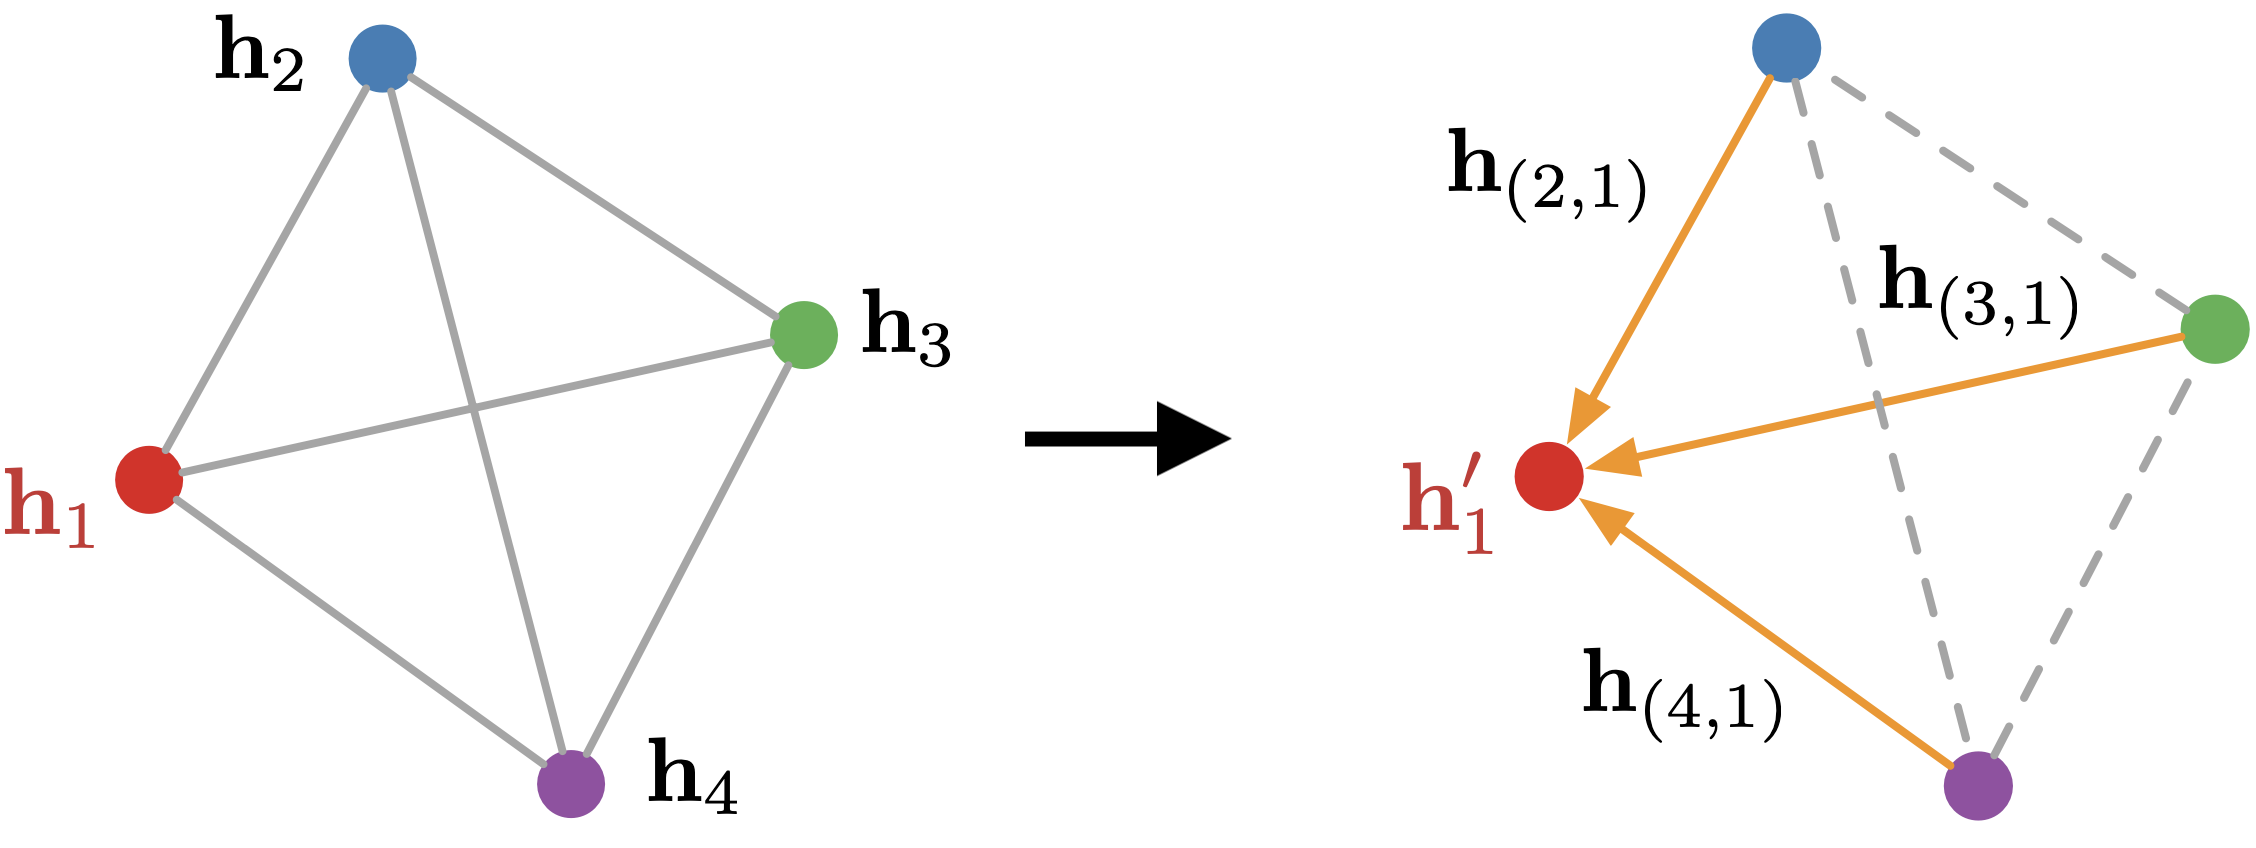
\includegraphics[keepaspectratio, scale=0.25]
 	{Figure/Deeplearning/messagepassing.png}
 		\caption{ (左) 4つのノードを持つ全結合グラフニューラルネットワーク。$h_i$はノード表現を表す。 (右) メッセージパッシングの処理。}
 		\label{messagepass}
	\end{center}
\end{figure}
\subsection{Graph Convolution Network (GCN)}
GCNとは、メッセージパッシングにおいて畳み込み(Convolution)を用いる手法である。一般的に機械学習における畳み込みは、あるフィルターを用いて対象と掛け合わせたものの和をとることで、周辺の情報を含ませることのできる処理であり、画像処理などにおいて広く用いられている。グラフの畳み込みにおいてはスペクトルによるアプローチと空間的なアプローチの2つがあり、以下ではそれぞれについて説明する。
\subsubsection{Spectral Graph Convolution}
スペクトルによる畳み込みは信号処理の考えに基づいたアプローチである。音声などの信号処理においては、関数をフーリエ変換によって周波数成分に変換し、ノイズ除去をして逆変換する。これをグラフデータに置き換えると、グラフラプラシアンの固有ベクトルが張る空間への変換・逆変換となる。グラフ信号を$\mathbf{x}$とすると、グラフフーリエ変換$\mathscr{F}(\mathbf{x})$、逆グラフフーリエ変換$\mathscr{F}^{-1}(\mathbf{x})$は次のように表される。
\begin{align}
\mathscr{F}(\mathbf{x}) &= \mathbf{U}^T\mathbf{x}\\
\mathscr{F}^{-1}(\mathbf{x}) &= \mathbf{U}\mathbf{x}
\end{align}
ここで、$\mathbf{U}$は正規化グラフラプラシアン$\mathbf{L}'$の固有ベクトル行列を表す。グラフラプラシアン$\mathbf{L}$は、グラフの隣接を表す隣接行列$\mathbf{A}$とグラフの各ノードに接続したノード数を対角成分にもつ次数行列$\mathbf{D}$を用いて、$\mathbf{L} = \mathbf{D}-  \mathbf{A}$で求められる実対称正方行列であり、正規化グラフラプラシアンは$\mathbf{L}' = \mathbf{I} - \mathbf{D}^{\frac{1}{2}} \mathbf{A} \mathbf{D}^{\frac{1}{2}}$とかける。\\
 これらを用いて、グラフにおけるSpectralな畳み込み演算は次のように定義される。
\begin{align}
\mathbf{g} \star \mathbf{x} &= \mathscr{F}^{-1}(\mathscr{F}(\mathbf{g}) \odot \mathscr{F}(\mathbf{x}))\\
&= \mathbf{U}(\mathbf{U}^T \mathbf{g} \odot \mathbf{U}^T \mathbf{x})
\end{align}
$\mathbf{g} \star \mathbf{x}$は畳み込み演算を、$\mathbf{U}^T \mathbf{g}$はスペクトルにおける畳み込みのフィルターを、$\odot$は要素ごとの積を行うアダマール積を表す。学習により更新される集合である$\mathbf{g}$に焦点を当ててより単純化すると、畳み込みは次のように書くことができる。\\
\begin{align}
\mathbf{g} \star \mathbf{x} &= \mathbf{U} \mathbf{g} \mathbf{U}^T \mathbf{x}
\end{align}
 上記のように、スペクトルによる畳み込みは一度の更新の中でグラフ構造の一部が全体に影響を与えるような演算であるという特徴を持っている。さらに、行列の次元が固定されてしまうことから異なる構造のグラフ間でパラメータを共有できないことや、行列の固有値分解など計算量が多くなってしまうという問題点がある。
\subsubsection{Spatial Graph Convolution}
グラフデータにおける畳み込みは空間的なメッセージパッシングの考えに基づいており、グラフ内の1つのノードが持っている特徴量に、隣接関係にあるノードの特徴量に重みをかけたものを加えていく。これによりノード自体の特徴量に加え、隣接関係や隣接ノードの特徴量の情報などを含んだ演算を行うことができる。メッセージパッシングにおける工夫に応じて様々な畳み込みのモデルが提案されているが、以下では最も一般的なモデルであるGraphSAGEについて述べる。\\
 GraphSAGE(Graph SAmple and aggreGatE)\cite{graphsage}では、隣接から特徴量をサンプリングして集約することで自身のノードを更新する。GraphSAGEにおける畳み込み演算は式\ref{gnnm}と同様に、次の式のように表される。\\
\begin{align}
&\mathbf{h}_{\mathcal{N}(v)}^k \leftarrow \mathrm{AGGREGATE}_k(\{ \mathbf{h}_u^{k-1}, \forall u \in \mathcal{N}(v) \})\\
&\mathbf{h}_v^k \leftarrow \sigma (\mathbf{W}^k \cdot \mathrm{CONCAT}(\mathbf{h}_v^{k-1}, \mathbf{h}_{\mathcal{N}(v)}^k))\\
&  (\forall k \in \{1, ..., K\}, \forall v \in \mathcal{V}) \nonumber
\end{align}
ここで、$K$は集約における隣接の深さを、$\mathbf{W}^k$は重みパラメータ行列を、$\sigma$は非線形関数を表しており、1式目$\mathrm{AGGREGATE}$で集約を、2式目$\mathrm{CONCAT}$で更新を行なっている。GraphSAGEはあらかじめサンプリングによって、隣接するノード数が異なる場合やグラフ構造が変わった場合にも畳み込み演算を行うことができ、さらに大規模なグラフ演算に対しては計算コストを改善することができる。
\begin{figure}[H]
	\begin{center}
 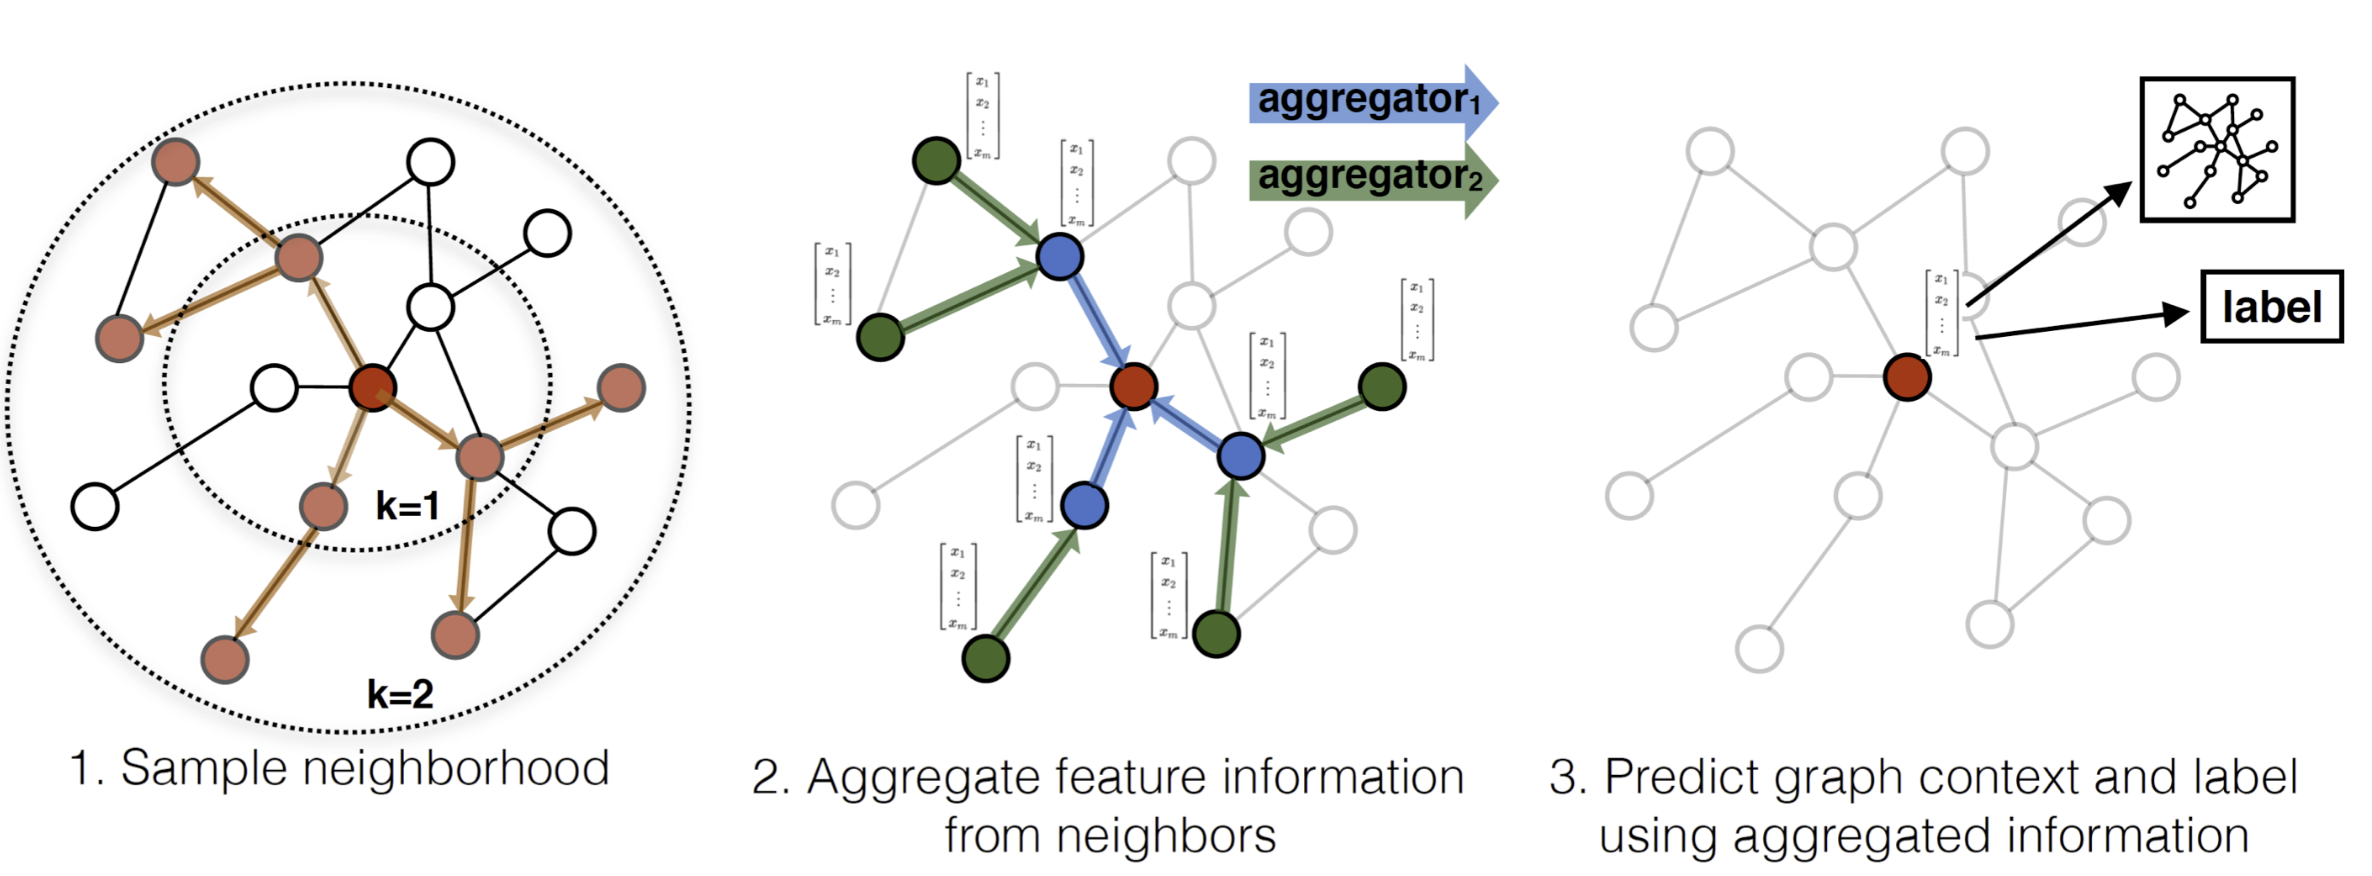
\includegraphics[keepaspectratio, scale=0.3]
 	{Figure/Deeplearning/sage.png}
 		\caption{GraphSAGEにおける処理(1. サンプリング, 2. 隣接からの集約, 3. 学習結果による推論)}
 		\label{sage}
	\end{center}
\end{figure}
\subsection{Graph Attention Network (GAT)}
\label{GATexplain}
深層学習ではAttentionという、データの中でも特に有益な場所に重み付けを行う手法があり、自然言語処理の分野などにおいてよく用いられている。Attention機構では各ノードに対して重要度を表す重みを導入し、それらを掛けた和をとることで必要な場所に注目(attention)を向けることができる。Attentionをグラフ学習に適用したものが、Graph Attention Networks (GAT) \cite{gat} である。GATでは、重みパラメータ$\mathbf{W}$に加えて隣接したノードの重要度を表すattention係数$\alpha_{ij}$を導入して、ノードの特徴量の更新を以下のように行う。
\begin{align}
\mathbf{h} = \sigma (\sum_{j \in \mathcal{N}_i} \alpha_{ij} \mathbf{W} \mathbf{h}_i )
\end{align}
ここで、$\alpha_{ij}$はattention処理$\mathbf{a}$を用いて、次のように表される。
\begin{align}
\alpha_{ij} &= \mathbf{a}(\mathbf{W}\mathbf{h}_i, \mathbf{W}\mathbf{h}_j)\\
 &= \frac{e^{LeakyReLU(\mathbf{a}^T [ \mathbf{W}\mathbf{h}_i \parallel \mathbf{W}\mathbf{h}_j ])}}{\sum_{\mathcal{N}_i} e^{LeakyReLU(\mathbf{a}^T [ \mathbf{W}\mathbf{h}_i \parallel  \mathbf{W}\mathbf{h}_j ])}}
\label{gatattention}
\end{align}
 GATではattention処理に1層のニューラルネットワークを用いており、$\mathbf{a}$として学習の重みベクトルを用いている。式\ref{gatattention}においては全ノード間で正規化して確率値を出力するためのsoftmax関数の適用と、活性化関数 (Leaky ReLU) の適用を行っている。($\cdot^T$は転置を、$\parallel$はテンソルのconcatenateを表す。)GATは、隣接に任意の重みを割り当てることから次数の異なるノードにも適応可能であり、未知のグラフ構造にも一般化することができる。
\begin{figure}[H]
	\begin{center}
 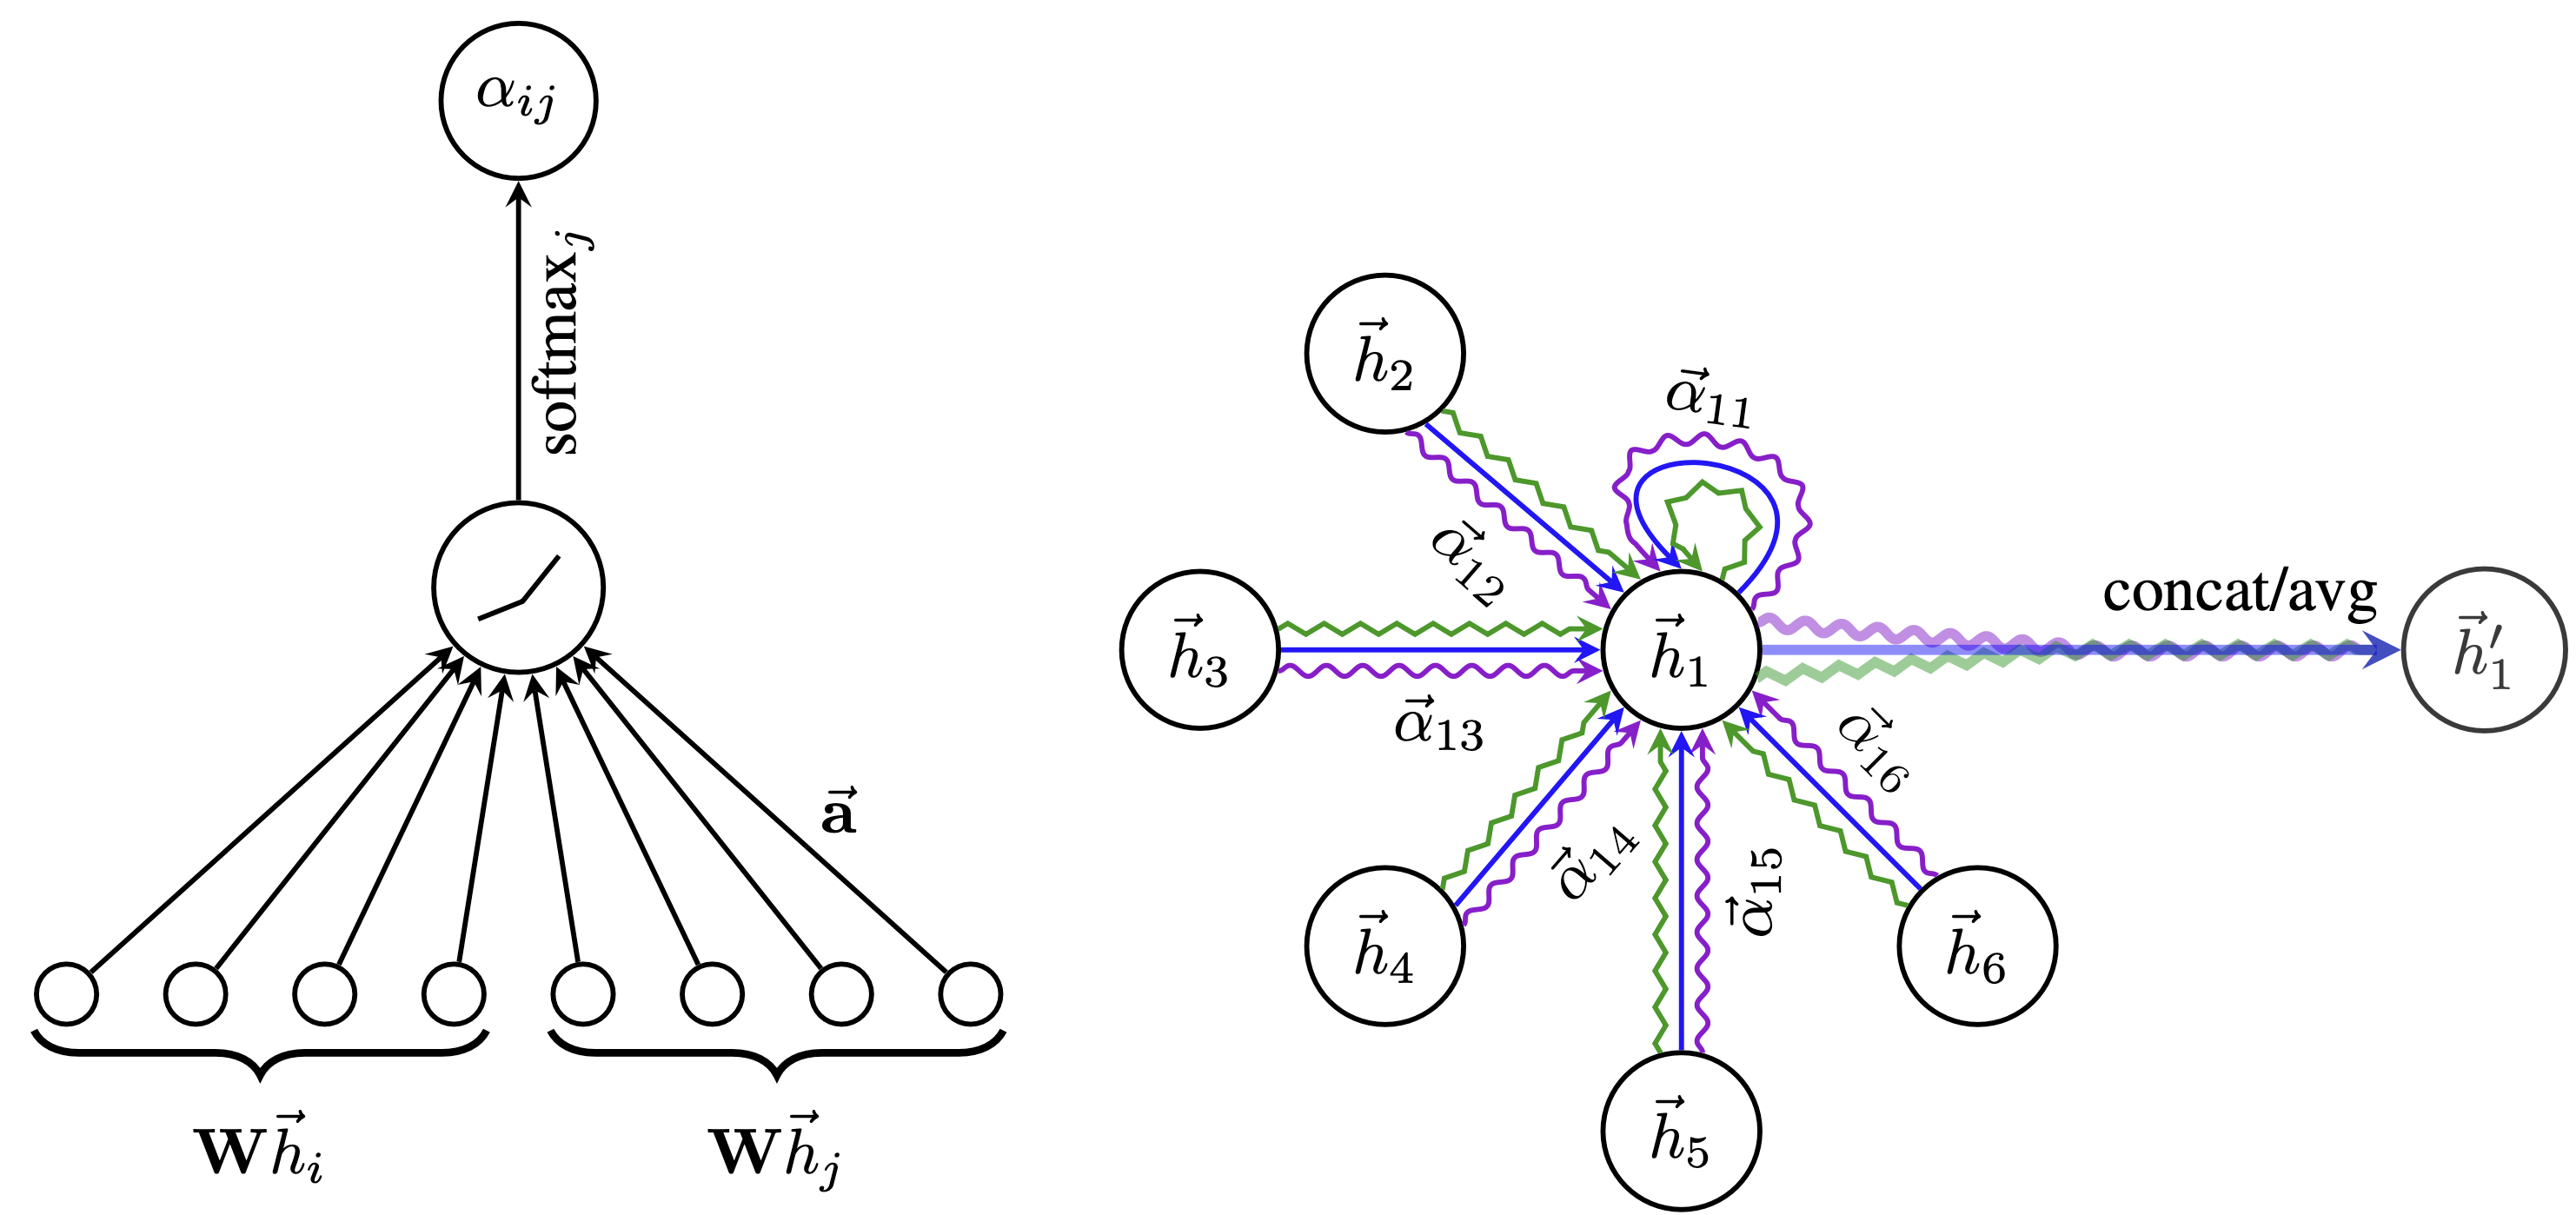
\includegraphics[keepaspectratio, scale=0.25]
 	{Figure/Deeplearning/gat.png}
 		\caption{ (左) 重みベクトル$\mathbf{a}$を用いたAttention処理。 (右) 1つのノード$\mathbf{h}_1$に対する隣接ノード$\mathbf{h}_{\neq 1}$のAttentionと、ノード特徴量の更新$\mathbf{h'}_1$}
	\end{center}
\end{figure}
 % !TEX root = ../MasterThesis_Onoe.tex
% 上記はただのコメントではなく親ファイルの場所を教えているので
% 消してしまうとファイルごとのタイプセットができなくなるので注意。
% 親ファイル名を変更したときはここも変更する。

\externaldocument{Deeplearning}

\chapter{深層学習を用いたジェットフレーバー識別} \label{sec:Flavortagging}
本章では、深層学習を用いて開発したジェットフレーバー識別アルゴリズムについて述べる。まず5.1節では、フレーバー識別に関係する事象の詳細についてや、現在ジェットフレーバー識別に用いられているLCFIPlusについて述べる。次に3.2節で、今回のアルゴリズムの評価において使用したMCシミュレーションデータについて述べる。またシミュレーションデータには深層学習における精度を上げるために前処理を行なっており、これについても述べる。そして5.3節、5.4節それぞれでディープニューラルネットワーク、グラフニューラルネットワークによる実装について述べ、5.5節でLCFIPlusと比較を行って学習の性能について議論する。
%\section{ジェットフレーバー識別アルゴリズム}
%\subsection{事象について}
\section{イベントサンプルと先行研究}
本研究では、MCイベントジェネレーターであるwhizardによる事象生成を行い、ILD検出器のフルシミュレーションを使用したデータを用いてフレーバー識別を行った。シミュレーションデータについての詳細を表\ref{inputdatas}に示す。
\begin{table}[H]
 \centering
 \begin{tabular}{ c c }
 \hline
 イベントジェネレーター & whizard\\
 シミュレーション & ILD Full simulation\\
 検出器モデル & ILD\_l5\_250GeV\_v02-02\\
 反応過程 & $e^+e^- \rightarrow \nu \bar{\nu} h \rightarrow \nu \bar{\nu} b \bar{b} / c \bar{c} / q \bar{q} (q = u,d,s)$\\
 重心系エネルギー & 250$\mathrm{GeV}$ \\
 ISR & なし\\
 ビーム偏極 & なし\\
 \hline
  \end{tabular}
  \label{inputdatas}
  \caption{シミュレーションデータの性質}
\end{table}
\subsection{LCFIPlusにおけるフレーバー識別}
LCFIPlusのフレームワークでは、フレーバー識別は崩壊点検出、ジェットクラスタリングの後に行われる。フレーバー識別は、飛跡や崩壊点の特徴量をもとにROOTのTMVAパッケージにおけるBoosted Decision Trees (BDTs) を用いて識別が行われる。このBoosted Decision Treesは、複数のモデルを組み合わせて全体的な性能を向上させるアンサンブル学習 (Boosting) と、入力された特徴量に基づいてデータをクラスに分割していく決定木 (Decision Tree) の手法を組み合わせたものであり、複数の弱い決定木モデルを組み合わせて決定木の精度を向上させる機械学習手法である。データは、初めに崩壊点の数で場合分けが行われ、次ページに示す、表\ref{lcfiplusin}にある入力変数をもとに、最終的に各ジェットをb/c/udsの3つに分類する学習を行う。
\begin{table}[H]
 \centering
 \small
  \begin{tabular}{ l | l }
   \hline
   変数名 & 説明\\
   \hline \hline
%   nvtx & 崩壊点の数\\
   trk1d0sig & $d_0$のsignificanceが最も高い飛跡の$d_0$\\
   trk2d0sig & $d_0$のsignificanceが2番目に高い飛跡の$d_0$\\
   trk1z0sig & $z_0$のsignificanceが最も高い飛跡の$d_0$\\
   trk2z0sig & $z_0$のsignificanceが2番目に高い飛跡の$d_0$\\
   trk1pt & $d_0$が最も大きい飛跡の横方向運動量\\
   tkr2pt & $d_0$が2番目に大きい飛跡の横方向運動量\\
   jprobr & 全飛跡を用いたr-$\phi$平面での結合確率\\
   jprobr5sigma & 5$\sigma$以上のパラメータを持つ全飛跡を用いたr-$\phi$平面での結合確率\\
   jprobz & 全軌跡を用いたz軸射影での結合確率\\
   jprobz5sigma & 5$\sigma$以上のパラメータを持つ全飛跡を用いたz軸射影での結合確率\\
   d0bprob & 全飛跡に対してb,c,udsフレーバーの$d_0$分布を用いた$d_0$のb-クォーク確率の積\\
   d0cprob & 全飛跡に対してb,c,udsフレーバーの$d_0$分布を用いた$d_0$のc-クォーク確率の積\\
   d0qprob & 全飛跡に対してb,c,udsフレーバーの$d_0$分布を用いた$d_0$のuds-クォーク確率の積\\
   z0bprob & 全飛跡に対してb,c,udsフレーバーの$z_0$分布を用いた$d_0$のb-クォーク確率の積\\
   z0cprob & 全飛跡に対してb,c,udsフレーバーの$z_0$分布を用いた$d_0$のc-クォーク確率の積\\
   z0qprob & 全飛跡に対してb,c,udsフレーバーの$z_0$分布を用いた$d_0$のuds-クォーク確率の積\\
   nmuon & ミューオンの数\\
   nelectron & 電子の数\\
   trkmass & $d_0/z_0$が5$\sigma$を超える全飛跡の質量\\
   1vtxprob & 崩壊点に関連した全飛跡を結合した時の崩壊点確率\\
   vtxlen1 & ジェット内の2番目の崩壊点の崩壊長\\
   vtxlen2 & ジェット内の3番目の崩壊点の崩壊長\\
   vtxlen12 & ジェット内の2番目の崩壊点と3番目の崩壊点の距離\\
   vtxsig1 & vtxlen1のsignificance\\
   vtxsig2 & vtxlen2のsignificance\\
   vtxsig12 & vtxlen12を2番目の崩壊点と3番目の崩壊点の共分散行列の和の誤差で割った値\\
   vtxdirang1 & 運動量と2番目の崩壊点の変位との間の開き角\\
   vtxdirang2 & 運動量と3番目の崩壊点の変位との間の開き角\\
   vtxmult1 & 2番目の崩壊点に含まれる飛跡数\\
   vtxmult2 & 3番目の崩壊点に含まれる飛跡数\\
   vtxmult & secondary vertexを構成するために用いられる飛跡の数\\
   vtxmom1 & 2番目のの頂点に結合された全飛跡の運動量のベクトル和\\
   vtxmom2 & 3番目の頂点に結合された全飛跡の運動量のベクトル和\\
   vtxmass1 & 飛跡の四元運動量の和から計算される2番目の崩壊点質量\\
   vtxmass2 & 飛跡の四元運動量の和から計算される3番目の崩壊点質量\\
   vtxmass & secondary vertexを構成する全 飛跡の四元運動量の和から計算される崩壊点質量\\
   vtxmasspc & primary/secondary vertexの誤差行列で許容可能なpt補正を行なった崩壊点質量\\
   vtxprob & 崩壊点が形成される確率\\
   \hline
  \end{tabular}
  \caption{LCFIPlusにおけるフレーバー識別の入力変数}
 \label{lcfiplusin}
\end{table}
\section{ディープニューラルネットワークによる実装}
本節では、ディープニューラルネットワーク (多層ニューラルネットワーク) によるフレーバー識別の実装について述べる。
\subsection{実装目的}
フレーバー識別では、シグナル効率に対して排除できる背景事象の割合が多くなるほど、ヒッグスなどの物理解析において有利であるため、その性能が非常に重要である。LCFIPlusにおいて実装されているBDTsは、崩壊点やジェットの特徴量の場合分けによって分類を行うため、ツリー構造が視覚化されており解釈が容易である。一方で、BDTsの場合分けにおける閾値は人の手で定める必要があり、ILCのフレーバー識別のようなデータが高次元で複雑なタスクに対しては、より複雑な表現学習の方が適している可能性がある。さらにBDTsにはノイズに敏感である点や、ツリー数が多くなると過学習を起こす点など問題点もある。そこで本研究では、フレーバー識別の更なる性能向上を目的にディープニューラルネットワークによる実装を行った。ディープニューラルネットワークでは、データから複雑な表現を自動的に学習することができる。そのため、より最適化したモデルの獲得を目指すため、ディープニューラルネットワークでの実装を行った。
\subsection{入力変数とネットワークアーキテクチャ}
学習の入力変数は、LCFIPlusにおいて用いた変数 (表\ref{dnnin}) と同様の変数を使用した。また、学習値に対しては前処理を行い、0付近の値が多い変数や値幅が大きい変数が存在したため、各変数に対して対数変換や正規化を実行した。また出力もLCFIPlusと同様にbフレーバー、cフレーバー、udsフレーバーとした。\\
ネットワークには図\ref{dnnmodel}のように最も単純な全結合層を用いたニューラルネットワークを採用した。さらに、過学習を抑制するためにバッチ正規化を各全結合層の後に行い、活性化関数には勾配消失への対策として全てLeakyReLU関数を使用した。損失関数には分類問題に適した交差エントロピーを用い、最適化アルゴリズムにはAdamを学習率0.01で使用した。また学習率は25 epoch(学習データでの学習回数)ごとに0.1倍させ、学習の安定化を目的に学習率を減衰させた。表\ref{dnnsetting}に学習におけるハイパーパラメータをまとめる。また、上記のネットワークは深層学習ライブラリであるPyTorchを用いて実装を行なった。PyTorchはPythonで使用可能なのライブラリであり、高速な数値計算を行うためのGPUサポートや、動的な計算グラフを導入しているため実行時コンパイル (Define-by-Run) という特徴を持っている。
\begin{figure}[H]
	\begin{center}
 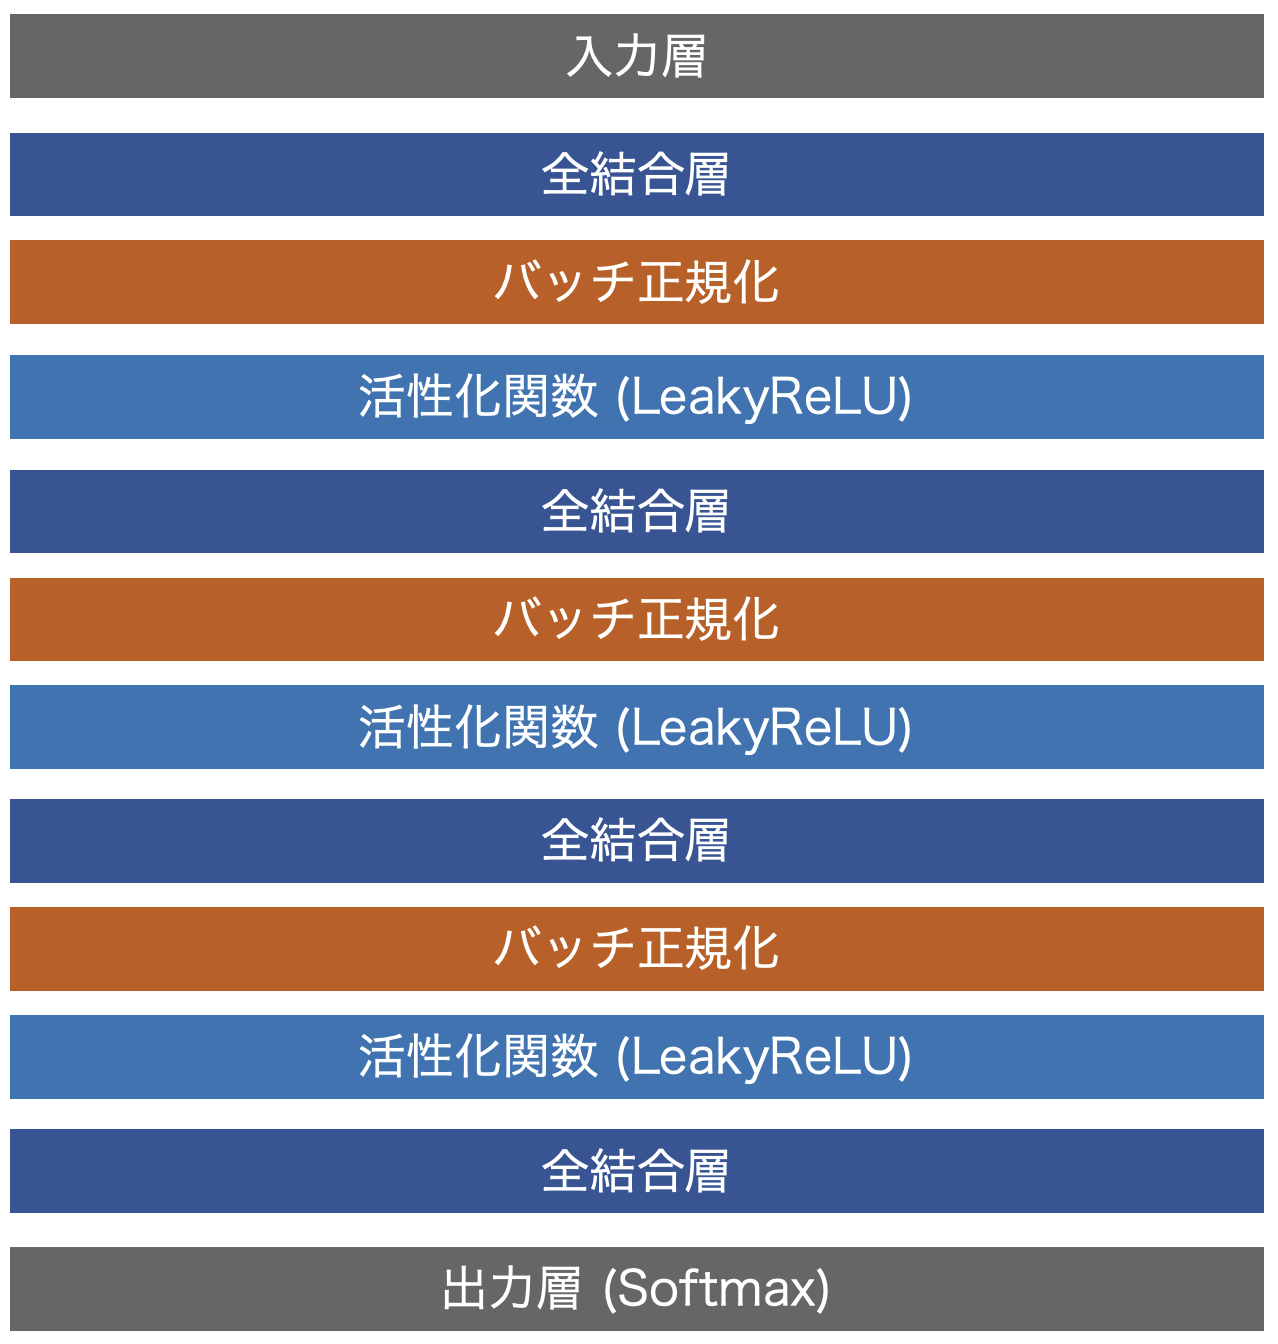
\includegraphics[keepaspectratio, scale=0.5]
 	{Figure/Flavortagging/dnn.png}
 		\caption{フレーバー識別のためのディープニューラルネットワークの概略図}
 		\label{dnnmodel}
	\end{center}
\end{figure}
\begin{table}[H]
 \centering
  \begin{tabular}{ l  l }
   \hline
   ノード数 & (124, 124, 124)\\
   活性化関数 & ReLU関数\\
   損失関数 & 交差エントロピー\\
   最適化アルゴリズム & Adam\\
   学習率 & 0.01 (25epochあたり0.1倍)\\
   エポック数 & 100\\
   バッチサイズ & 1024\\
   \hline
  \end{tabular}
  \caption{ディープニューラルネットワークにおけるハイパーパラメータ}
  \label{dnnsetting}
\end{table}
\subsection{ハイパーパラメータの最適化}
記入予定
\subsection{学習評価}
学習における損失関数の値と識別精度を図\ref{dnnoutput}に示す。100epochの学習によって、損失関数の値は降下したのちおおよそ安定しており、学習精度はおよそ$82.5\%$となっている。また、図\ref{dnncm}に混合行列を示す。混合行列とは、分類問題で出力された結果をまとめた表であり、縦軸 (行) が実際の答えを横軸 (列) が学習結果を表していて、実際の答えごと (行) に正規化されている。そのため、左上から右下の対角成分が実際の答えと学習結果が一致している割合を表しており、図\ref{dnnoutput}における学習精度は$(学習精度) = (対角成分の和) / (全成分の和)$として求められる。図\ref{dnncm}より、ディープニューラルネットワークではcジェットについてはudsジェットと識別しにくいことがわかる。\\
\begin{figure}[H]
	\begin{center}
 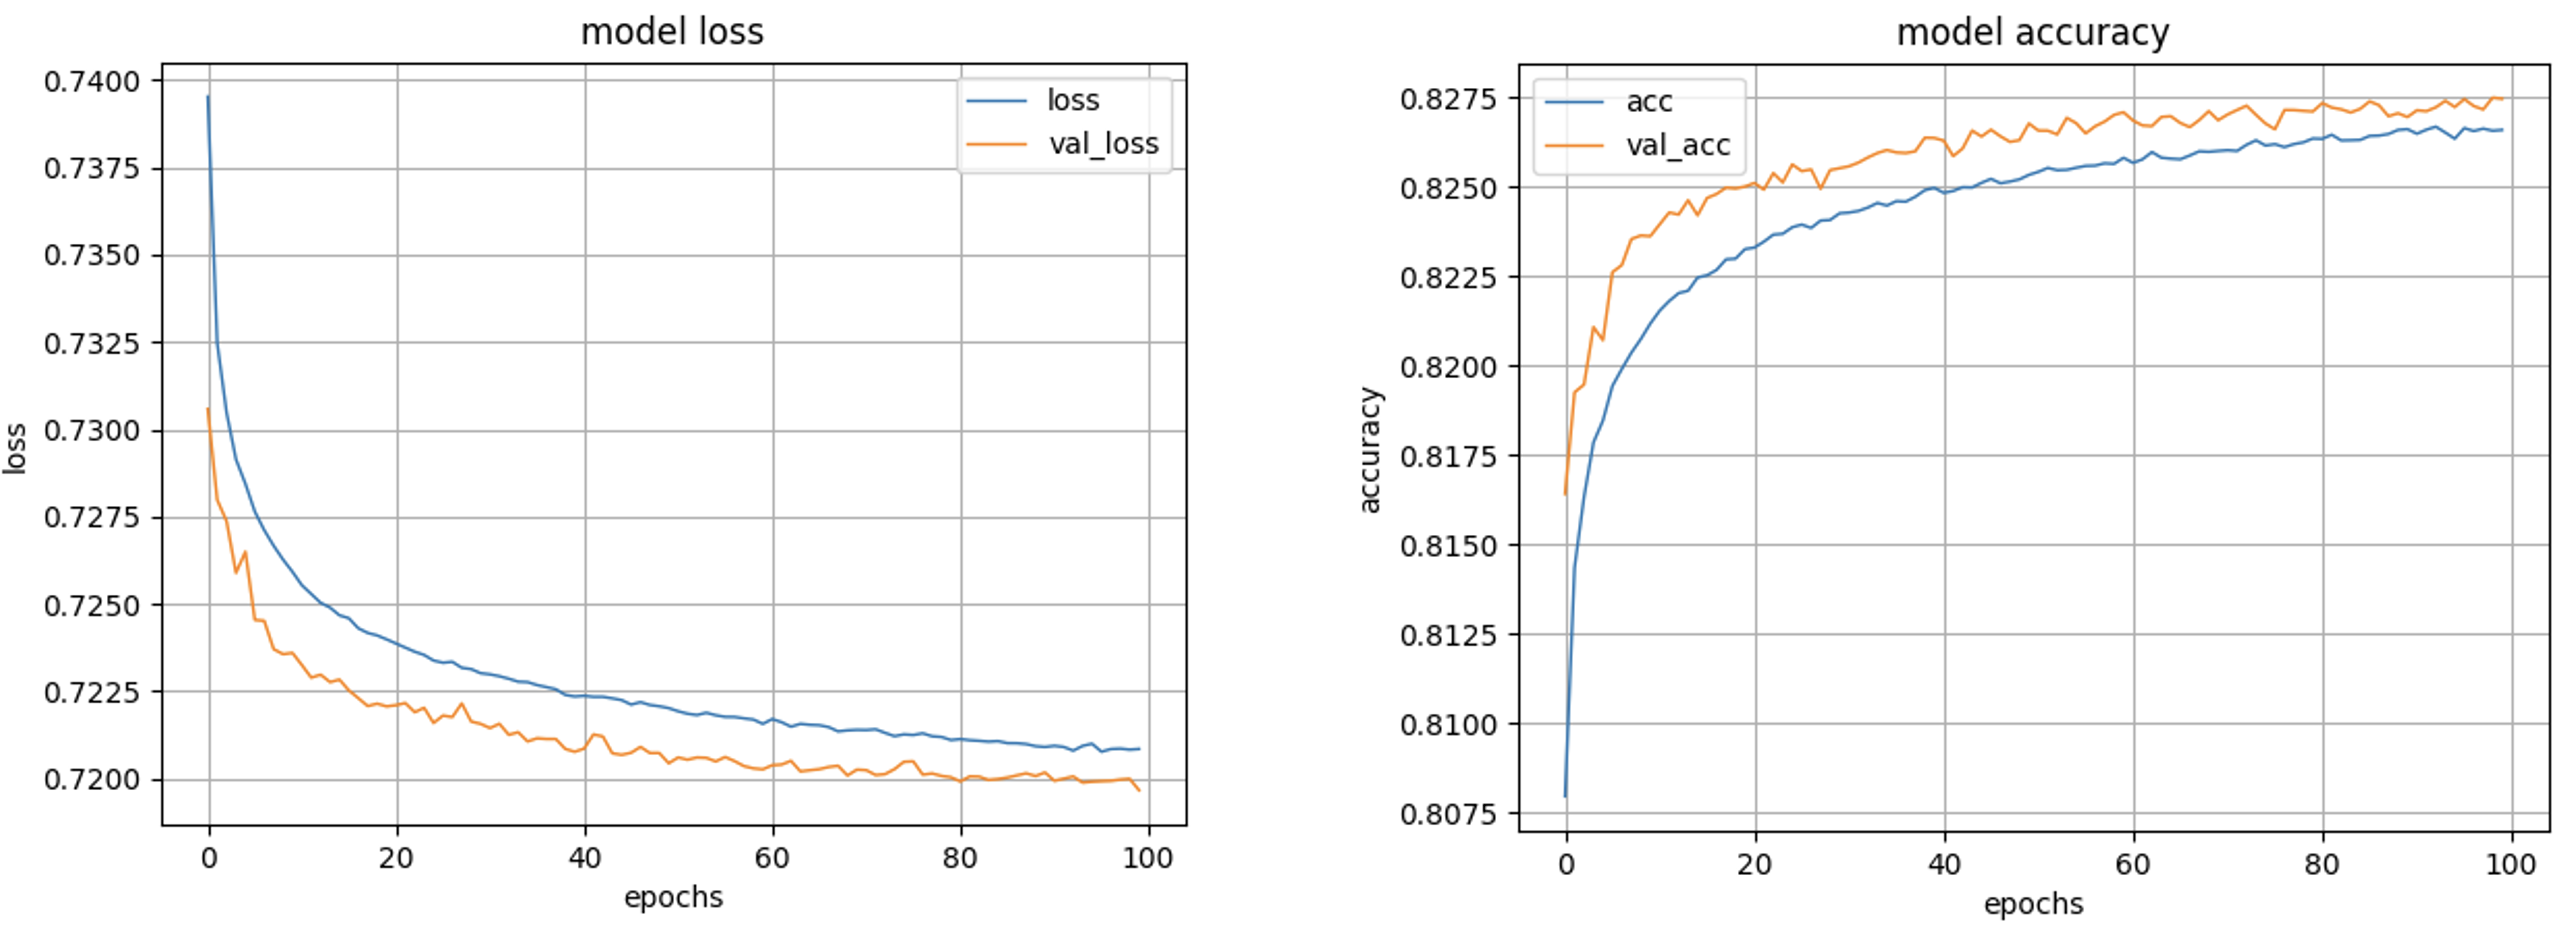
\includegraphics[keepaspectratio, scale=0.3]
 	{Figure/Flavortagging/dnnout.png}
 		\caption{(左)学習の経過における損失関数。(右)学習の経過における学習精度}
 		\label{dnnoutput}
	\end{center}
\end{figure}
\begin{figure}[H]
	\begin{center}
 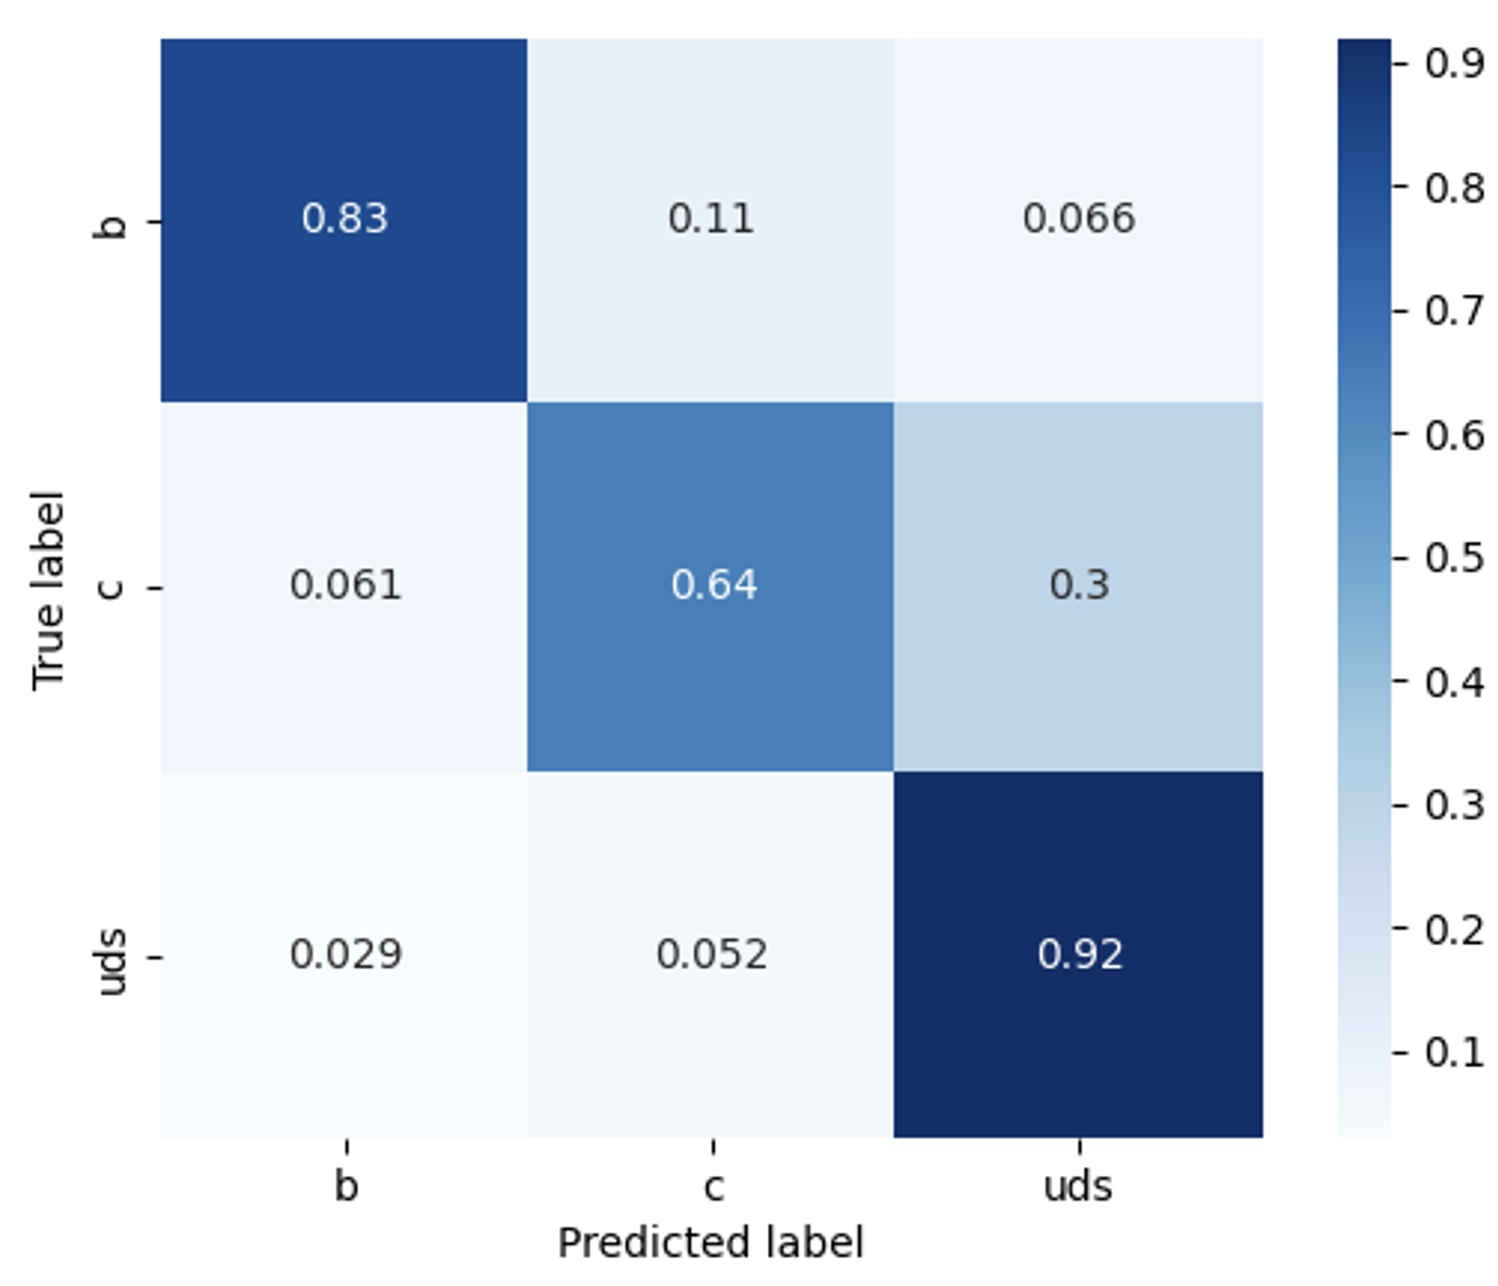
\includegraphics[keepaspectratio, scale=0.2]
 	{Figure/Flavortagging/dnncm.png}
 		\caption{ディープニューラルネットワークの学習における混合行列。縦軸が実際の答えを、横軸が学習結果を表している。}
 		\label{dnncm}
	\end{center}
\end{figure}
次に、LCFIPlusとの比較を示す。本アルゴリズムのモデルの出力値は1つのジェットに対してそれぞれのフレーバーである確率値が得られる。そして、物理解析においてはフレーバー識別の効率が重要であり、識別効率 (= フレーバーをある確率値で決定した場合の正しい認識率) に対して背景事象と誤認識してしまう割合が少なくなることが望ましい。図\ref{dnneff_b}, \ref{dnneff_c}はb/cジェットの識別効率のプロットを
%、表\ref{dnneff80}は識別効率を$80\%$ (Tagging Efficiency = 0.8) に固定したときの背景ラベルの識別効率の割合を
示している。bジェットの識別効率はLCFIPlusと比較して劣っており、特に識別効率$80\%$における識別割合は、LCFIPlusがcジェットの識別割合が$7.3\%$、udsジェットの識別効率が$0.74\%$であるのに対して、ディープニューラルネットのcジェットの識別割合は$20\%程度$、udsジェットの識別効率は$2\%程度$と、udsジェットの識別割合は30倍近く高くなっている。一方でcジェットの識別効率は識別効率$80\%$において、LCFIPlusがbジェットの識別割合が$22\%$、udsジェットの識別効率が$24\%$であるのに対して、ディープニューラルネットのbジェットの識別割合は$数\%程度$、udsジェットの識別効率は$24\%程度$と、bジェットの背景割合は半分以下になっている。本来フレーバー識別はb、cクォークの寿命が長いという特徴を活かして識別するという発想にあるため、崩壊点に関する変数で線形にモデリングしたBDTsでは、cジェットよりもbジェットの方が識別効率が高くなっている。一方でディープニューラルネットワークでは、関係性が逆転している。機械学習アルゴリズムの性能はデータの特性やタスクの種類に大きく依存するため、同じデータを用いていてもアルゴリズムが異なる場合、同じタスクに対する学習特性は異なることがある。今回の場合ではcジェットの識別において、ディープニューラルネットワークでデータ内の複雑な関係を処理できたため、このような結果になったと考えることができる。
\begin{figure}[H]
	\begin{center}
 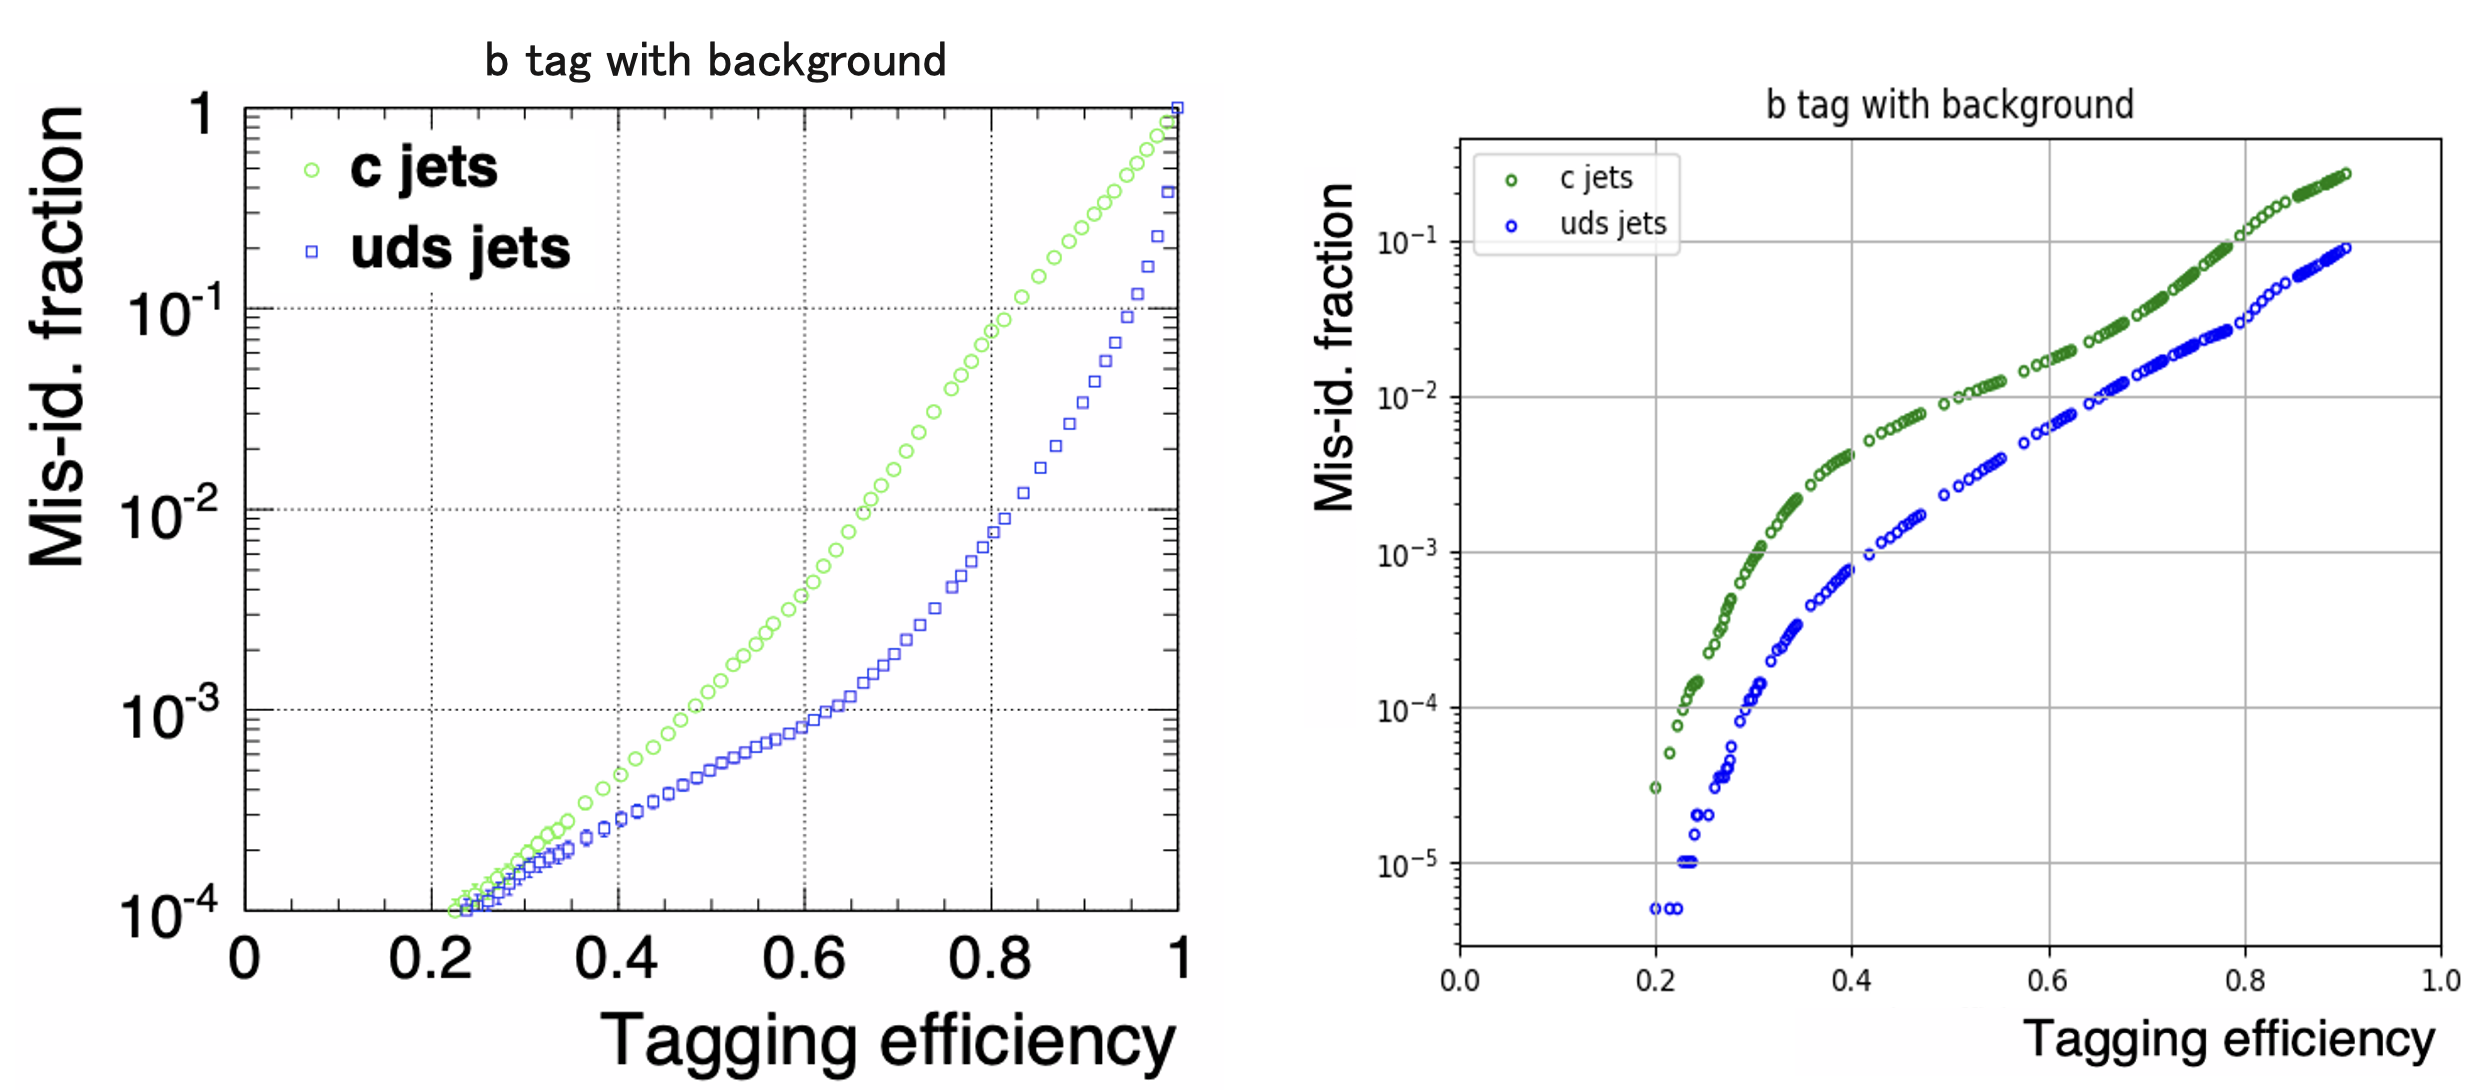
\includegraphics[keepaspectratio, scale=0.3]
 	{Figure/Flavortagging/dnneff_b.png}
 		\caption{LCFIPlus(左)とディープニューラルネットワーク(右)によるbフレーバージェットの識別効率の比較。緑:bジェットに対するcジェットの識別効率、青:bジェットに対するudsジェットの識別効率を示している。}
 		\label{dnneff_b}
	\end{center}
\end{figure}

\begin{figure}[H]
	\begin{center}
 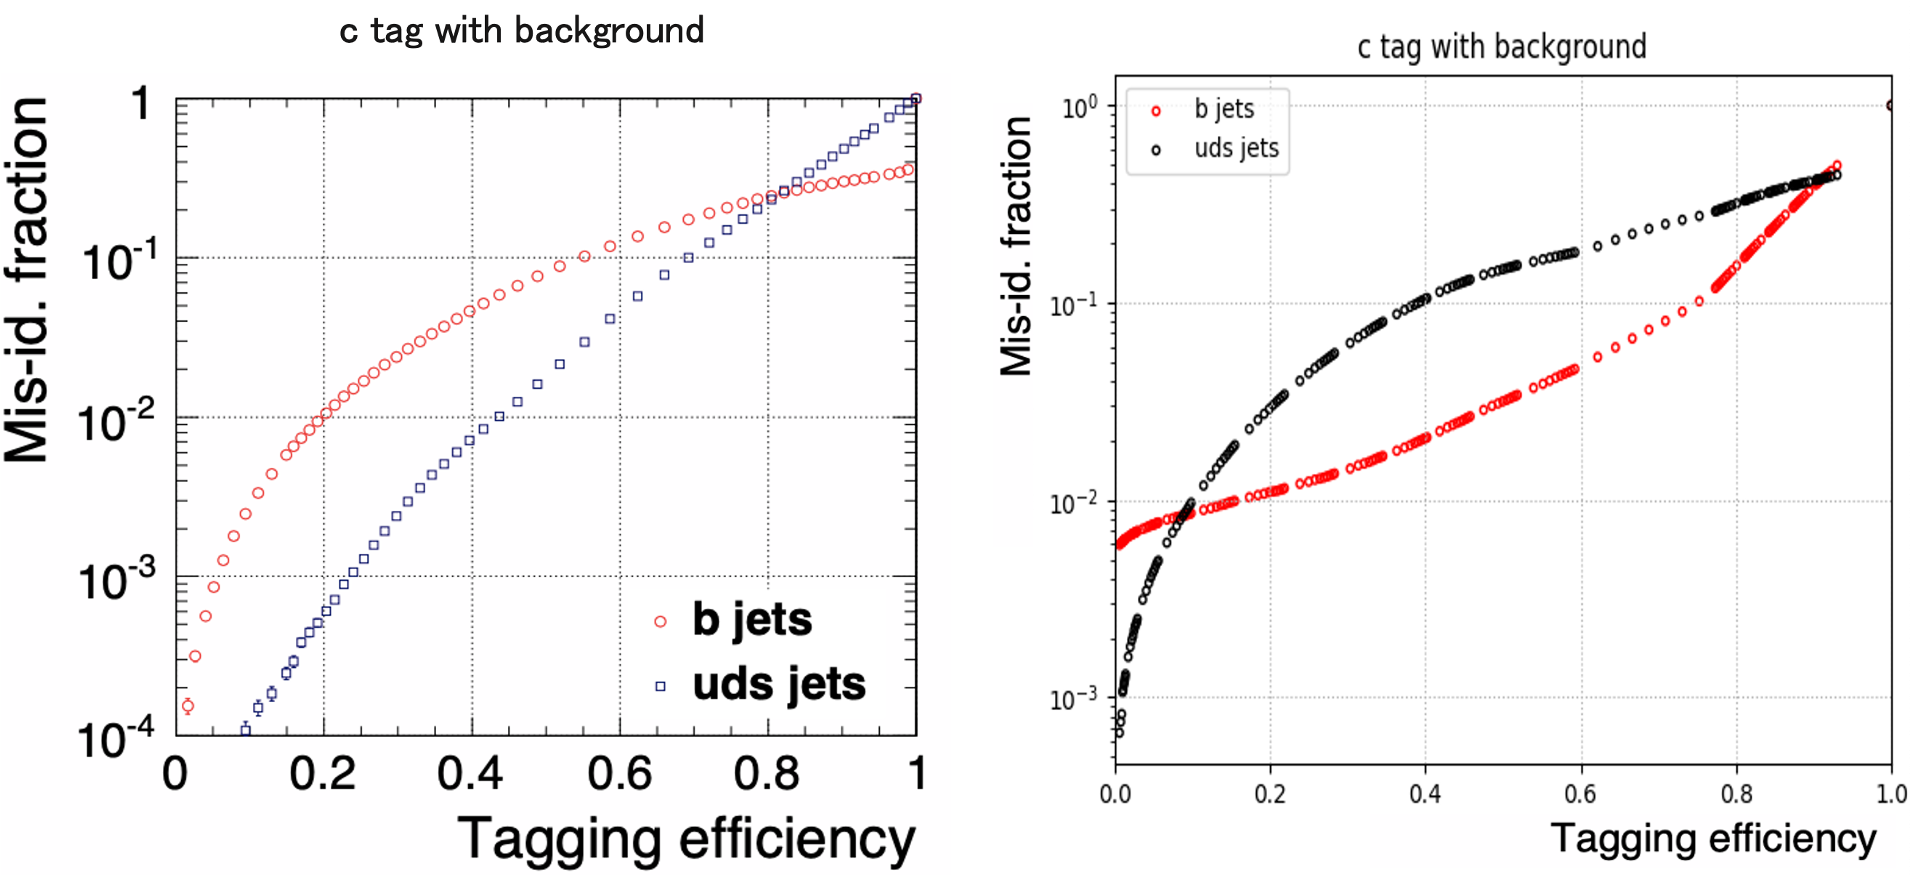
\includegraphics[keepaspectratio, scale=0.3]
 	{Figure/Flavortagging/dnneff_c.png}
 		\caption{LCFIPlus(左)とディープニューラルネットワーク(右)によるcフレーバージェットの識別効率の比較。赤:cジェットに対するbジェットの識別効率、黒:cジェットに対するudsジェットの識別効率。}
 		\label{dnneff_c}
	\end{center}
\end{figure}
%\begin{comment}
\begin{table}[H]
 \centering
  \begin{tabular}{ |c|c|c|c|}
   \toprule
   \multirow{2}{*}{識別効率=0.8} & \multirow{2}{*}{背景ジェット} & \multicolumn{2}{|c|}{誤認率} \\
    & & LCFIPlus & DNN\\ \cline{3-4} 
    \midrule
    \midrule
   \multirow{2}{*}{bジェット} & cジェット & 0.073 & $\sim$ 0.2\\ \cline{2-2} 
   & udsジェット & 0.0074 & $\sim$ 0.02 \\ \cline{1-2} 
   \multirow{2}{*}{cジェット} & bジェット & 0.22 & $\sim$ 0.7\\ \cline{2-2} 
   & udsジェット & 0.24 & $\sim$ 0.24\\
   \bottomrule
  \end{tabular}
  \caption{識別効率 (Tagging Efficiency) に対するジェット誤認率 (Mis-id fraction)}
  \label{dnneff80}
\end{table}
%\end{comment}

\section{グラフニューラルネットワークによる実装}
本節では、グラフニューラルネットワークによるフレーバー識別の実装について述べる。
\subsection{実装目的}
5.3節におけるディープニューラルネットワークの実装では、一部で精度の向上が見られたものの顕著な識別精度の改善はなかった。そこで、ILCのフレーバー識別により最適化した学習を行うために、より高い表現力を持つグラフニューラルネットワークによる実装を考えた。ILCにおけるジェットの物理現象の振る舞いはトポロジカルな構造を持っており、またジェット内の飛跡同士は崩壊点を共有するものが存在している。そのため、グラフデータによってトポロジカルな構造を再現し、データ間の相互関係を活かした学習を行うことで、高い表現力によるアルゴリズムモデルの最適化を目指した。\\
さらにグラフニューラルネットワークの実装では、データをグラフ構造化する上でジェットの内部構造を理解するようなモデルを構築する必要があり、これを補助学習としたアルゴリズムの統合が可能であると考えた。つまり、これまでのようなプロセスを分離した高度なアルゴリズムではなく、1つのアルゴリズム内で飛跡に関する入力変数のみから、飛跡の分類や崩壊点の予想と同時にジェットフレーバーの識別を行うことを可能とするものである。これによって、情報損失を少なくすることで性能の向上を目指すとともに、アルゴリズム調整の単純化や、飛跡の分類結果など将来的に他のアプリケーションに利用可能な情報の生成までもを期待することができる。
\subsection{飛跡によるグラフデータセット}
ILCにおけるジェットの振る舞いを再現するため、本アルゴリズムでは1つのジェットに対して、に飛跡をノードとし全ノードがエッジによって結ばれる1つの同種グラフを構築した。(図\ref{1graph})各ノードは表\ref{gnninput}に挙げる特徴量を入力変数として持ち、エッジは特徴量を持たないものとした。ノードの特徴量には、飛跡に関するパラメータ (Appendix) を用いた。入力データの生成のため、まず250GeVのILDフルシミュレーションにおける$e^+e^- \rightarrow \nu \nu H$事象を使用し、飛跡再構成を行った。続いてLCFIPlusのVertex Fitterプロセスによって、飛跡対が結合する確率値を得た。またシミュレーションにおける答えをもとに3つの学習に対して次のような答えラベルを準備した。それぞれ、ノードの答えラベルは飛跡がどのフレーバージェットのどのvertexから来たものであるのか、エッジの答えラベルは飛跡対が同じ崩壊点を共有するかのバイナリ形式、グラフの答えラベルはどのフレーバーであるのかを答えとした。各学習の答えラベルについて表\ref{gnnoutput_n}$\sim$表\ref{gnnoutput_g}にまとめる。また、入力変数には前処理を行った。さらにデータ数は答えラベル間で偏りがあり、ノードに関するラベルあたりのデータ数\ref{node_imb}はPrimary Vertexを由来とする飛跡が突出して多かったため、比の逆数を重みとして損失関数で考慮することで対応した。また、本アルゴリズムの実装はPyTorchとグラフニューラルネットワーク向けのグラフ構造を扱うためのPyTorchライブラリであるPyTorch Geometricを用いて行なった。
\begin{figure}[H]
	\begin{center}
 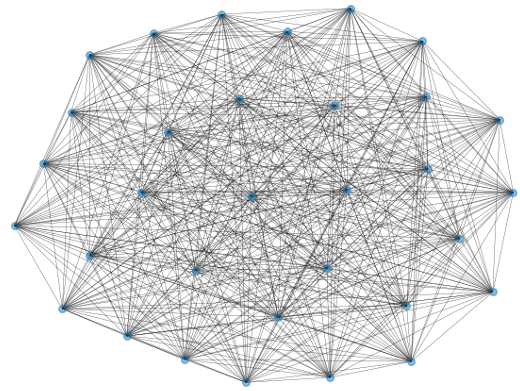
\includegraphics[keepaspectratio, scale=0.5]
 	{Figure/Flavortagging/graphexample.png}
 		\caption{今回の学習に用いたグラフデータの一例。ノードは飛跡を、グラフ全体が1つのジェットに対応する。}
 		\label{1graph}
	\end{center}
\end{figure}

\begin{table}[H]
\centering
 \begin{tabular}{ l  l }
 \hline
 変数名 & 説明\\
 \hline
 \hline
 $d_0$ & xy平面射影におけるIPと飛跡の距離\\
 $\phi$ & xy平面射影における飛跡軌道の方位角\\
 $\omega$ & xy平面射影における飛跡の曲率\\
 $z_0$ & sz平面射影におけるIPと飛跡の距離\\
 $\tan{\lambda}$ &  sz平面射影における$dz/ds$\\
 $\sigma(d_0)$ & $d_0$のフィッティングにおける誤差\\
 $\sigma(z_0)$ & $d_0$のフィッティングにおける誤差\\
 \hline
 \end{tabular}
 \label{gnninput}
 \caption{各ノード (飛跡) が持つ特徴量。詳細についてはAppendixを参照。}
\end{table}

\begin{table}[H]
    \begin{center}
      \begin{tabular}{l l}
         \hline
	ラベル & 説明\\	
	\hline
	\hline
	PV & primary vertex由来の飛跡\\
	SVBB & bフレーバージェットのsecondary vertex由来の飛跡\\
	TVCC & bフレーバージェットのtertiary vertex由来の飛跡\\
	SVCC & cフレーバージェットのsecondary vertex由来の飛跡\\
	Others & 上記の崩壊点を持たない飛跡\\
	\hline
      \end{tabular}
    \end{center}
    \caption{ノード分類の答えラベル}
    \label{gnnoutput_n}
\end{table}
\begin{table}[H]
    \begin{center}
      \begin{tabular}{l l}
         \hline
	ラベル & 説明\\	
	\hline
	\hline
	Connected & エッジの結ぶ飛跡対同士が崩壊点を構成する\\
	Not-Connected & エッジの結ぶ飛跡対同士が崩壊点を構成しない\\
	\hline
      \end{tabular}
    \end{center}
    \caption{リンク予測の答えラベル}
    \label{gnnoutput_e}
\end{table}
\begin{table}[H]
    \begin{center}
      \begin{tabular}{l l}
         \hline
	ラベル & 説明\\	
	\hline
	\hline
	$b\bar{b}$ & bフレーバージェット\\
	$c\bar{c}$ & cフレーバージェット\\
	$q\bar{q}$ & udsフレーバージェット\\
	\hline
      \end{tabular}
    \end{center}
    \caption{グラフ分類の答えラベル}
  \label{gnnoutput_g}
\end{table}
\begin{figure}[H]
	\begin{center}
 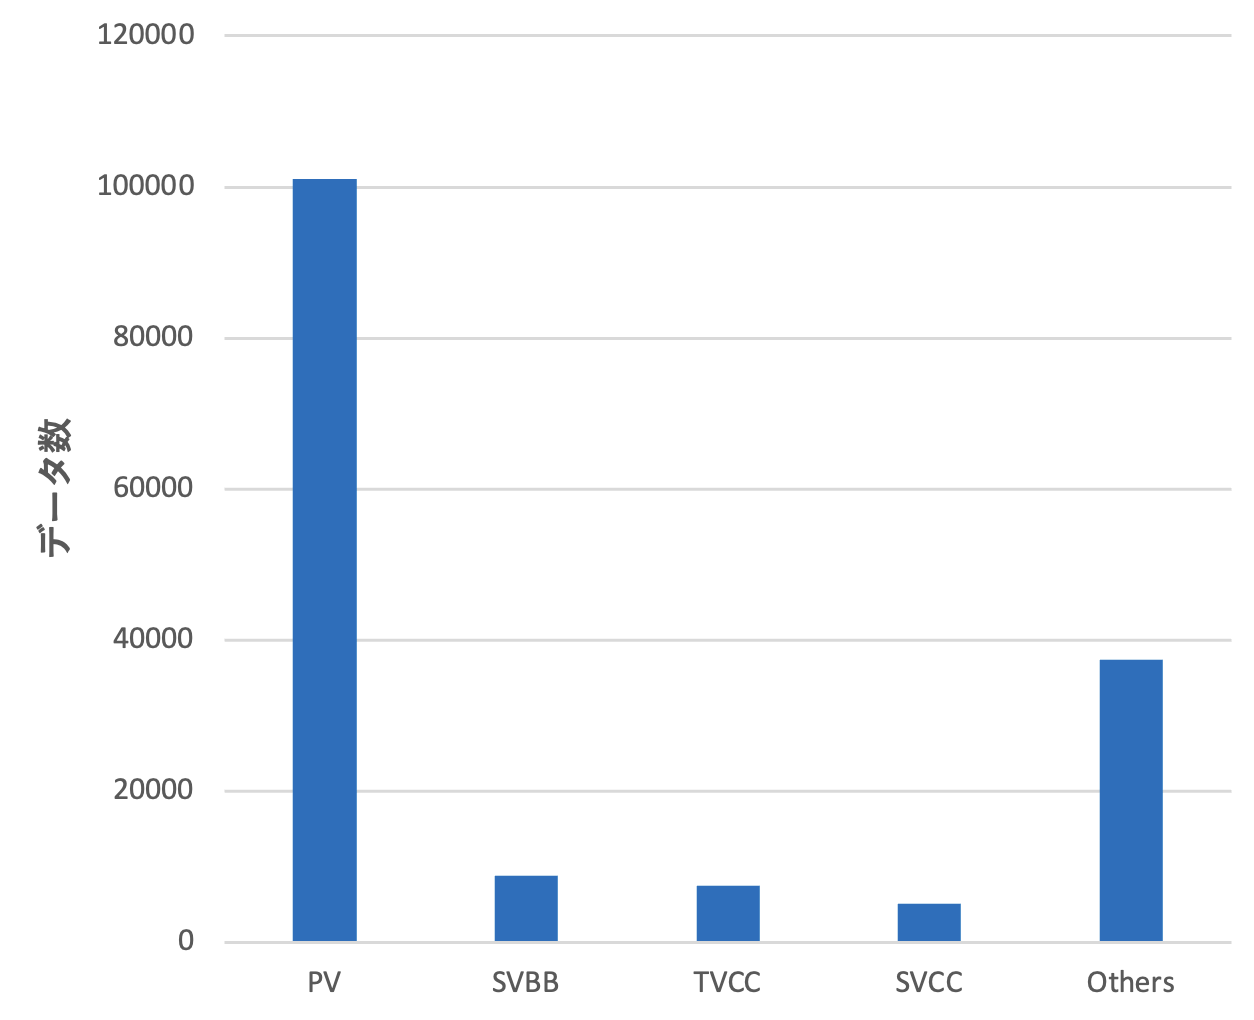
\includegraphics[keepaspectratio, scale=0.5]
 	{Figure/Flavortagging/imbalance.png}
 		\caption{ノードラベル毎のデータ数}
 		\label{node_imb}
	\end{center}
\end{figure}
\subsection{ネットワークアーキテクチャ}
上述の通り、本アルゴリズムではフレーバー識別に加えて、補助学習を導入する。具体的にはノード分類とリンク予測、グラフ分類の3つのタスクを同時に行うネットワークで、図\ref{gnnmodel}のようなモデルを構築した。\\
はじめに、飛跡の変数をより多次元ベクトル化し潜在表現を得るために全結合層を設置する。その後、Graph Attention Network (GAT) を3層設置し、各GAT層の後にはバッチ正規化とReLU関数の活性化関数を置く。そして学習をノード分類、リンク予測、グラフ分類の3つに分岐させる。ノード分類では、飛跡の由来となる崩壊点の種類によって5つの出力が全結合層によって設計されている。リンク予測では、エッジの隣接行列を取得してノード間に隣接があるかないかを判断する2分類問題を行っており、これはエッジが崩壊点となりうるのかの判断に等しい。グラフ分類では、poolingによってグラフ全体の特徴量を1つの次元に置き換え、各フレーバーらしさを出力する設計になっている。\\
GATの学習は\ref{GATexplain}節で述べた通りであり、本アルゴリズムのグラフデータは全結合のグラフニューラルネットワークを構築しており、ノードに対するアテンション$\alpha$はエッジの隣接関係を用いて式\ref{gatattention}のように学習される。このようなアテンション機構によってグラフ全体、すなわちジェットフレーバーの識別を補助することを目的に、ノードの識別の補助学習を導入した。また、実際に飛跡対が崩壊点を共有している場合、その隣接関係は物理的に重要なものとなるため、その情報を学習に活かすことを目的にリンク予測を補助学習に加えた。また、3つの学習の出力層に置いた全結合層はそれぞれ独立に実行される。\\
\begin{figure}[H]
	\begin{center}
 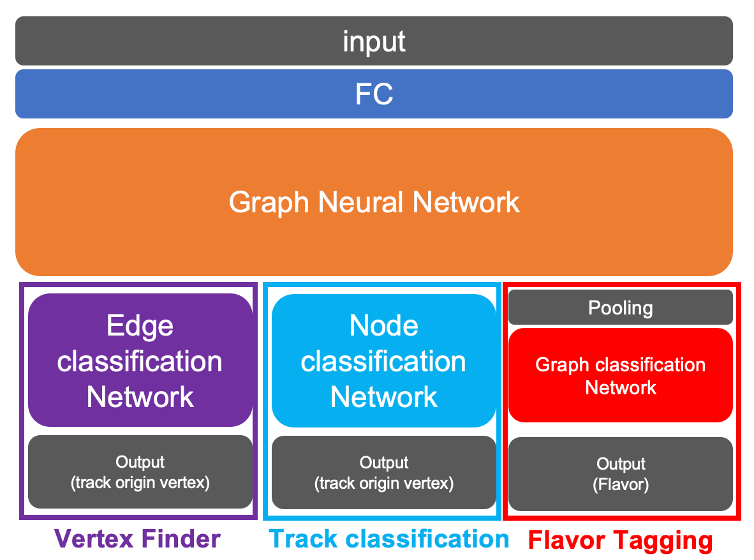
\includegraphics[keepaspectratio, scale=0.4]
 	{Figure/Flavortagging/gnn.png}
 		\caption{フレーバー識別のためのグラフデータを用いたネットワークの概略図}
 		\label{gnnmodel}
	\end{center}
\end{figure}
また本アルゴリズムでは3つの異なる学習を同時に行う必要があり、目的によって相対的な学習のしやすさが異なるため、次のような損失関数をデザインした。\\
\begin{align}
\mathrm{L}_{total} = \mathrm{L}_{graph} + w_{node} \mathrm{L}_{node} + w_{edge} \mathrm{L}_{edge}
\end{align}
$\mathrm{L}$はそれぞれの損失関数を、$w_{node}とw_{edge}$はそれぞれノード、エッジの損失関数にかける重みを表す。グラフ識別と同程度の損失関数に収束するために、ノード識別とリンク予測における損失関数に重み付けを行った。\\
\ また、学習におけるハイパーパラメータにはベイズ最適化を行った上で、表\ref{gnnsetting}に挙げるものを用いた。
\begin{table}[H]
 \centering
  \begin{tabular}{ l  l }
   \hline
   ノード数 & (512, 512, 512)\\
   活性化関数 & ReLU関数\\
   損失関数 & 交差エントロピー\\
   最適化アルゴリズム & RAdam\\
   学習率 & 0.01\\
   Weight decay & 0.0001\\
    $w_{node}$ & 3.0\\
    $w_{edge}$ & 1.0\\
   エポック数 & 100\\
   バッチサイズ & 128\\
   \hline
  \end{tabular}
  \label{gnnsetting}
  \caption{グラフニューラルネットワークにおけるハイパーパラメータ}
\end{table}
\subsection{ハイパーパラメータの最適化}
ネットワークのハイパーパラメータは、ベイズ最適化法によってチューニングを行った。チューニングしたパラメータは表\ref{gnnoptuna}を用いた。チューニングにはディープニューラルネットワークの実装におけるものと同じライブラリを用いたが、評価関数として検証用データの損失関数のうち$ \mathrm{L}_{graph}$のみを用いて、最小になるような最適化を行った。
\begin{table}[H]
\centering
 \begin{tabular}{ l  l }
 \hline
 変数名 & 最適化範囲\\
 \hline
 \hline
 中間層のノード数 & $32 \sim 1024$\\
 アテンションヘッドの数 & $1 \sim 20$\\
 $\alpha$ & $0.0 \sim 5.0$\\
 $\beta$ & $0.0 \sim 5.0$\\
  \hline
 \end{tabular}
 \label{gnnoptuna}
 \caption{最適化を行ったハイパーパラメータとその値の範囲。}
\end{table}
\subsection{学習評価}
はじめに、学習全体の結果を図\ref{gnnoutput}に示す。学習の経過を通して損失関数は減少しており、特に80epoch付近で急激な降下を見せた。しかしそれ以降は過学習が進んでしまい、損失関数の値は安定化させることが難しかった。また、ノード、リンク、グラフそれぞれの精度においても、学習の経過を通して向上が見られた。\\
\begin{figure}[H]
	\begin{center}
 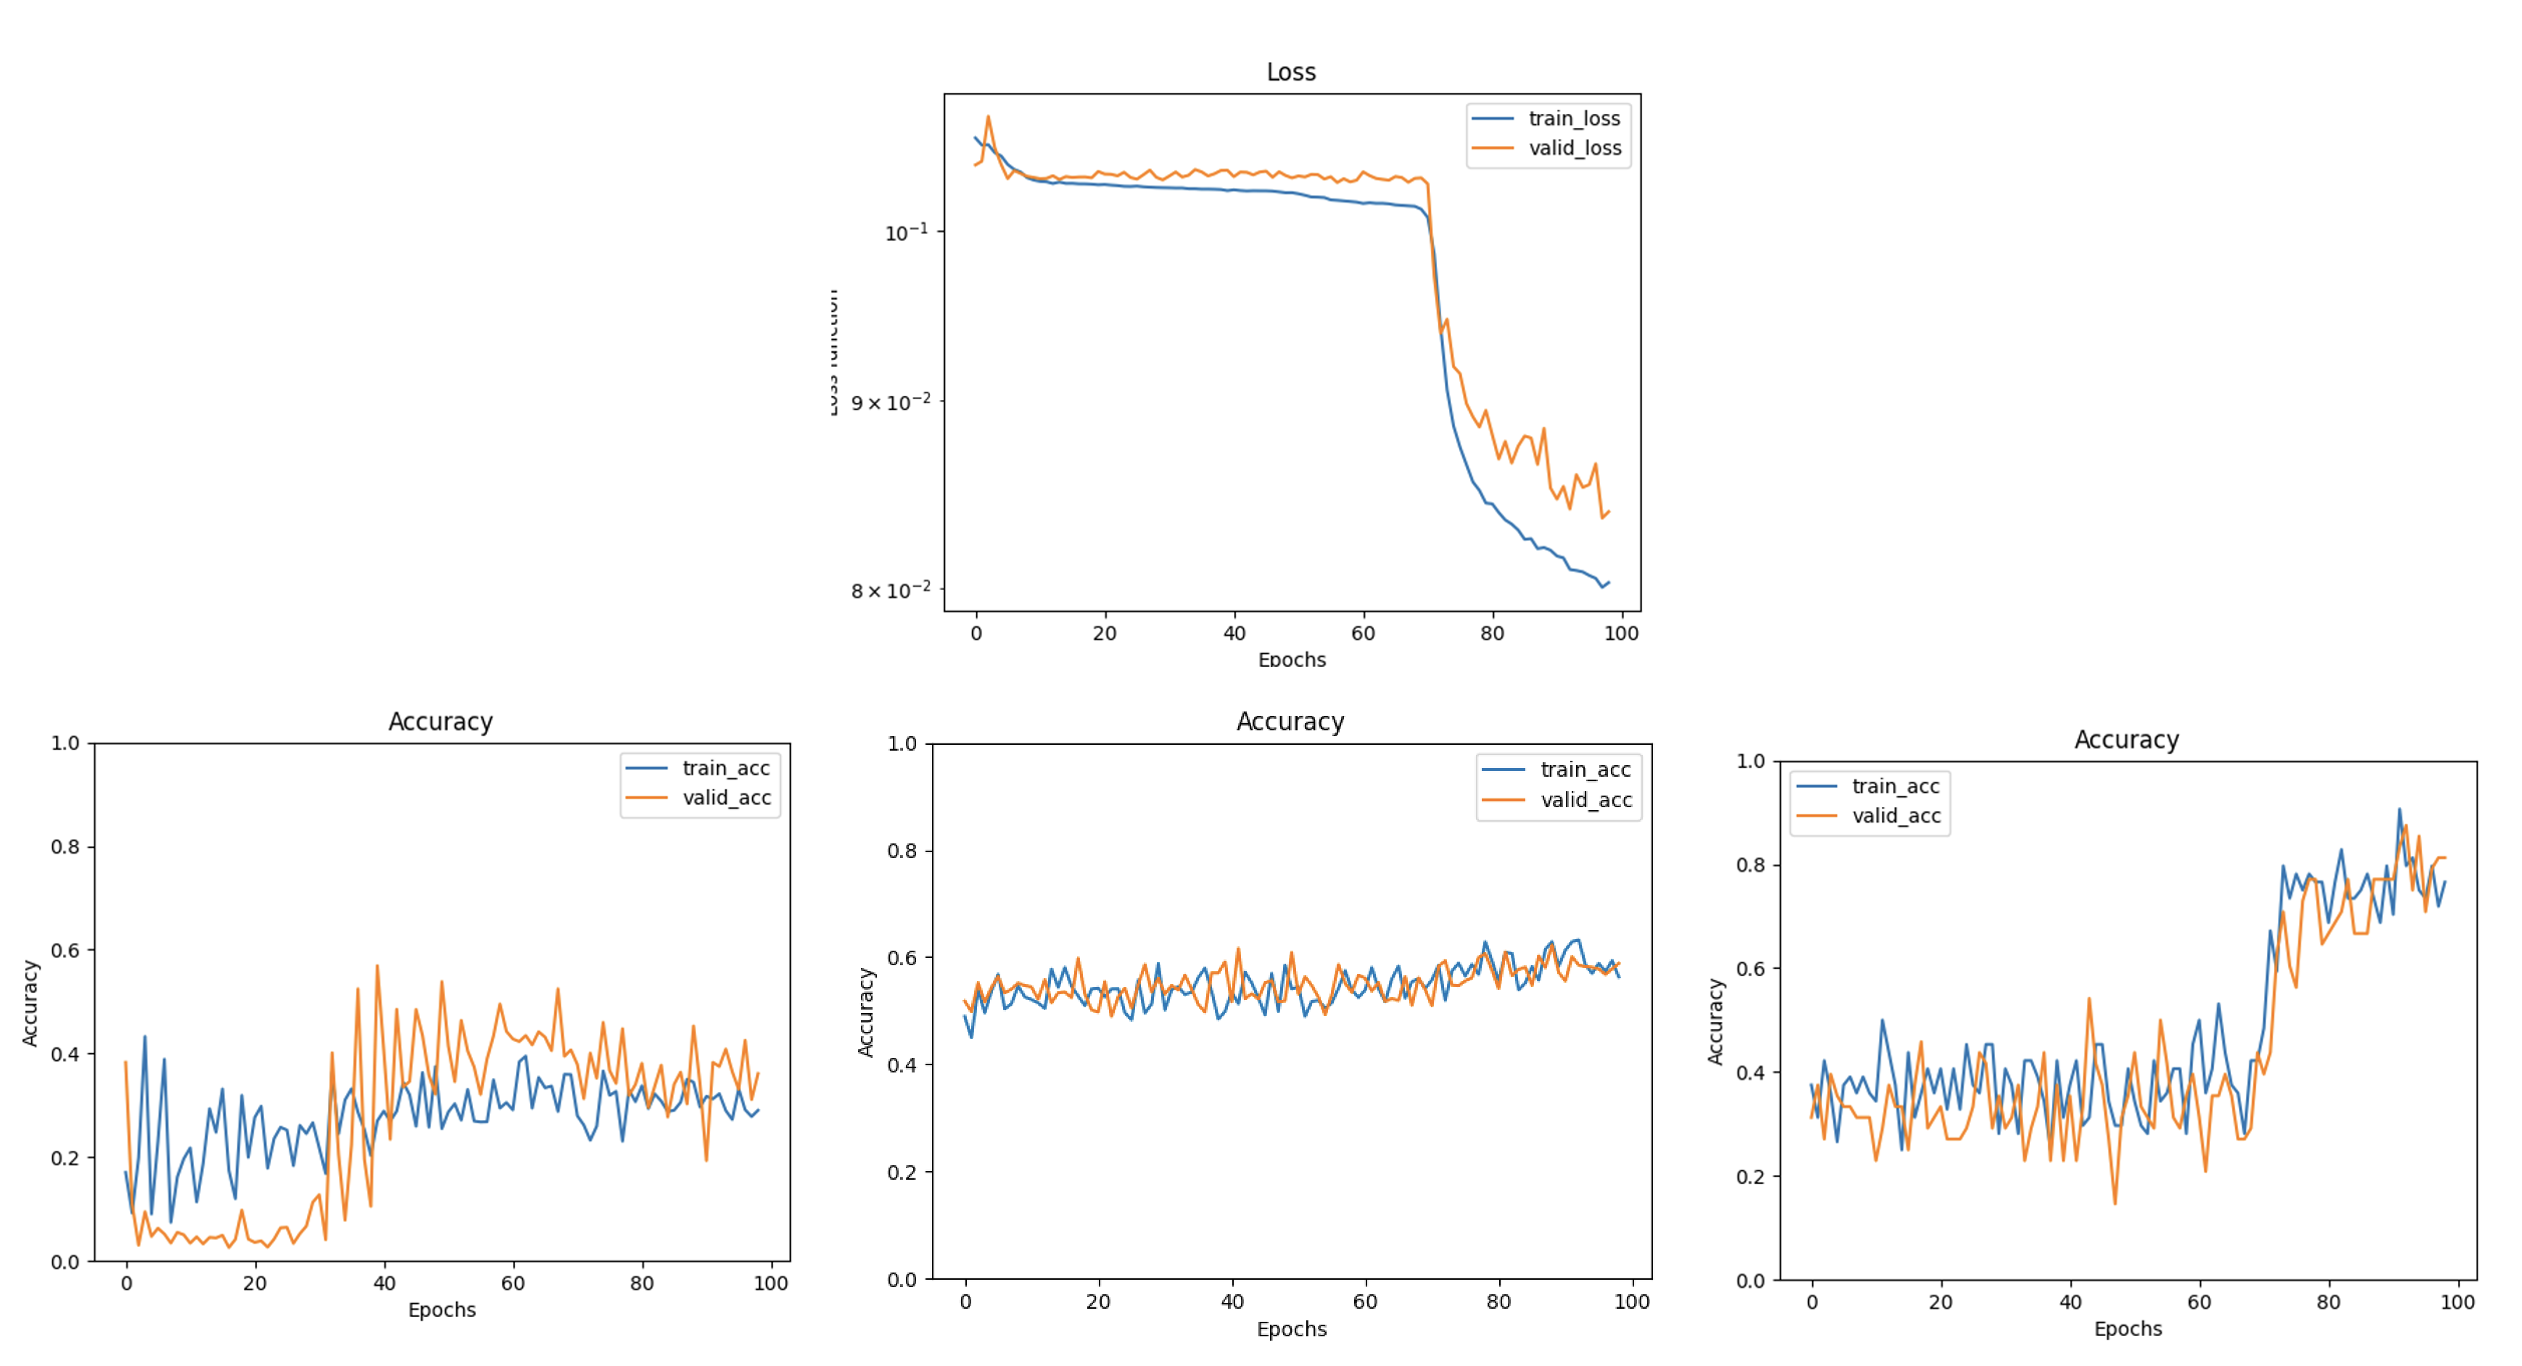
\includegraphics[keepaspectratio, scale=0.3]
 	{Figure/Flavortagging/gnnoutput.png}
 		\caption{(上)学習の経過における損失関数。(左下) 学習の経過におけるノードの学習精度、(中央下) リンクの学習精度、(右下) グラフの学習精度。}
 		\label{gnnoutput}
	\end{center}
\end{figure}
続いて、ノード、リンク、グラフ識別における混合行列を図\ref{gnncm}に示す。ノード、リンクの学習精度は十分良いと言える制度ではなく、一方でグラフの識別においてはディープニューラルネットワークでの実装に匹敵する精度が得られた。ノードの混合行列ではPVとSVBBと識別する割合が高く、一方でTVCC、Othersについて分類が出来ずPVに分類されてしまう傾向にあった。\\
\begin{figure}[H]
	\begin{center}
 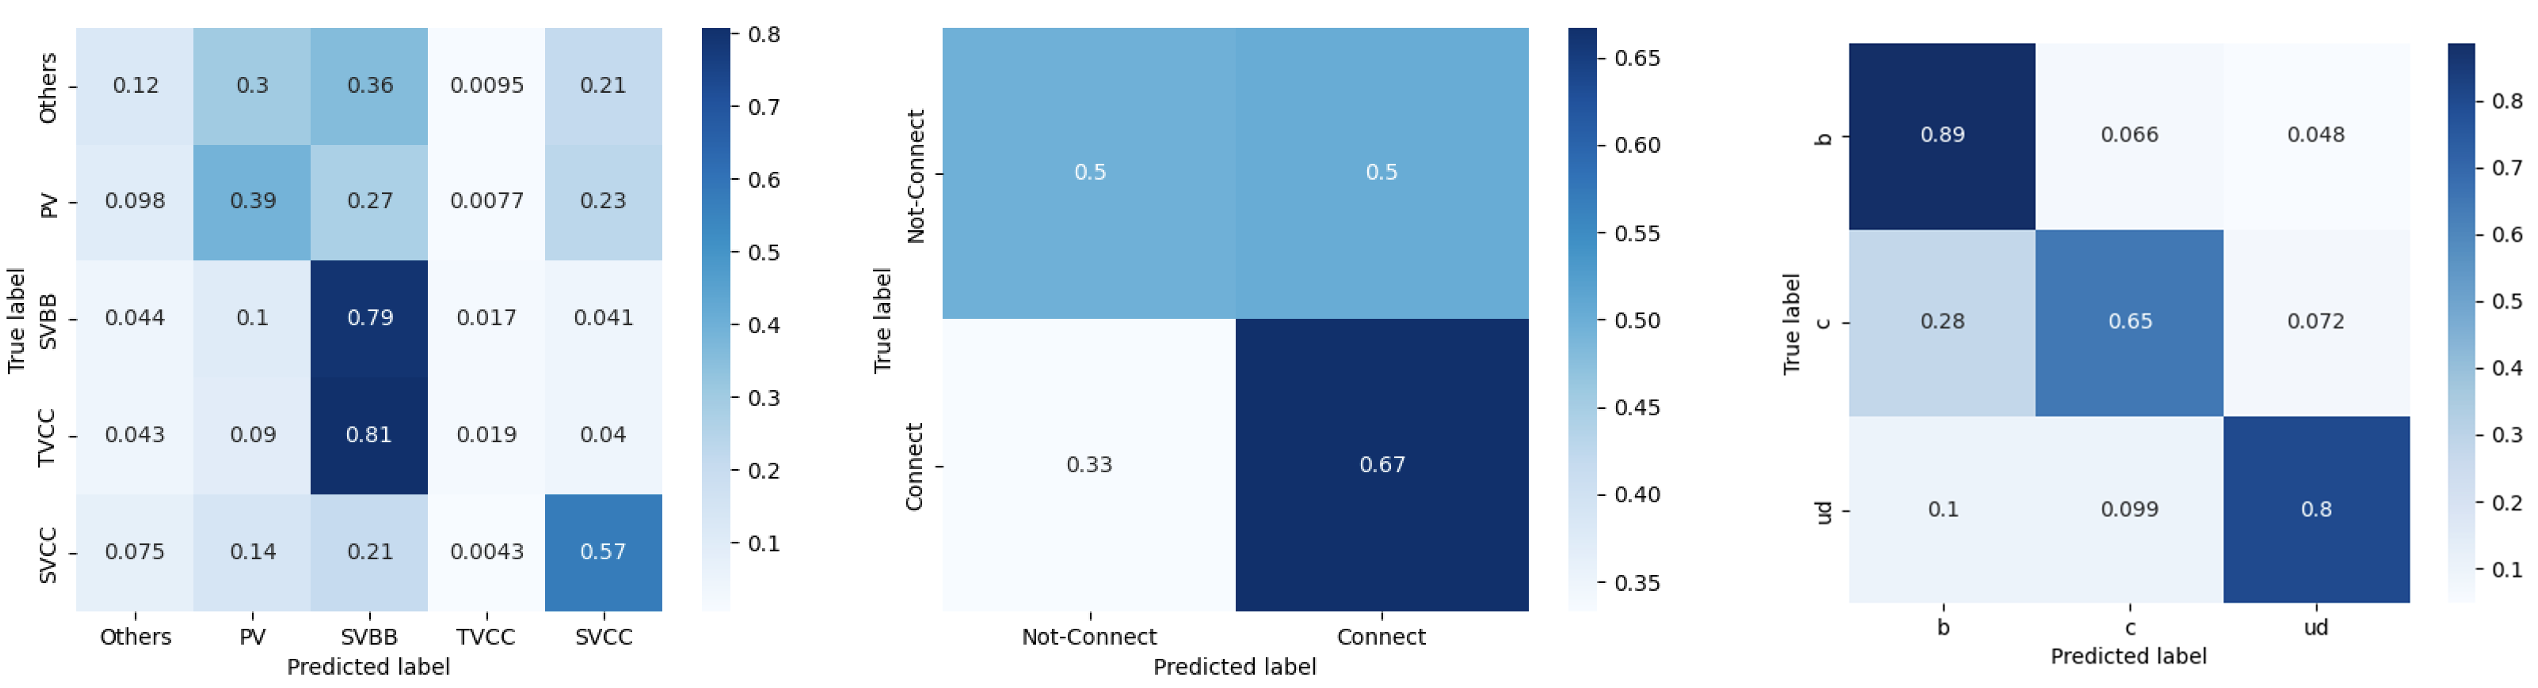
\includegraphics[keepaspectratio, scale=0.3]
 	{Figure/Flavortagging/gnncm.png}
 		\caption{(左) ノード分類の混合行列、(中央) リンク予測の混合行列、(右) グラフ識別の混合行列。}
 		\label{gnncm}
	\end{center}
\end{figure}
最後に、LCFIPlusとの比較を示す。ディープニューラルネットワークの比較と同様に、図\ref{gnneff_b}, \ref{gnneff_c} は b/c ジェットの識別効率のプロットを
%、表\ref{gnn_lcfi}は識別効率を 80\% (Tagging Efficiency = 0.8) に固定したときの背景ラベルの識別効率の 割合を
示している。bジェットの識別効率はcジェットについて向上しており、識別効率80\%における識別割合は、LCFIPlus が c ジェットの識別割合が 7.3\%、uds ジェットの識別効率が 0.74\% であるのに対して、グラフニューラルネットワークのcジェットの識別割合はおよそ1.5\%、udfジェットの識別効率もおよそ1\%ほどという結果になり、cジェットの誤認率が5分の1程度になっているものの、udsジェットに関しては若干の精度低下となった。また、cジェットの識別効率は非常に悪い結果となってしまい、識別効率80\%における識別割合は、LCFIPlus がbジェットの識別割合が 22\%、udsジェットの識別効率が 24\% であるのに対して、グラフニューラルネットワークのbジェットの識別割合はおよそ40\%、udfジェットの識別効率はおよそ15\%ほどという結果になり、bジェットの誤認率が2倍近く上がってしまった。ノード分類結果では、PVとSVBBと識別する割合が高いことから、bジェットに対する識別効率が高くなっていることが考えられる。また、cジェットのbジェットとの分離が悪い点に関しては、主にSVBB,TVCCに対するSVCCの分類精度が課題となっていると推測される。\\
\begin{figure}[H]
	\begin{center}
 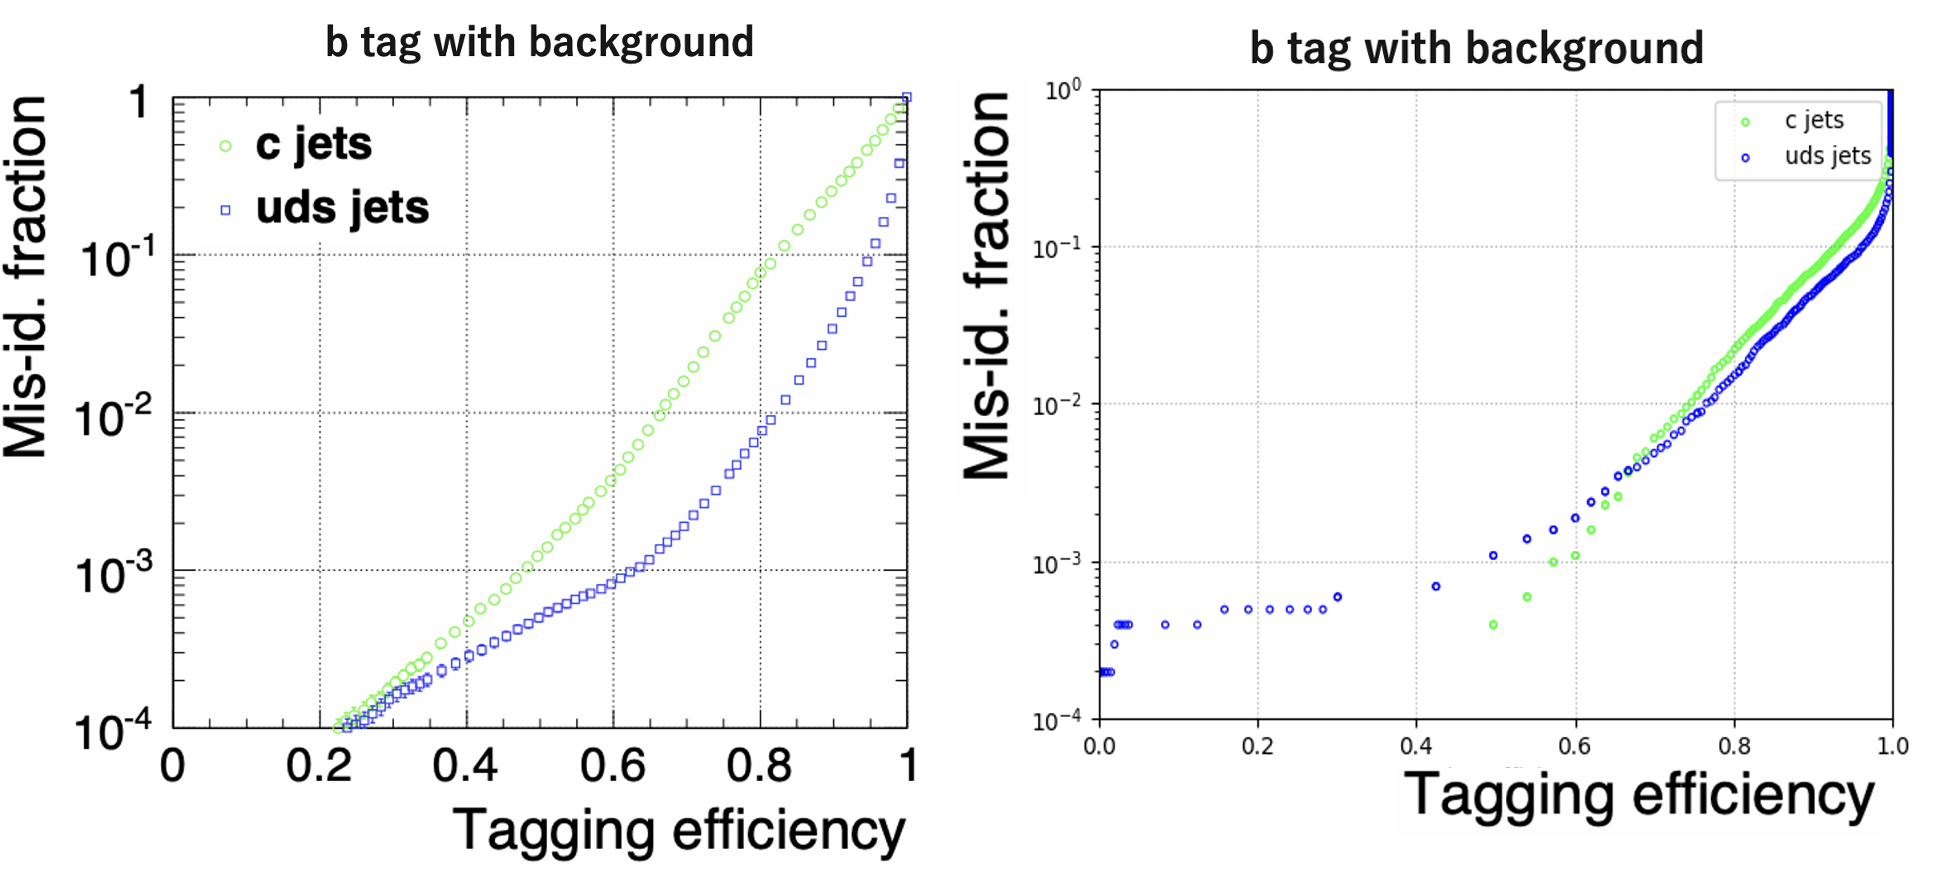
\includegraphics[keepaspectratio, scale=0.3]
 	{Figure/Flavortagging/gnneff_b.png}
 		\caption{LCFIPlus(左)とグラフニューラルネットワーク(右)によるbフレーバージェットの識別効率の比較。緑:bジェットに対するcジェットの識別効率、青:bジェットに対するudsジェットの識別効率を示している。}
 		\label{gnneff_b}
	\end{center}
\end{figure}

\begin{figure}[H]
	\begin{center}
 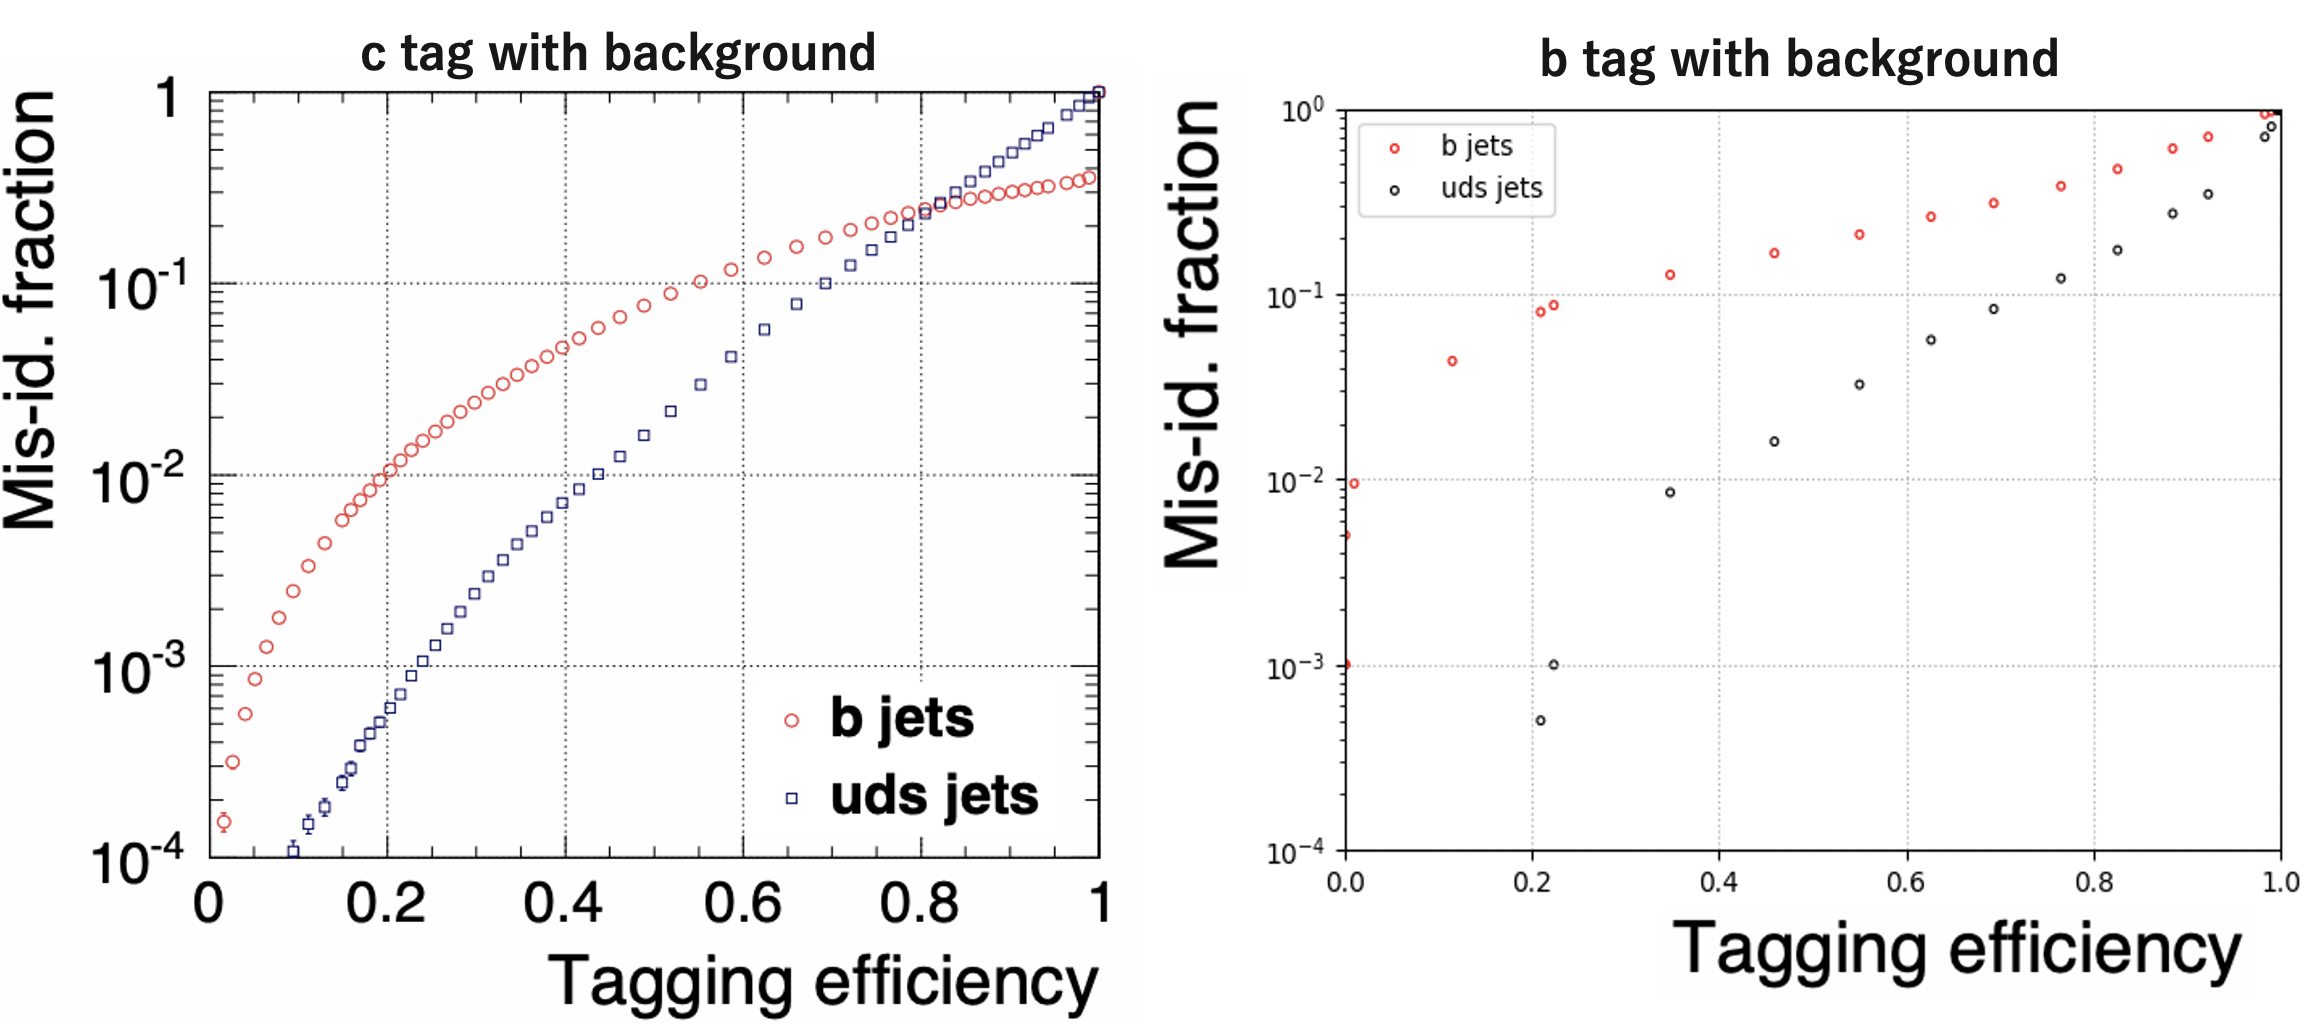
\includegraphics[keepaspectratio, scale=0.3]
 	{Figure/Flavortagging/gnneff_c.png}
 		\caption{LCFIPlus(左)とグラフニューラルネットワーク(右)によるcフレーバージェットの識別効率の比較。赤:cジェットに対するbジェットの識別効率、黒:cジェットに対するudsジェットの識別効率。}
 		\label{gnneff_c}
	\end{center}
\end{figure}

\begin{comment}
\begin{table}[H]
 \centering
  \begin{tabular}{ |c|c|c|c|}
   \hline
   \multirow{2}{c}{識別効率=0.8} & \multirow{2}{c}{背景ジェット} & \multicolumn{2}{|c|}{誤認率} \\
    & & LCFIPlus & GNN\\ \cline{3-4} 
    \hline \hline
   \multirow{2}{c}{bジェット} & cジェット & 0.073 & $\sim$ 0.015\\ \cline{2-2} 
   & udsジェット & 0.0074 & $\sim$ 0.01 \\ \cline{1-2} 
   \multirow{2}{c}{cジェット} & bジェット & 0.22 & $\sim$ 0.40\\ \cline{2-2} 
   & udsジェット & 0.24 & $\sim$ 0.15\\
   \hline
  \end{tabular}
  \caption{識別効率 (Tagging Efficiency) に対するジェット誤認率 (Mis-id fraction)}
  \label{gnn_lcfi}
\end{table}
\end{comment}
結果として、グラフニューラルネットワークによる実装ではLCFIPlusと比較して顕著な性能向上があったとは言えない結果になった。しかしながらエッジリンク予測の実行によって、これまで別のプロセスで実行していた崩壊点検出を、1つのネットワーク内で内包することが出来た。
 % !TEX root = ../MasterThesis_Onoe.tex
% 上記はただのコメントではなく親ファイルの場所を教えているので
% 消してしまうとファイルごとのタイプセットができなくなるので注意。
% 親ファイル名を変更したときはここも変更する。

\chapter{まとめと今後の展望} \label{sec:Conclusion}
本論文では、電子陽電子ヒッグスファクトリーのためのジェット測定技術の研究として、特にILCを念頭に置いた2つのテーマの研究を行った。1つ目のテーマでは、ILCの検出器案であるILDの電磁カロリメータのうち、SiW-ECALの技術プロトタイプを高エネルギービーム試験によって性能評価した。2つ目のテーマでは、深層学習を用いたフレーバー識別アルゴリズムの開発を行った。本章ではそれぞれの研究のまとめと今後の展望について述べる。

\subsection*{ILD SiW-ECAL プロトタイプの高エネルギービーム試験による性能評価}
本研究では、ILD SiW-ECAL プロトタイプの高エネルギービーム試験による性能評価を行った。ILDはILCの検出器の候補であり、PFAに最適化された構造となっている。ILDを構成するECALには高精細なカロリメータが求められており、その候補としてSiW-ECALがある。SiW-ECALは$\SI{5.5}{mm} \times \SI{5.5}{mm}$のピクセルシリコンセンサーを読み出しに用いた高精細なカロリメータであり、CALICEコラボレーションによって技術プロトタイプが開発されている。本研究では、CERN SPS加速器における$10 \sim \SI{200}{GeV}$高エネルギービームを用いてプロトタイプの性能評価実験を行った。実験後の解析では、大きく3つの課題点が見つかった。1つ目はセンサーが一部剥がれてしまい、全てのチャンネルでデータの取得ができなかった点である。これは運搬中の衝撃や経年劣化によるボードの変形によってセンサーが剥がれてしまったと予想いる。また2つ目は$\SI{80}{GeV}$以上の高エネルギービームをSiW-ECALに照射すると、一部のセンサーではセンサー全体に本来のヒットとは異なるトリガーが収集されてしまった点である。これはエネルギーが高くなった際にセンサー周辺で放電現象等が起きていることなどが原因として推察されるが、現在も引き続き調査を行なっている。また、2つ目は複数の読み出しチャンネルにおいて、ペデスタルのピークが2つ (ダブルぺデスタルと呼ぶ) 確認された点である。これはヒットによる信号を求める上で大きな問題となり、この現象についてその発生箇所やピークの振る舞い等の調査を行なった。解析の結果、ダブルぺデスタルは内部配線や外部接続をアップデートする以前のFEV10、11に多く発生しており、また発生箇所も多くはボードの電源部に近いところで発生していた。そのため、ダブルぺデスタルは電源に由来する現象であることが推測することができる。今後の方針として、センサー剥がれについては、センサーとボードの接着の見直しをおこない、また同様の現象が起こらぬよう耐久性の試験や劣化を抑える保存方法の検討が挙げられる。また、ダブルぺデスタル現象に対しては、ダブルぺデスタルを引き起こしている配線を特定することで次世代のアップデートに向けた施策を練ることや、その発生条件についてより詳細な解析を行い信号の選択によって取り除くことを目指すことが考えられる。

\subsection*{深層学習を用いたフレーバー識別アルゴリズム}
本研究では、深層学習を用いたフレーバー識別アルゴリズムの開発を行った。ヒッグスファクトリーの目的であるヒッグス粒子は、クォークやグルーオンなどに崩壊し、多数のハドロンの束であるジェットとして検出器に到達する。そのためジェットの再構成でクォークのフレーバーを識別することは、ヒッグスの物理を知るための解析において非常に重要な情報となる。フレーバー識別はジェットの構成粒子の種類や運動量、崩壊点に関する情報から、ジェットの元となるクォークのフレーバーを識別するプロセスであり、現在ジェットの再構成に用いられているLCFIPlusでは従来の機械学習手法であるBDTsが用いられている。これに対して深層学習を導入することで、識別性能の向上や崩壊点検出アルゴリズムとの統合などを目指した。

はじめに、最も単純な構造のネットワークモデルであるディープニューラルネットワークによる実装を行った。アルゴリズムには過学習対策や学習の効率化に向けた手法を用いて、全結合層を中心としたディープニューラルネットワークのモデルを、PyTorchを用いて構築した。学習の入力データとして、$\SI{250}{GeV}$のILDフルシミュレーションのイベント400万イベントを、変数にはBDTsの学習に用いた変数と同じものを用いた。学習を重ねるにつれて損失は減少し、学習全体の精度はおよそ82.5\%で得られた。またLCFIPlusとの比較にあたっては、識別効率あたりの誤認率によって比較した。結果として、$c$ジェットの識別など一部で改善が見られたものの、LCFIPlusと大差ない、あるいはやや劣る結果となった。

続いて、グラフデータを用いたフレーバー識別アルゴリズムの実装を行った。動機としては、フレーバー識別において重要なIP付近の物理現象をグラフ構造のデータとして構築することで、物理量を羅列する1次元の数値データと比較して表現力が上がり、性能が向上するのではないかという狙いがあった。またグラフデータを構築する際の副産物として、以前は別プロセスであった崩壊点検出を1回の識別で同時に処理できるという長所もあった。グラフデータは独自のデータセットクラスを作成し、飛跡をノードとする全結合のグラフを、1ジェットあたり1グラフ構築した。また、このグラフではディープニューラルネットワークと異なり、ノードのみ飛跡再構成におけるフィッティングパラメータを特徴量を持つとした。イベントは$\SI{250}{GeV}$のILDフルシミュレーションのイベント240万イベントを用いた。ネットワークアルゴリズムはGATを3層使用し、損失関数の工夫やデータ次元変更などの手法を用いてノード識別/リンク予測/グラフ分類の3つのタスクを同時に実行し、重みを共有するようなネットワークモデルをPyTorch Geometricを用いて実装した。学習は不安定であったものの損失は減少し、ディープニューラルネットワークに匹敵するグラフ分類の精度が得られた。また識別効率あたりの誤認率のプロットによるLCFIPlusとの比較では、$b$ジェット識別において改善が見られたが、$c$ジェット識別では非常に悪い結果となった。またノード識別、リンク予測に対しては十分に良い精度を得ることができなかった。しかし、低い精度ながら崩壊点検出アルゴリズムの統合を達成することができた。

今後の展望として、フレーバー識別アルゴリズムには大きく2つの方向性で改善が可能であると考えている。

1つ目は深層学習の理論・技術面での方向性である。GATに挙げられるネットワークの処理に関してより理解を深め、フレーバー識別により最適なネットワーク構造を提案することや、物理的な性質をより組み込むなどフレーバー識別に最適化された損失関数を設計するなど、演算手法によって更なる改善の見込みがあると考えている。また、グラフデータの設計についても改善ができると考えており、具体例としては今回のデータセットにおいて崩壊点となるエッジに特徴量を持たせることや、グラフデータの構成要素を変更することなどが挙げられる。現在エッジは特徴量を持っておらず、接続したノードの情報のみで更新を行っているが、エッジ自身が特徴量を持つことでデータの学習パラメータが増え、精度が向上すると考えることができる。また、本研究では飛跡をノードとするグラフを構成したが、本来飛跡は点ではなく曲線の形状を取るため、やはり崩壊点のような物理的に点となる量をノードとすることで、実際の物理現象に近いグラフの構築が期待できると考えている。

2つ目は、iLCSoftとしての実装に向けた方向性である。例えば出力情報の設計やC++環境への移行があると考えている。出力設計に関して、今回のグラフデータを用いたフレーバー識別では崩壊点検出を包含するアルゴリズムを開発した。しかし、現段階では解析において崩壊点の情報が必要になった際、物理量として出力することは出来ない。そのため方針としては、中間層で得たネットワークの潜在的なパラメータを回帰問題として設計することで、新しく崩壊点など数値データの出力を得ることなどが考えられる。また別の例としては、開発したフレーバー識別アルゴリズムのC++環境への移植である。現在ジェット再構成に用いられているLCFIPlusはMarlinプロセッサーの1部であり、C++環境で動作している一方で、本研究で開発したアルゴリズムはpythonによって記述されている。そのためPyTorch/PyTorch Geometrc C++ APIを用いる、あるいはC++によって書き換えを行うことによるiLCSoftへの実装は、今後の課題の一つである。
\fi

%----------------------------------------------------------------------------------------------------
%----- 付録
\ifabstract\else
 \appendix
 % !TEX root = ../MasterThesis_Onoe.tex
% 上記はただのコメントではなく親ファイルの場所を教えているので
% 消してしまうとファイルごとのタイプセットができなくなるので注意。
% 親ファイル名を変更したときはここも変更する。

\appendix 

\chapter{AppendixA} \label{sec:Appendix}
\section{飛跡のパラメータ}
\subsection{LDC座標系}
ILCにおいて検出器を通過する荷電粒子には、飛跡を記述する際に専用の手法が用いられており、それによってシミュレーションツールなどで変換を行うことなく、データを解析することができる。この手法はILDの母体となったLarge Detector Concept (LDC) よって定義された座標系\cite{ldc}を基に定義されており、LDC座標系は次のように定義される。
\begin{enumerate}
\item 右手系直交座標。
\item 電子陽電子の相互作用点を原点とする。
\item ビーム方向に沿ってz軸をとる。
\item 垂直上方向にy軸をとる。
\end{enumerate}

この座標系における任意のベクトル$\bm{v}$は球面座標系において、次のように表される。

\begin{align}
\mathbf{v} &= \left(
\begin{array}{c}
|\mathbf{v}| \sin \theta \cos \phi \\
|\mathbf{v}| \sin \theta \sin \phi \\
|\mathbf{v}| \cos \theta \\
\end{array}
\right) \\
\nonumber \theta& \in [0,\pi ] \\
\nonumber \phi &\in [-\pi , \pi ]
\end{align}

\subsection{飛跡パラメータ}
ILCで発生する荷電粒子は一定の磁場の影響を受け、螺旋軌道を描く。磁場はz軸に並行な方向に一様にかかるものとする。この時、荷電粒子の飛跡は$xy$平面への射影における円となり、z軸方向の変位は弧の長さsの線形関数となる。

荷電粒子は運動の基準点$\mathbf{P}^r = \left( P_x^r, P_y^r, P_z^r \right)$と飛跡パラメータ$\left( \Omega, {\phi}_0, d_0, z_0, \tan \lambda \right)$によって定義される。また、以下の定義において$\mathbf{P}^0$は$xy$平面上の基準点への最近接点を表す。
\subsubsection{$xy$平面}
$xy$平面( 図\ref{xy} )では荷電粒子の移動は、以下のように定義される。\cite{lcio}
\begin{itemize}
\item ${\phi}_0$は運動量の$P_0$における方位角を表す。\\
\item $\Omega$は飛跡の曲率を表す。\\
\begin{align}
|\Omega | = \frac{1}{R}
\end{align}
ここで、Rは飛跡の曲率半径を表す。\\
\item $d_0$は$xy$平面のインパクトパラメータを表す。$\mathbf{d} = (d_x, d_y)$を任意の点$\mathbf{P}^r$から$\mathbf{P}^0$までのベクトルとする。\\
\begin{align}
\mathbf{d} = \mathbf{P}^0 - \mathbf{P}^r
\end{align}
また、$\mathbf{P}^0$から飛跡への法線ベクトルを$\mathbf{n}_{pca}$とすると、$d_0$は以下のように表される。
\begin{align}
d_0 = \mathbf{n}_{pca} \cdot \mathbf{d} = - ( P_x^r - P_x^0 ) \sin {\phi}_0 +  ( P_y^r - P_y^0 ) \cos {\phi}_0
\end{align}
$|\mathbf{n}_{pca}|$であるため、$|d_0|$は$xy$平面における$\mathbf{P}^r$と$\mathbf{P}^0$の距離を表す。
\end{itemize}
$xy$平面における円の中心点$\mathbf{P}^c$は、通常$\mathbf{P}^r$と異なる点を取ることが多く、軌道上の任意の点における運動量を$\mathbf{P} = \left( P_x, P_y, P_z \right)$とすると、$\mathbf{P}^c$は以下のように計算される。
\begin{align}
P_x^c &= P_x + \frac{\sin \phi}{\Omega}\\
P_y^c &= P_y + \frac{\cos \phi}{\Omega}\\
\end{align}
\begin{figure}[H]
	\begin{center}
 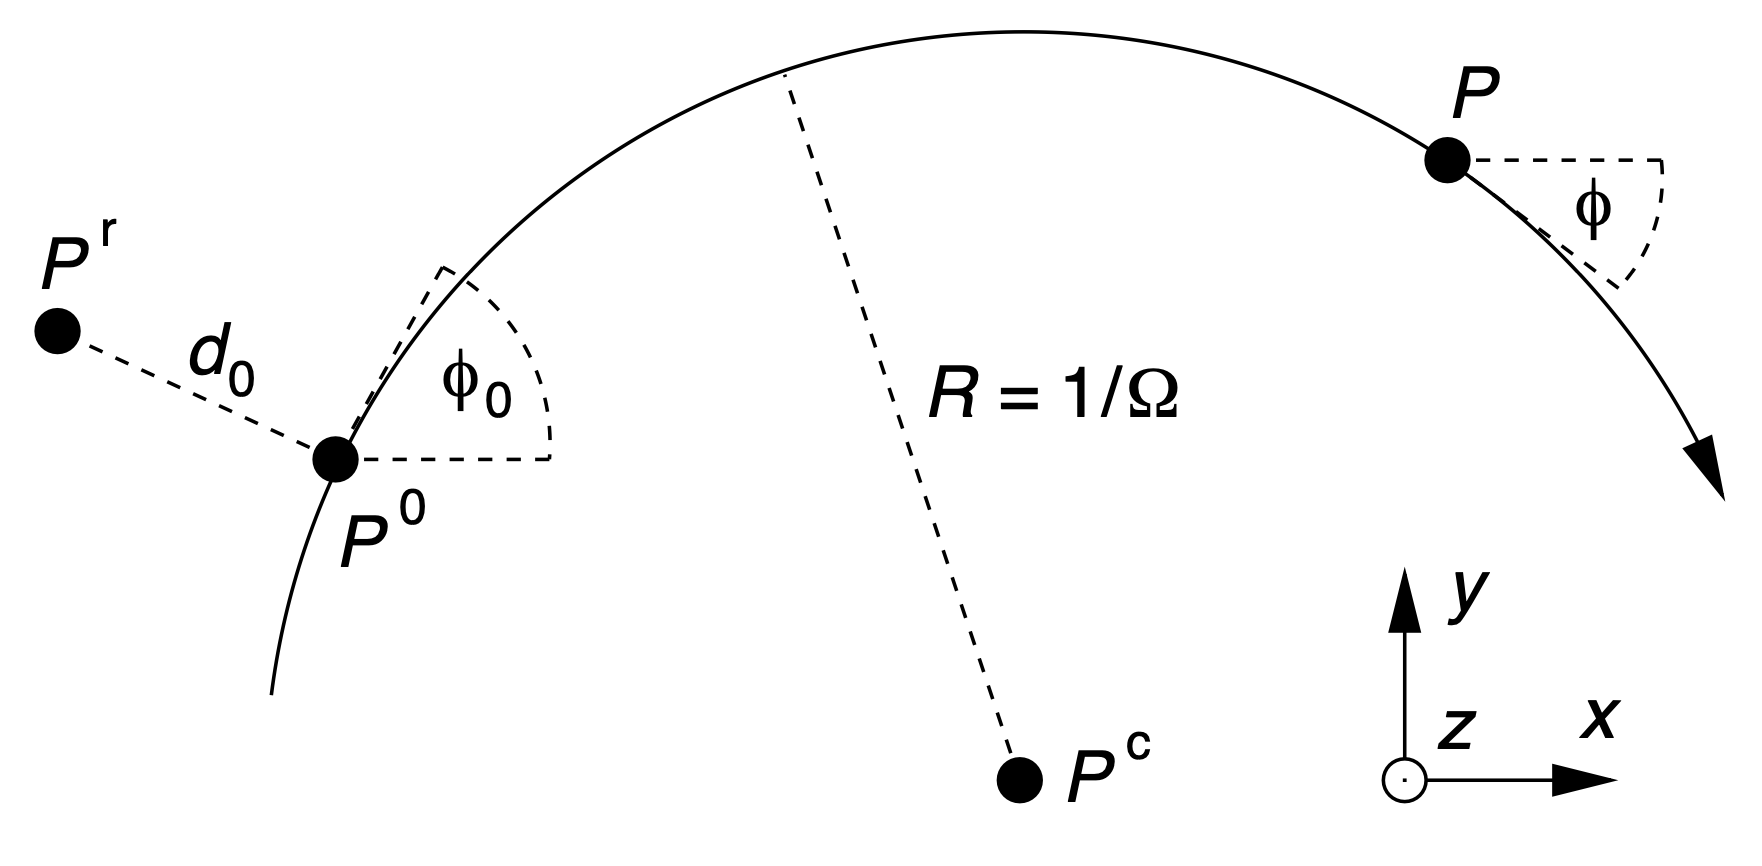
\includegraphics[keepaspectratio, scale=0.4]
 	{Figure/Appendix/xy.png}
 		\caption[飛跡の$xy$平面への射影]{飛跡の螺旋軌道を$xy$平面へ射影した図。軌道は中心点$\mathbf{P}^c$、半径Rをもつ円弧で表される。また、全ての飛跡パラメータは基準点$\mathbf{P}^r$を中心に与えられる。}
 		\label{xy}
	\end{center}
\end{figure}

\subsubsection{$sz$平面}
$sz$平面( 図\ref{sz} )において、飛跡は直線に沿って移動し、2つのパラメータ$(\tan \lambda, z_0)$によって表される。
\begin{itemize}
\item $\tan \lambda$は$sz$平面における直線の傾き$dz/ds$を表し、運動量ベクトル $\mathbf{p} = \left( p_x, p_y, p_z \right)$に対して以下のように計算される。
\begin{align}
\tan \lambda =\frac{p_z}{\sqrt{p_x^2 + p_y^2}} = \cot \theta
\end{align}
\item $z_0$は基準点$\mathbf{P}^r$から$\mathbf{P}^0$までのz軸上の距離を表す。\\
\begin{align}
z_0 = P_z^0 - P_z^r
\end{align}
\end{itemize}
これらを踏まえ、飛跡の$sz$平面射影の軌跡zは、$xy$平面における飛跡の経路積分sを用いて次のように表される。
\begin{align}
z = ( z_0 + P_z^r) + s \cdot \tan \lambda
\end{align}
\begin{figure}[H]
	\begin{center}
 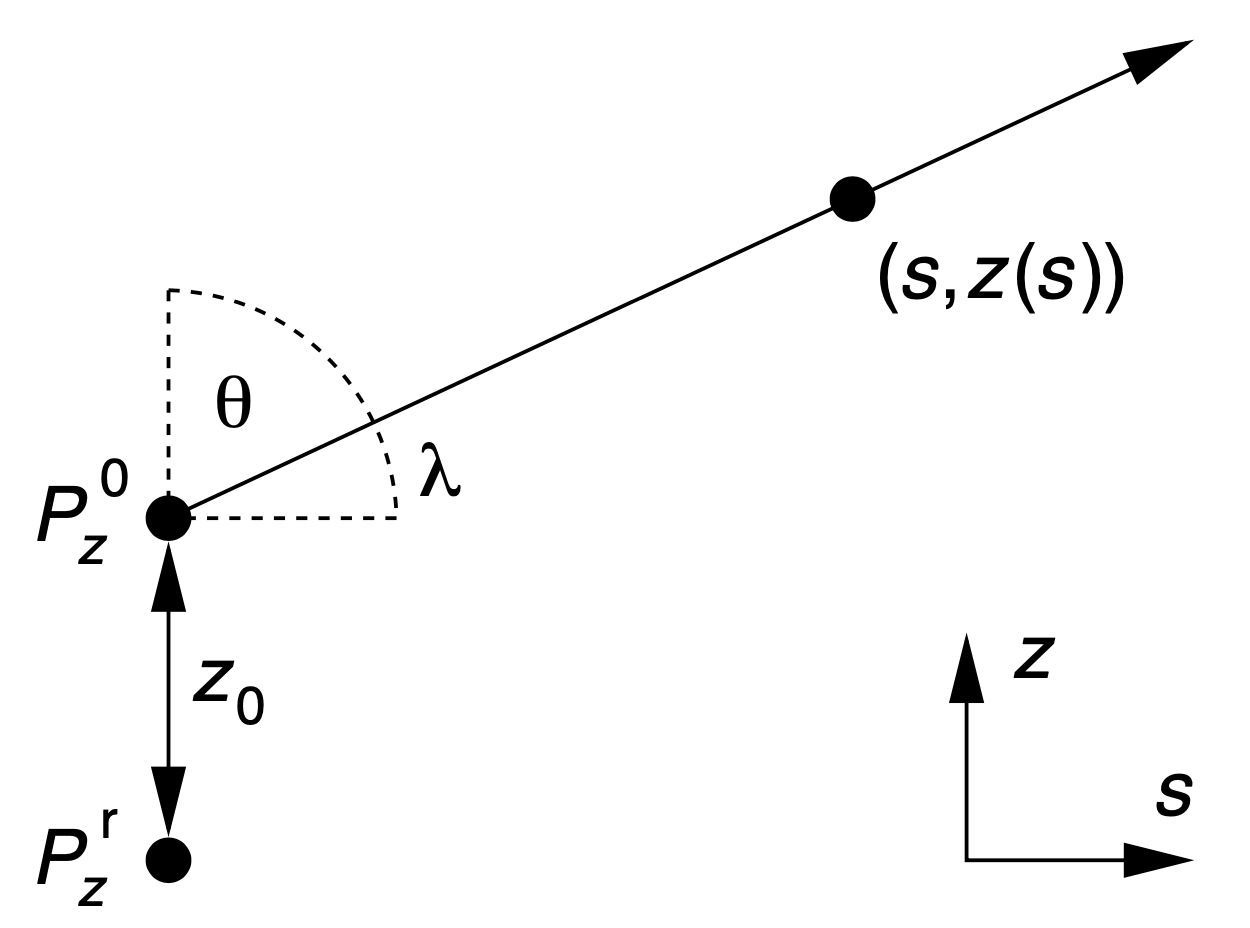
\includegraphics[keepaspectratio, scale=0.4]
 	{Figure/Appendix/sz.png}
 		\caption{飛跡のsz平面への射影}
 		\label{sz}
	\end{center}
\end{figure}

\fi

%----------------------------------------------------------------------------------------------------
%----- 謝辞
\ifabstract\else
 % !TEX root = ../MasterThesis_Onoe.tex
% 上記はただのコメントではなく親ファイルの場所を教えているので
% 消してしまうとファイルごとのタイプセットができなくなるので注意。
% 親ファイル名を変更したときはここも変更する。

\clearpage

\chapter*{謝辞} \label{sec:Acknowledgement}
本研究を進めるにあたり、お世話になりましたすべての方々に感謝申し上げます。

本研究テーマは、指導教員である末原大幹助教に授けて頂きました。末原助教は、日々の研究において私の理解に寄り添い、多くの的確な助言を与えて下さいました。また、国内外での高エネルギー加速器実験への参加や学会・国際会議での発表など、新しいことに挑戦する機会もたくさん与えて頂きました。お陰様で貴重な経験を積み重ね、多くを学ぶことが出来ました。心より感謝致します。川越清以教授には、ゼミナールを通して素粒子物理学の基礎からILCに至るまで、素粒子実験の基礎を教えていただきました。また、研究の進捗報告や学会の発表練習においても多くの助言を頂き、本論文の執筆においても細かにご指導していただきました。厚くお礼申し上げます。
東城順治教授には学部4年次の素粒子物理学の講義において、素粒子物理の基礎を教えて頂きました。吉岡瑞樹准教授には、学部3年次のプログラミングの講義を通してプログラミングによる数値計算の基礎を教えて頂きました。森津学助教には3年生実験のTA業務や、高校生の体験授業において大変お世話になり、親身になってご相談に乗って頂きました。音野瑛俊助教には、CERNにて最先端の実験施設や研究について教えて頂き、その他の面でもサポート頂きました。山中隆志助教には TA 業務で助言をいただいたほか、 g-2実験のASIC検査業務では普段の研究では出来ない経験をさせて頂きました。小林大元特任助教、細川律也学術研究員、小川真治特別研究員、水野貴裕学術研究員にはゼミナールや論文紹介の際に的確なご指摘やご指導を頂いたほか、研究室生活においても色々な話をする機会があり楽しく研究生活を過ごせました。テクニカルスタッフの重松さおり氏には、出張や研究室内の物品管理など研究に関わる事務作業において大変お世話になり、集中して研究に取り組むことが出来ました。また、理学部等事務部や物理学事務室の皆様には、TAや出張の際に事務手続きにおいてサポートいただきました。

ILCグループの先輩である後藤輝一氏には、深層学習の研究にあたって一部修士論文の内容を引き継いだこともあり、様々な面で参考にさせて頂きました。また同じくILCグループの先輩である久原真美氏には、研究における知識を丁寧に教えて頂いただけでなく、発表会や就職活動に至るまで様々なお話を聞かせて頂き、憧れの先輩でした。ILCグループの同輩にあたる津村周作君とは、互いに研究の進捗を切磋琢磨し、研究で行き詰まった時には納得がいくまで議論を交わすことのできる、貴重な友人でありました。ILCグループの後輩である永江航志君には、先輩として有益なアドバイスができる機会が少なかったことが悔やまれますが、研究に向き合う姿勢からは大変刺激を受けました。

研究室の先輩である高田秀佐氏、古賀淳氏、山口尚輝氏、宮崎祐太氏、野口恭平氏、竹内佑甫氏、松崎俊氏、岩下侑太郎氏、姚舜禹氏には、論文紹介や月1ミーティングの研究進捗の報告など様々な場面でアドバイスを頂き、本論文を執筆する上でも多くの助言を頂きました。
同期に当たる谷田征輝君、宮本佳門君、樋口義清君、川上真言君とは、ゼミを通して議論を交わしたほか、研究以外にも私のつまらない話に付き合って頂き、楽しく大学院生活を送ることが出来ました。
後輩にあたる西原君、星野君、塩谷君、梅林君、山田君、Afiq Azraei君、周君、また特研生の土谷君、花田君、吉川君、今村君、水取君には、研究に取り組む姿に刺激を受けました。

また研究にあたって外部の研究機関の方々にも大変お世話になりました。大阪公立大学の岩崎昌子氏、大阪大学の中島悠太氏、長原一氏、九州工業大学の武村紀子氏には、分野外であった深層学習の研究に際して多くの助言を頂きました。高エネルギー加速器研究機構のDaniel Jeans氏、Junping Tian氏、東京学芸大学の日高啓晶氏には、物理解析に際して、また信州大学の竹下徹氏、東京大学の大谷航氏にはカロリメータの研究において多くの助言を頂きました。IJCLabのRoman P\"{o}schl氏、LLRのVincent Boundry氏、IFICのAdrian Irles氏、東北大学の奥川悠元氏には、CERNでのビームテスト実験において議論を交わし、カロリメータや解析について助言を頂きました。

その他多くの方にも本当にお世話になりました。皆様の助けあったからこそ研究を進めることが出来きました。

最後に、今まで24年間応援し支えてくれた両親に感謝の意を示し、謝辞の言葉とさせて頂きます。
\fi

%----------------------------------------------------------------------------------------------------
%----- 参考文献
\ifabstract\else
 \bibliographystyle{Bibliography/h-physrev3.bst}
 \bibliography{Bibliography/Bibliography}
\fi

\end{document}
%===== end document
%====================================================================================================